%------------------------------------------------------------------------
%                           KUPLOT Users guide
%------------------------------------------------------------------------
% Version: April 2007
% Author: Th. Proffen
%------------------------------------------------------------------------

\documentclass[11pt]{report}

\usepackage[letterpaper]{geometry}
\geometry{height=8.5in}
\geometry{bottom=1.1in}
\geometry{left=1.1in}
\geometry{right=1.1in}

\usepackage[dvips]{graphicx}
\usepackage{fancyhdr}
\usepackage{floatflt}
\usepackage{tabularx}
\usepackage[round]{natbib}
\usepackage[hang,small,bf]{caption2}
\usepackage{fancyvrb}
\usepackage{scalefnt}
\usepackage{color}
\usepackage{url}
\usepackage{hyperref}

\usepackage[T1]{fontenc}
\usepackage{palatino}

\newcommand{\version}{5.27}

\newcommand{\kuplot}{\textsc{Kuplot}}
\newcommand{\Kuplot}{\textsc{Kuplot\ }}

% General page style

\pagestyle{fancy}
\fancyhf{}
\fancyhead[L]{\bfseries \slshape \leftmark}
\fancyhead[R]{\bfseries Users Guide}
\fancyfoot[R]{\bfseries Page \thepage}
\fancyfoot[L]{\bfseries \Kuplot \version}
\renewcommand{\footrulewidth}{0.4pt}
\renewcommand{\headrulewidth}{0.4pt}

% Style for chapter start pages ..

\fancypagestyle{plain}
{
  \fancyhf{}
  \fancyhead[R]{\bfseries Users Guide}
  \fancyfoot[L]{\bfseries \Kuplot \version}
  \fancyfoot[R]{\bfseries Page \thepage}
  \renewcommand{\headrulewidth}{0.4pt}
}

% Verbatim style for macros

\definecolor{DarkBlue}{rgb}{0.1,0.0,0.5}

\DefineVerbatimEnvironment%
{MacVerbatim}{Verbatim}
{fontfamily=courier,
 fontsize=\scriptsize,
 fontseries=b,
 formatcom=\color{DarkBlue}}

\graphicspath{{pic/}}

\setlength\parindent{0pt}

%------------------------------------------------------------------------

\begin{document}

%------------------------------------------------------------------------
% Title
%------------------------------------------------------------------------

\begin{titlepage}
\begin{flushright}

  \hrule
  \vspace{15mm}
  \textbf{{\scalefont{8} \kuplot}} \\
  \vspace{15mm}
  \textbf{{\scalefont{4} Users Guide}} \\
  \vspace{10mm}
  \textbf{{\Huge Version  \version}} \\
  \vspace{10mm}

  \hrule
  \vspace{40mm}
  \textbf{written by} \\

  \vspace{5mm}
  \textbf{\Large Thomas Proffen} \\
  Email: tproffen@ornl.gov \\

  \vspace{ 2mm}
  \textbf{\Large Reinhard Neder} \\
  Email: reinhard.neder@krist.uni-erlangen.de \\

  \vspace{12mm}
  \textbf{\Large \url{http://tproffen.github.io/DiffuseCode}} \\

  \vspace{3mm}
  \hrule
  \vspace{2mm}
\end{flushright}
\begin{flushright}
  \textit{Document created: \today}
\end{flushright}

\end{titlepage}

%------------------------------------------------------------------------
% Preface
%------------------------------------------------------------------------

\chapter*{Preface}
\section*{Disclaimer}

The \Kuplot software described in this guide is provided
without warranty of any kind.  No liability is taken for any loss or
damages, direct or indirect, that may result through the use of \kuplot.  
No warranty is made with respect to this manual, or the
program and functions therein.  There are no warranties that the
programs are free of error, or that they are consistent with any
standard, or that they will meet the requirement for a particular
application.  The programs and the manual have been thoroughly
checked.  Nevertheless, it can not be guaranteed that the manual is
correct and up to date in every detail. This manual and the \Kuplot 
program may be changed without notice. \Kuplot is
intended as a public domain program. It may be used free of charge.
Any commercial use is, however, not allowed without permission of
the authors.

\section*{Acknowledgments}

The routines for the line editing were taken from the program
GNUPLOT. \Kuplot uses now the {\it PGPLOT} library written by
T.J. Pearson, California Institute of Technology.

%------------------------------------------------------------------------
% Table of contents, List of Tables etc..
%------------------------------------------------------------------------

\tableofcontents
%\listoffigures
%\listoftables

%------------------------------------------------------------------------
% Here all the chapter are included ...
%
% Alter or comment the \includeonly command above to work with the
% complete manual or only certain parts.
%
%------------------------------------------------------------------------

%------------------------------------------------------------------------
% Chapter:  Introduction
%------------------------------------------------------------------------

\chapter{Introduction}
\section{What is KUPLOT ?}

\Kuplot is an interactive plotting program controlled by a
command language.  \Kuplot is part of the diffuse scattering
simulation package {\sc Discus}, however it can be used totally
independent of the {\sc Discus} software.  \par

\Kuplot is now using the {\it PGPLOT} library for the actual
plotting and supports all graphic devices supported by {\it
PGPLOT} such as X-window terminal or POSTSCRIPT output. As
mentioned before, the program is controlled by a command language
which includes a FORTRAN style interpreter which allows the use of
variables, loops and conditional i statements. This results in a
high degree of flexibility and allows the creation of quite
complex graphics. It also allows \Kuplot to be used to
process large numbers of data files and produce the desired plots
automatically. \par

\Kuplot can process simple 1d data files.  The program
supports normal line graphs, marker, error bars as well as spline
interpolation between the data points.  Line color, marker color,
line type, line width and various other parameters can be
adjusted.  \Kuplot allows one to plot 3D data sets using
contour lines, colored bitmaps or both.  The color map for the
bitmap can be freely changed using the FORTRAN interpreter (see
section {\tt Variables} in the package part of the manual
\href{./package\_man.pdf}{DISCUS package} 
).  The program also allows one to define
different contour line sets for one data set, e.g.  finer spaced
lines for diffuse scattering and larger space lines in a different
color for the Bragg peaks. A page can be divided into different
plot areas (see chapter \ref{frame}). Each frame can contain
graphs or the contents of a text file.  Frames can have different
background colors.  Each frame has its own parameter set like e.g.
title, axis labels, fonts.  \par

Loaded data sets can be manipulated using the FORTRAN style
interpreter or a variety of build-in functions.  An integrated FIT
sub level, which allows to fit the following functions to a given
1D data set: polynomial, n Gaussians and n Lorentzians.
Furthermore 2D data sets can be fitted using a set of 2D
Gaussians. Additionally \Kuplot allows fitting a user defined
function to a loaded data set.

%------------------------------------------------------------------------

\section{Getting started \label{get}}

After the program \Kuplot is installed properly and the
environment variables are set, the program can be started by
typing: 'kuplot' at the operating systems prompt.  Information
about how to compile and install the program is described in 
detail in the {\sc Discus} package reference guide.
All array sizes that might need to be adjusted to your needs are
defined in the file `{\it kuplot.inc}'. Check the comments within
this file for an explanation of the various variables.\par
%
\begin{table}[!tb]
\centering
\begin{tabularx}{\textwidth}{|p{30mm}|X|}
  \hline
  {\bf Symbol} & {\bf Description} \\
  \hline\hline
  "text"     &  Text given in double quotes
   is to be understood as typed. \\
  \hline
  $<$text$>$ &  Text given in angled brackets,
   is to be replaced by an appropriate value,
   if the corresponding line is used in \Kuplot.
   It could, for example be the
   actual name of a file, or a numerical
   value. \\
  \hline
  {\tt text} &  Text in type writer font
   exclusively refers to \Kuplot commands. \\
  \hline
  $[$text$]$ &  Text in square brackets
   describes an optional parameter or command.
   If omitted, a default value is used, else
   the complete text given in the square
   brackets is to be typed. \\
  \{text $|$ text\} & Text given in curly
   brackets is a list of alternative parameters.
   A vertical line separates two alternative,
   mutually exclusive parameters. \\
  \hline
\end{tabularx}
\caption{\label{sym-tab}Used symbols}
\end{table}
%
The program uses a command language to interact with the user. The
command 'exit' terminates the program and returns control to the
shell.  All commands of \Kuplot consist of a command verb,
optionally followed by one or more parameters.  All parameters must
be separated from one another by a comma `,'. There is no predefined
need for any specific sequence of commands. \Kuplot is case
sensitive, all commands and alphabetic parameters MUST be typed in
lower case letters.  If \Kuplot has been compiled using the
'{\it -DREADLINE}' option (see installation files) basic line
editing and recall of commands is possible.  For more information
about the command language refer to the {\sc Discus} reference manual 
or check the online help. A list of variables specific to \Kuplot
is given in Tab. \ref{v1-tab}. 

\begin{table}[!tb]
\centering
\begin{tabularx}{\textwidth}{|p{40mm}|X|}
  \hline
  {\bf Variable} & {\bf Description} \\
  \hline \hline
  n[1]               & Number of loaded data sets ({\bf now writable})\\
  n[2]$^{*}$         & Maximum allowed number of data sets \\
  n[3]$^{*}$         & Maximum allowed number of frames \\
  n[4]$^{*}$         & Maximum allowed number of annotations \\
  n[5]$^{*}$         & Maximum allowed number of bonds \\
  \hline
  nx[$<$ik$>$]$^{*}$ & Number of points in x-direction for data set $<$ik$>$ \\
  ny[$<$ik$>$]$^{*}$ & Number of points in y-direction for data set $<$ik$>$ \\
  ni[$<$ik$>$]$^{*}$ & Type of data set $<$ik$>$. (0 for 1D
                       and 1 for 2D data) \\
  np[$<$ik$>$]$^{*}$ & Number of points of 1D data set $<$ik$>$ \\
  \hline
  xmin[$<$ik$>$]$^{*}$ & Minimum x-value of data set $<$ik$>$ \\
  xmax[$<$ik$>$]$^{*}$ & Maximum x-value of data set $<$ik$>$ \\
  ymin[$<$ik$>$]$^{*}$ & Minimum y-value of data set $<$ik$>$ \\
  ymax[$<$ik$>$]$^{*}$ & Maximum y-value of data set $<$ik$>$ \\
  zmin[$<$ik$>$]$^{*}$ & Minimum z-value of data set $<$ik$>$ \\
  zmax[$<$ik$>$]$^{*}$ & Maximum z-value of data set $<$ik$>$ \\
  pwin[i]$^{*}$        & Current plotting dimensions
                         (1:xmin,2:xmax,3:ymin,4:ymax) \\
  \hline
   x[$<$ik$>$,$<$ip$>$] & X-value of data point $<$ip$>$ of data set $<$ik$>$\\
   y[$<$ik$>$,$<$ip$>$] & Y-value of data point $<$ip$>$ of data set $<$ik$>$\\
  dx[$<$ik$>$,$<$ip$>$] & Value of $\sigma_{x}$ for data point $<$ip$>$ of
                          data set $<$ik$>$\\
  dy[$<$ik$>$,$<$ip$>$] & Value of $\sigma_{y}$ for data point $<$ip$>$ of
                          data set $<$ik$>$\\
   z[$<$ik$>$,$<$ix$>$,$<$iy$>$] &
                          Z-value of point $<$ix$>$,$<$iy$>$ of
                          data set $<$ik$>$\\
  \hline
  axis[1,i]       & Angle of labels for axis i (1=x,2=y) \\
  axis[2,i]       & Length of major ticks for axis i (1=x,2=y)\\
  axis[3,i]       & Length of minor ticks for axis i (1=x,2=y)\\
  axis[4,i]       & Subdivisions between ticks, axis i (1=x,2=y)\\
  axis[5,i]       & Distance numbers - axis i (1=x,2=y)\\
  axis[6,i]       & Distance label - axis i (1=x,2=y)\\
  \hline
  cmap[$<$ic$>$,3]    & Color map entry in R,G,B (0..1) for color $<$ic$>$ \\
  cmax[1]$^{*}$       & Number of bitmap colors available \\
  \hline
  p[$<$i$>$]          & Fit variable number $<$i$>$ (see section \ref{fit}) \\
  s[$<$i$>$]          & Error of p$<$i$>$ \\
  \hline
\end{tabularx}
\caption{\label{v1-tab}\Kuplot specific variables}
\end{table}

Names of input or output files are to be typed, as
they will be expected by the shell.  If necessary include a path to
the file.  Only the first four letters of any command verb are
significant, all commands may be abbreviated to the shortest unique
possibility.  At least a single space is needed between the command
verb and the first parameter.  No comma is to precede the first
parameter. A line can be marked as comment by inserting a `\#' as
first character in the line. The symbols used throughout this manual
to describe commands, command parameters, or explicit text used by
the program \Kuplot are listed in Table \ref{sym-tab}. \par

There are several sources of information, first \Kuplot has a
build in online help, which can be accessed by entering the command
{\tt help} or if help for a particular command $<$cmd$>$ is wanted
by {\tt help $<$cmd$>$}.  This manual describes background and
principle functions of \Kuplot and should give some insight in
the ways to use this program. \par

%------------------------------------------------------------------------

%------------------------------------------------------------------------
% Chapter:  1D data plots
%------------------------------------------------------------------------

\chapter{Plotting 1D data \label {1d}}

In this chapter we will learn how to read, plot and print simple
1D data sets, e.g.  xy-data.  Chapter \ref{2d} explains the
plotting of 2D data sets.  However, many of the commands to modify
a plot discussed in this chapter also apply to the plotting of 2D
data.

\begin{figure}[!b]
   \centering
   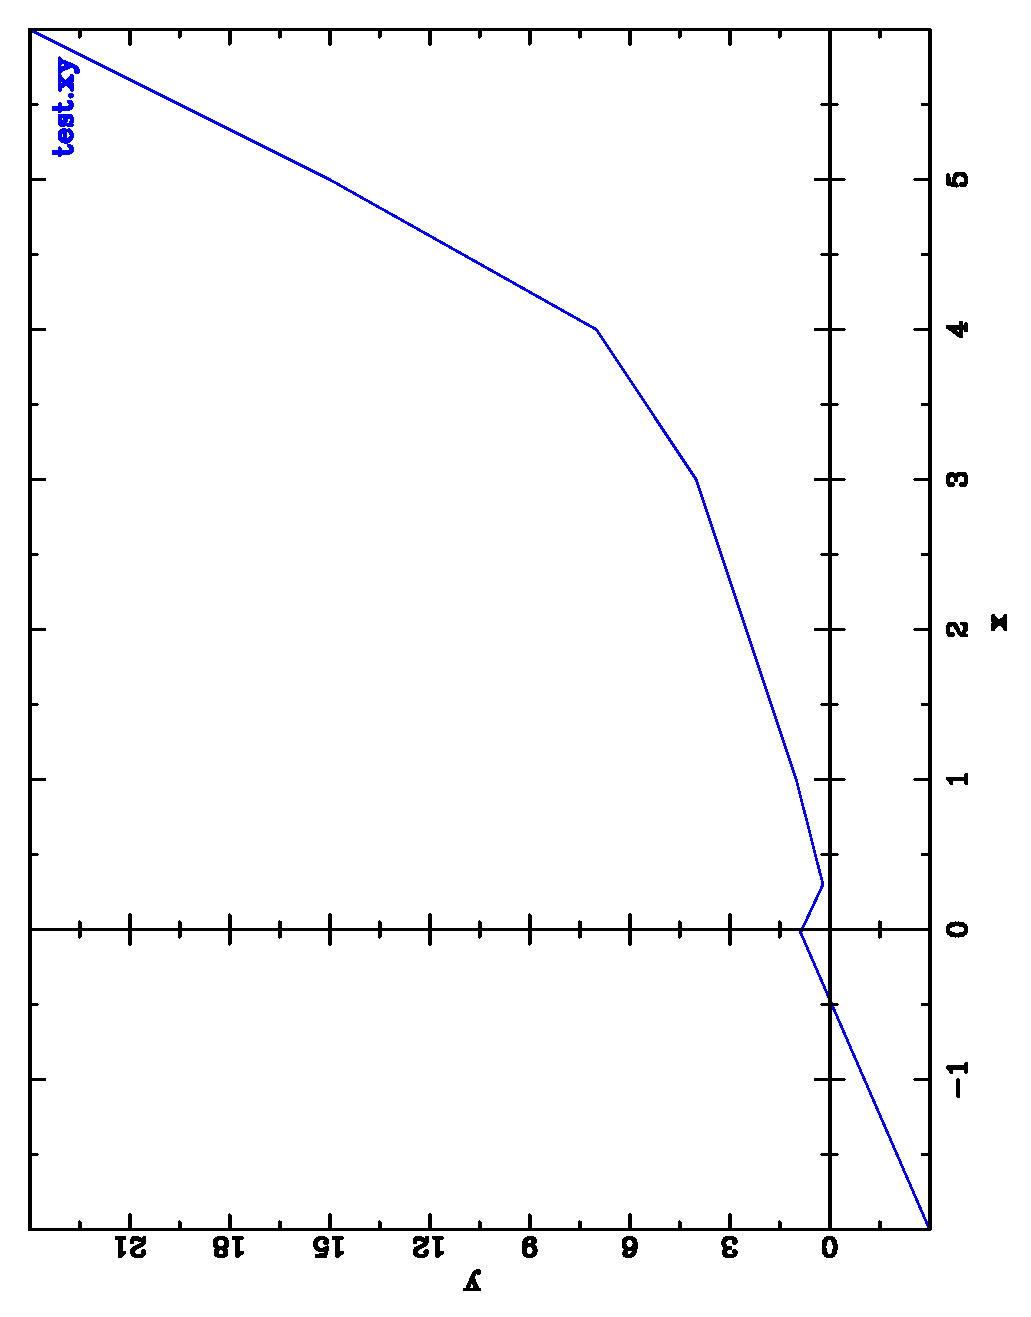
\includegraphics[width=3.0in, angle=270.0]{pl1.1.eps}
   \caption{The first {\it KUPLOT} plot}
   \label{pl1-fig1}
\end{figure}

The simplest data file is a text file with x- and y-coordinates
($x_{i},y_{i}$) for each point in a separate line, as in the example
data file {\it test.xy} listed below:
%
\begin{MacVerbatim}
    -2.00 -3.00
    -0.02  0.87
      :     :
\end{MacVerbatim}
%
In order to plot the file {\it test.xy}, we only need to enter the
following two commands at the {\it KUPLOT} input prompt:
%
\begin{MacVerbatim}
    load xy,test.xy
    plot
\end{MacVerbatim}
%
The {\tt load} command reads the specified data file, which is in
our case of the type 'xy'. The command {\tt plot} finally displays
the plot on the screen. The resulting plot for this example can be
seen in Figure \ref{pl1-fig1}. The following sections of this
chapter describe the supported file formats and how to change, print
and save the resulting plots.

%------------------------------------------------------------------------

\section{File formats \label{1d-read}}

{\it KUPLOT} reads data sets using the 'load' command.  The simplest
file format is a text file containing values for $x$ and $y$ on a
separate line for each data point as in the previous example.  To
read more than one data set just repeat the {\tt load} command.  The
maximum number of data sets that can be read and the maximum total
number of data points are defined in the file {\it kuplot.inc} and
might be adjusted before {\it KUPLOT} is compiled. The current
limits can be displayed using the command {\tt show config}. The
{\tt rese} command clears the currently loaded data sets and the
next file is read as data set one again. \par

The various file formats for 1D data supported by {\it KUPLOT} are
summarized in Table \ref{pl1-tab1}. The file format is specified as
first parameter for the {\tt load} command followed by the name of
the file to be read. Note that the 'xy' and 'yx' formats may contain
standard deviations $\sigma_{x}, \sigma_{y}$ for each data point
which may be used to plot error bars using the {\tt etyp} command in
{\it KUPLOT}. Optional parameters for the command {\tt load xy}
allow one to assign columns in the data file to $x, y$ and
$\sigma_{x}, \sigma_{y}$. The following command for example will
assign column 2 to $x$, column 4 to $y$ and column 9 to $\sigma_{x}$
and 12 to $\sigma_{y}$:
%
\begin{MacVerbatim}
    load xy,datafile.dat,2,4,9,12
\end{MacVerbatim}
\par

\begin{table}[!bt]
\centering
\begin{tabularx}{\textwidth}{|p{15mm}|X|}
  \hline
  {\bf Format} & {\bf Description} \\
  \hline\hline
  cr   & Special crystal structure format exported by {\it DISCUS}.
         Each line contains $x$,$y$,$z$, marker type, color and
         marker size for the atom at the given coordinates. Note,
         the first two columns are uses for plotting, the $z$ value
         is ignored (see {\it DISCUS} plot sublevel). \\
  ma   & Only the $x$ value of each data line is read, $y$ is set to
         zero. This allows the plotting of tick marks (e.g. at Bragg peak
         positions) at the x-axis. \\
  sc/st & This command allows one to read scans from a SPEC file.\\
  gs   & This command allows one to read GSAS files.\\
  xx   & Each line contains only one value that is taken as $y$
         value and the point number is stored as $x$ value. \\
  xy   & Each line of the data file contains $x$,$y$ and optionally
         standard deviations $\sigma_{x}$ and $\sigma_{y}$ from a
         multi-column text file. The default is $x,y,\sigma_x,\sigma_y$,
         but the columns can also me manually assigned (see example).\\

  \hline
  special & Various other file formats are available to read specific
            information from data files created by the diffractometer
            control software for the instruments MAN I and MAN II at
            the FRM I.  For details refer to the online help for the
            command {\tt load}.\\
  \hline
\end{tabularx}
\caption{\label{pl1-tab1}Supported file formats for 1D data}
\end{table}

After a data set is read, {\it KUPLOT} displays the number of points
read and the x- and y-limits. In our previous example, the screen
output after entering the {\tt load xy,test.xy} looks like that:
%
\begin{MacVerbatim}
    Reading 2 columns ...
    Data set no.:   1

      Filename : test.xy                            (     8 points )
      Range  x :   -2.000     to    6.000
      Range  y :   -3.000     to    24.00
\end{MacVerbatim}
%
Since our example file contains no $\sigma$ values, {\it KUPLOT} can
only read two columns. The file is associated with data set 1. This
data set number is subsequently used to alter the appearance of the
plot for a given data set (see section \ref{1d-change}).

\subsection*{Reading SPEC files}

As mentioned earlier, {\it KUPLOT} can read so called SPEC files.
Basically a SPEC file can contain several scans, each consisting of
multiple columns. One can use {\it KUPLOT} to get basic information
about the file contents: {\tt load st,spec.dat} will simple list all
scans in the file, but load no actual data. The command {\tt load
st,spec.dat,1} will list the columns available in scan number one.
Again no actual data are loaded. An example output is shown here:
%
\begin{MacVerbatim}
   kuplot > load st,npdf_02305.sqa
   Reading file npdf_02305.sqa ..
   List of scans in file npdf_02305.sqa :
     6536 pts --> #   1 Bank at   46.00 degrees
     6536 pts --> #   2 Bank at   90.00 degrees
     6536 pts --> #   3 Bank at  119.00 degrees
     6536 pts --> #   4 Bank at  148.00 degrees

   kuplot > load st,npdf_02305.sqa,2
   Reading file npdf_02305.sqa ..
   ---------------------------------------------
   Scan    2 in file npdf_02305.sqa :
   ---------------------------------------------
     Data field    1 : Q
     Data field    2 : S
     Data field    3 : sigmaS
     Data field    4 : F
     Data field    5 : sigmaF
\end{MacVerbatim}
%
If we now want to read $Q, F(Q)$ and $\sigma(F(Q))$ from bank or
scan number two, we simply need to specify the desired columns after
the scan number as show here:
%
\begin{MacVerbatim}
   kuplot > load st,npdf_02305.sqa,2,1,4,0,0,5
   Reading file npdf_02305.sqa ..
   --------------------------------------------
   Scan    2 in file npdf_02305.sqa :
   --------------------------------------------
     Axis x is       :               Q (#   1)
     Axis y is       :               F (#   4)
     Error column dy :          sigmaF (#   5)

   ...
\end{MacVerbatim}
%
The scan number is 2 and columns 1 and 4 are assigned to $x$ and
$y$. The next parameter specifies a column used to normalize the $y$
value, e.g. a measuring time. A value of zero tells {\it KUPLOT} to
ignore this parameter. The last two numbers are the columns for
$\sigma_x$ and $\sigma_y$ and again the zero for $\sigma_x$
indicates that no errors for $x$ should be read and are in fact not
present in our example file. The scan number can also be specified
as {\tt all} in which case all scans preset in the file are loaded
as separate datasets into {\it KUPLOT}.

\subsection*{Reading GSAS files}

GSAS is a structure refinement program and we refer to powder
diffraction data files in a format compatible with that program as
GSAS files. This format is particularly common for time-of-flight
neutron powder diffractometers. Similar to a SPEC file, it contains
data for several scans or more commonly called banks. Similar to
before, the command {\tt load gs,file.gsa} will list the banks
present in the file. Once a bank number or {\tt all} is added to the
command, the corresponding data are read as in this example reading
data from bank 1:
%
\begin{MacVerbatim}
    load gs,file.gsa,1
\end{MacVerbatim}
%
Additional optional parameters allow one to select the units for he
$x$-axis. Valid units are time-of-flight (t), d-spacing (d),
momentum transfer Q (q) and wavelength (l). In addition data can be
normalized by the incident neutron spectrum in case of spallation
neutron data. Most of these conversions require a so-called
instrument parameter file which is also needed to run GSAS itself.
Let us look at an example
%
\begin{MacVerbatim}
    load gs,file.gsa,all,d,iparm.dat,norm
\end{MacVerbatim}
%
Here we read all banks from the file {\it file.gsa} and convert the
$x$-axis to d-spacing. The instrument parameter file is {\it
iparm.dat} and the last parameter {\tt norm} causes the data to be
normalized by the incident spectrum. As a side note, the incident
spectrum is calculated from parameters given in the instrument
parameter file. Refer to the GSAS documentation for more details.


%------------------------------------------------------------------------

\begin{figure}[!b]
   \centering
   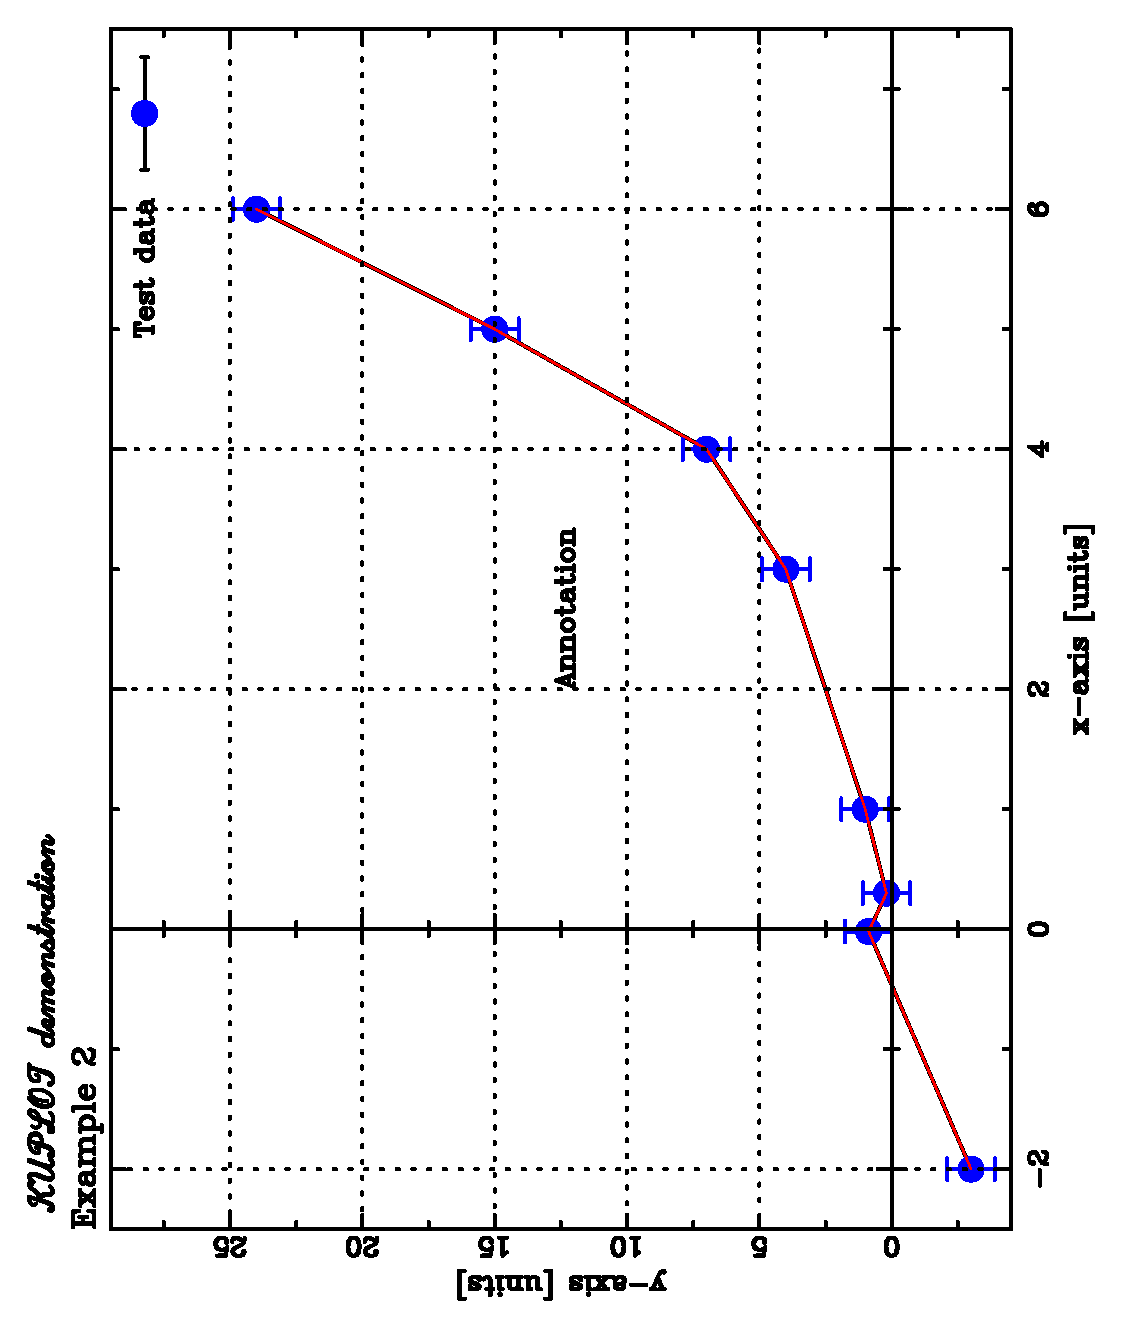
\includegraphics[width=3.0in, angle=270.0]{pl1.2.eps}
   \caption{Customized {\it KUPLOT} plot}
   \label{pl1-fig2}
\end{figure}

\section{Making a nicer plot \label{1d-change}}

In the example shown in Figure \ref{pl1-fig1} we have simply used
the defaults of {\it KUPLOT} and plotted the data set directly. The
program {\it KUPLOT} offers a variety of commands to alter the
appearance of the plot itself and the representation of each loaded
data set. We are using the same data set {\it test.xy} as in the
previous example (with added $\sigma$ values) and create the plot
shown in Figure \ref{pl1-fig2}. The macro file used to create this
plot is listed below. Note, that the line numbers are added for easy
reference within this manual and are not part of the actual macro
file.
%
\begin{MacVerbatim}
      1  load xy,test.xy
      2  #
      3  achx x-axis [units]
      4  achy y-axis [units]
      5  tit1 \fs KUPLOT demonstration
      6  tit2 Example 2
      7  #
      8  grid on
      9  fnam off
     10  #
     11  skal -2.5,7.5,-4.5,29.5
     12  mark 2,5
     13  #
     14  lcol 1,6
     15  lwid 1,0.5
     16  mtyp 1,3
     17  mcol 1,3
     18  msiz 1,0.4
     19  etyp 1,2
     20  #
     21  sleg 1,"Test data"
     22  sann 1,"Annotation",2,12
     23  plot
\end{MacVerbatim}
%
In line 1 of this macro we read the data set from file {\it test.xy}
as in the previous example.  The axes labels and the text for the
first and second title line are set in lines 3--6. The grid of
dashed lines at positions of the major tick marks is enabled in line
8 and the plotting of the filenames corresponding to the data sets
in the upper left corner of the plot is switched off (line 9). Next
we define the extend of the plot (line 11) to be from -2.5 to 7.5 in
the x-direction and from -4.5 to 29.5 in the y-direction. The tick
mark interval is set to 2.0 and 5.0 (line 12). All these settings
affected the complete plot, whereas the following commands act on
data set 1, which is given as the first parameter to all commands in
lines 14--19.  First the line color is set to black (line 14).  The
first six colors are coded as the 6 default pen colors on a HP
plotter, i.e.  red, green, blue, purple, yellow and black. Those
default colors can be redefined using the command {\tt color}.  In
the following lines, the line width, marker type, marker color and
marker size are defined (lines 16--18).  The different marker types
supported by {\it KUPLOT} are shown in Figure \ref{pl1-fig3}. In
addition to the markers shown, {\it KUPLOT} can access all markers
defined in the {\it PGPLOT} library. The marker number is simply 100
plus the {\it PGPLOT} marker code. Refer to the {\it PGPLOT}
documentation for a list of those markers. Error bars in y-direction
based on the $\sigma_{y}$ values read from the input file {\it
test.xy} are enabled in line 19. Marker types -1, -2 and -3 will
plot the $x$, $y$ or $x,y$ coordinated instead of a marker symbol.
The caption "Test data" is defined in line 21 and the annotation
"Annotation" at the coordinates (2.0,12.0) is specified by the {\tt
sann} command in line 22. Note, the value 1 in line 30 stands for
the first annotation and not for data set one. Finally the plot is
displayed on the screen (line 23).
%
\begin{figure}[!tb]
   \centering
   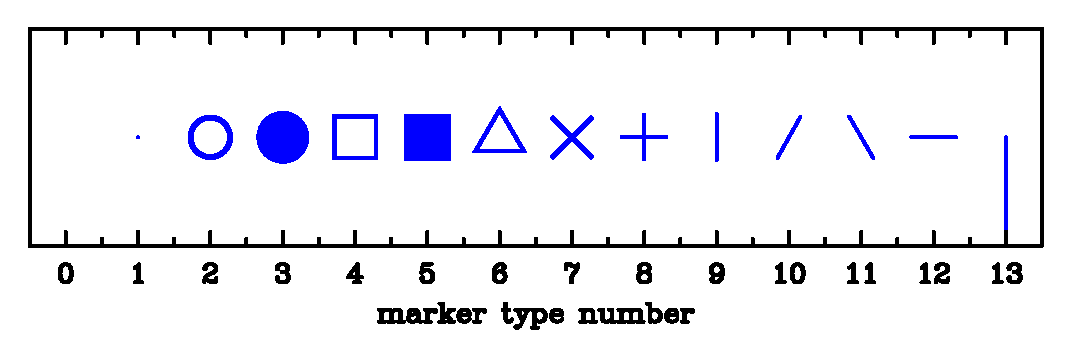
\includegraphics[scale=0.6]{pl1.3.eps}
   \caption{{\it KUPLOT} marker types}
   \label{pl1-fig3}
\end{figure}
%
\begin{figure}[!tb]
   \centering
   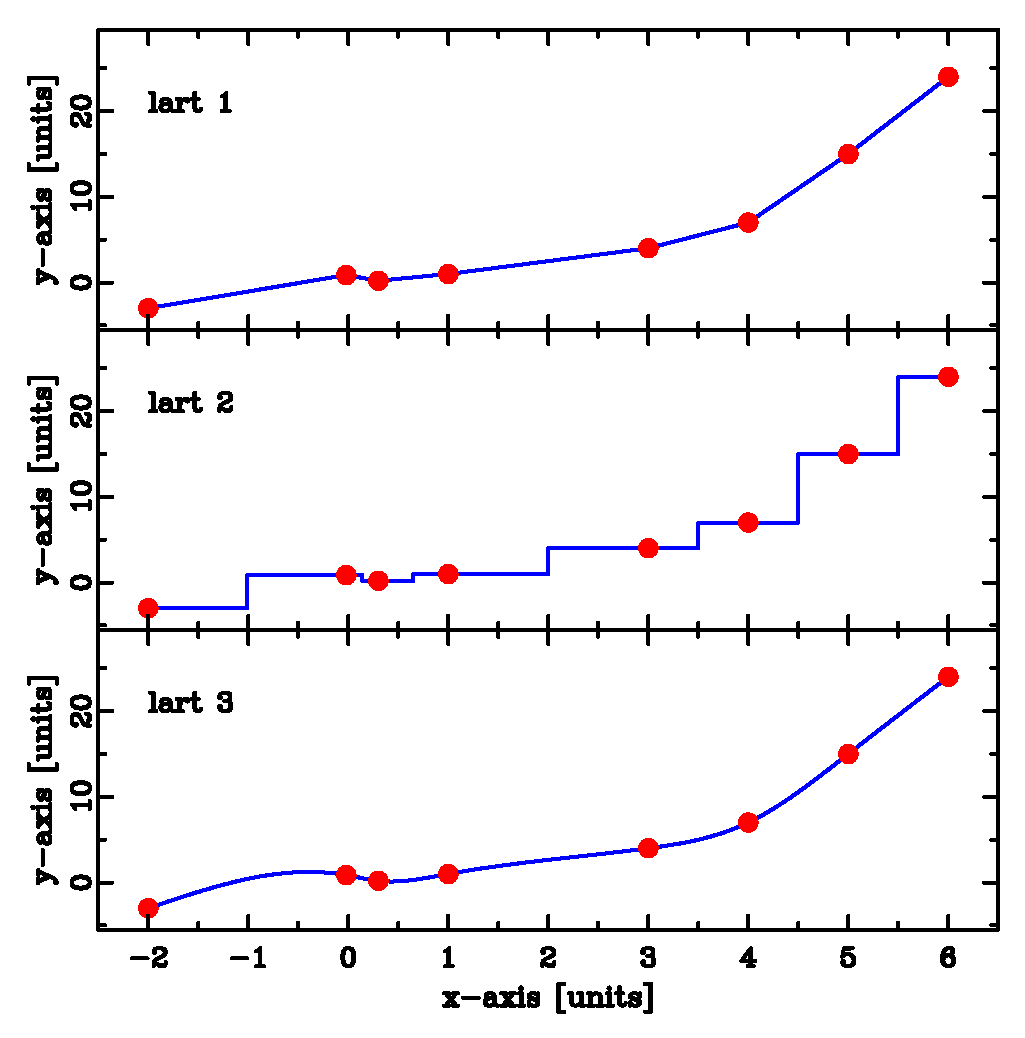
\includegraphics[scale=0.6]{pl1.4.eps}
   \caption{{\it KUPLOT} plotting styles}
   \label{pl1-fig4}
\end{figure}
%
In this example, the data points $(x_{i},y_{i})$ were simply
connected by a straight line.  {\it KUPLOT} offers two alternative
plotting styles: a histogram style and cubic spline interpolation.
The style is selected by the {\tt lart} command followed by the data
set number and the desired style. Style 1 is the default and
connects the data points by a straight line as in the previous
example ({\tt lart 1,1}).  This style is shown in Figure
\ref{pl1-fig4} in the bottom view graph.  The histogram style 2 is
shown in the middle view graph of the same Figure.  Here each data
point $(x_{i},y_{i})$ sits in the center of a histogram step. The
command to change the plotting style of data set 1 to histogram
would be {\tt lart 1,2}. The third mode ({\tt lart 1,3} for data set
1) is cubic spline interpolation. The interpolated spline goes
through all data points $(x_{i},y_{i})$ and has a continuous first
derivative. The spline interpolation of the data set {\it test.xy}
can be seen as top view graph in Figure \ref{pl1-fig4}. The default
number of interpolated points for a plot is 500. However, the value,
determined by the variable {\it MAXSP} might be altered in the file
{\it kuplot.inc} before {\it KUPLOT} is compiled.

%------------------------------------------------------------------------

\section{Fonts and special characters \label{1d-char}}

The program {\it KUPLOT} offers the user various ways to alter the
appearance of the text parts of the plot. All these functions are
accessed by the command {\tt font}. If no parameters are given, the
current settings will be displayed on the screen, as shown below:
%
\begin{table}[!bt]
\centering
\begin{tabularx}{\textwidth}{|c|X|}
  \hline
  {\bf Command} & {\bf Function} \\
  \hline\hline
   $\backslash$u  & start superscript, or end subscript \\
   $\backslash$d  & start sub-, or end superscript \\
   $\backslash$b  & backspace (draw next character on top of current one) \\
   $\backslash$fn & switch to normal font (1) \\
   $\backslash$fr & switch to roman font  (2) \\
   $\backslash$fi & switch to italic font (3) \\
   $\backslash$fs & switch to script font (4) \\
  \hline
   $\backslash\backslash$  & backslash  \\
   $\backslash$x  & multiplication sign $\times$ \\
   $\backslash$.  & centered dot $\cdot$ \\
   $\backslash$A  & \AA \\
  \hline
\end{tabularx}
\caption{\label{pl1-tab2}Text control characters}
\end{table}
%
\begin{MacVerbatim}
   Font settings for frame no.:   1
      Overall font scaling factor  :   2.50

      Font  where ?              size   fontname            font-id   color
      ---------------------------------------------------------------------
        1   Main title line       16.  Roman                    2       6
        2   Subtitle line         14.  Roman                    2       6
        3   Axis labels           12.  Roman                    2       6
        4   Numbers at axis       12.  Roman                    2       6
        5   Text in text frame    12.  Standard                 1       6
        6   Filename & caption    12.  Roman                    2       6
\end{MacVerbatim}
%
As can be seen from the output, there are six different types of
fonts, the main and second title line, the axis labels, the axis
numbering, text in a text frame (see section \ref{frame}) and
finally the font used for annotations and captions. Each of those
types is associated with a font size given in points, a font style
given as name (e.g. Roman) and number (e.g. 2) and finally a color
in our example pen number 6 or black. The four font styles
available in {\it KUPLOT} are shown in Figure \ref{pl1-fig5}. {\it
KUPLOT} allows the user to apply an overall scale factor to the
font size or change font sizes individually. As an example let us
change the color of the first title line to red. This would be
done using the command:
%
\begin{MacVerbatim}
    font col,1,1
\end{MacVerbatim}
%
The first parameter tells {\it KUPLOT} what we want to change,
here the color. Next we have the number of the font type, here 1
for the first title line. Finally we specify the desired color,
here pen 1 for red. One benefit of using the {\it PGPLOT} library
is that the user can access special characters and commands within
all text lines, e.g. titles, axis labels and text in text frames.
The supported control commands are listed in Table \ref{pl1-tab2}
and a list of Greek characters is given in Table \ref{pl1-tab3}.
For example to create an axis label \AA$^{-2}$ the text input
would read {\it $\backslash$A$\backslash$u-2$\backslash$d}. Note
that sub- and superscript always have to be given in pairs.
%
\begin{table}[!tbp]
\centering
\begin{tabular}{|c|cc|cc||c|cc|cc|}
  \hline
   alpha   & $\backslash$ga  & $\alpha$   & $\backslash$gA &   $A$        &
   beta    & $\backslash$gb  & $\beta $   & $\backslash$gB &   $B$        \\
   gamma   & $\backslash$gg  & $\gamma$   & $\backslash$gG &   $\Gamma$   &
   delta   & $\backslash$gd  & $\delta$   & $\backslash$gD &   $\Delta$   \\
   epsilon & $\backslash$ge  & $\epsilon$ & $\backslash$gE &   $E$        &
   zeta    & $\backslash$gz  & $\zeta $   & $\backslash$gZ &   $Z$        \\
   theta   & $\backslash$gh  & $\theta$   & $\backslash$gH &   $\Theta$   &
   iota    & $\backslash$gi  & $\iota $   & $\backslash$gI &   $I$        \\
   kappa   & $\backslash$gk  & $\kappa$   & $\backslash$gK &   $K$        &
   lambda  & $\backslash$gl  & $\lambda$  & $\backslash$gL &   $\Lambda$  \\
   mu      & $\backslash$gm  & $\mu   $   & $\backslash$gM &   $M$        &
   nu      & $\backslash$gn  & $\nu   $   & $\backslash$gN &   $N$        \\
   xi      & $\backslash$gc  & $\xi   $   & $\backslash$gC &   $\Xi   $   &
   omicron & $\backslash$go  & $o     $   & $\backslash$gO &   $O     $   \\
   pi      & $\backslash$gp  & $\pi   $   & $\backslash$gP &   $\Pi   $   &
   rho     & $\backslash$gr  & $\rho  $   & $\backslash$gR &   $P     $   \\
   sigma   & $\backslash$gs  & $\sigma$   & $\backslash$gS &   $\Sigma$   &
   tau     & $\backslash$gt  & $\tau  $   & $\backslash$gT &   $T     $   \\
   upsilon & $\backslash$gu  & $\upsilon$ & $\backslash$gU &   $\Upsilon$ &
   phi     & $\backslash$gf  & $\phi  $   & $\backslash$gF &   $\Phi  $   \\
   chi     & $\backslash$gx  & $\chi  $   & $\backslash$gX &   $X     $   &
   psi     & $\backslash$gq  & $\psi  $   & $\backslash$gQ &   $\Psi  $   \\
   omega   & $\backslash$gw  & $\omega$   & $\backslash$gO &   $\Omega$   &
           &                 &            &                &              \\
  \hline
\end{tabular}
\caption{\label{pl1-tab3}Access to Greek characters}
\end{table}
%
These examples can only give a brief introduction in the different
commands of {\it KUPLOT} allowing the user to alter the appearance
of the plot. For details on these commands and their parameters
refer to the online help, the command reference or the interactive
tutorial.
%
\begin{figure}[!tb]
   \centering
   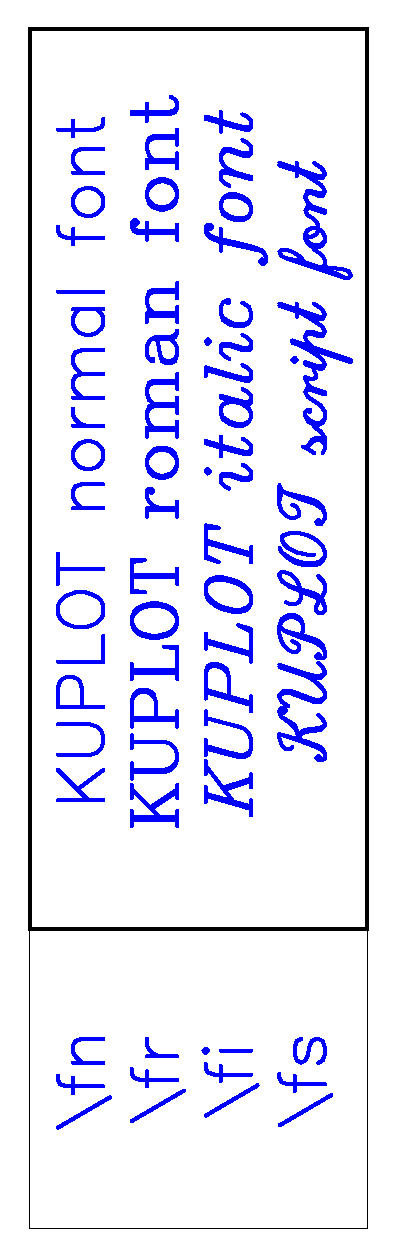
\includegraphics[scale=0.5, angle=270.0]{pl1.5.eps}
   \caption{{\it KUPLOT} fonts}
   \label{pl1-fig5}
\end{figure}

%------------------------------------------------------------------------

\section{Drawing bonds \label{1d-bond}}

The program {\it KUPLOT} allows the user to connect points in the
plot that are separated by a given distance. The distance is
specified relative to the current x-axis. To calculate the
distances, the aspect ratio and the angle between the axes is used.
These values can be defined by the user via the commands {\tt aver}
and {\tt angl} as we will discuss in somewhat more detail in section
\ref{2d-change}. Consequently you will get the desired connection
only for the correct aspect ratio and angle between the axes. This
feature can be used to include bonds when plotting a structure file
exported by {\it DISCUS}. An example for the compound PHTP
(Perhydrotriphenylen) is shown in Figure \ref{pl1-fig6}. The macro
file used to create this picture is listed below:
%
\begin{MacVerbatim}
      1  rese
      2  load cr,phtp.cr
      3  #
      4  skal 0.0,28.8,0.0,28.8
      5  mark 14.4,14.4
      6  #
      7  aver 1.0
      8  angl 120.0
      9  #
     10  msiz 1,0.35
     11  grid on
     12  fnam off
     13  #
     14  achx a-axis (\A)
     15  achy b-axis (\A)
     16  #
     17  bond 1,1.4,0.2,1,1,1.5
     18  #
     19  plot
\end{MacVerbatim}
%
First we reset the program and read the data (line 2). In line 4 the
plot area is defined followed by the setting for the tick mark
interval (line 5). In our case the lattice parameter is
$a=b=14.4$\AA. The command {\tt aver} defines the ratio between
units on the y- and x-axis. Since both are in \AA, the desired ratio
is one. The angle between the axes is set to 120$^{\circ}$ (line 8).
Next we set the marker size (line 10), turn the plotting of the grid
on (line 11) and disable the plotting of the filenames (line 12).
The axes labels are set in lines 14 and 15. So far nothing new, now
comes the command {\tt bond} that defines the bonds between carbon
atoms we like to plot. The first parameter 1 is the number of the
bond definition. {\it KUPLOT} allows one to define multiple
distances. The second and third parameter set the distance to
$1.4$\AA\ $\pm 20$\%. The last optional parameters in line 17 set
the bond color to red (pen 1), select a solid line (type 1) and set
the line width to $1.5$. All that remains is to plot the result
(line 19). One should be aware that {\it KUPLOT} calculates the
distances between {\it all} data points and compares the to the
selected distance interval which can be rather slow for large data
file. To disable a bond definition simply reenter the command with
distance zero, e.g. {\tt bond 1,0.0}.
%
\begin{figure}[!tb]
   \centering
   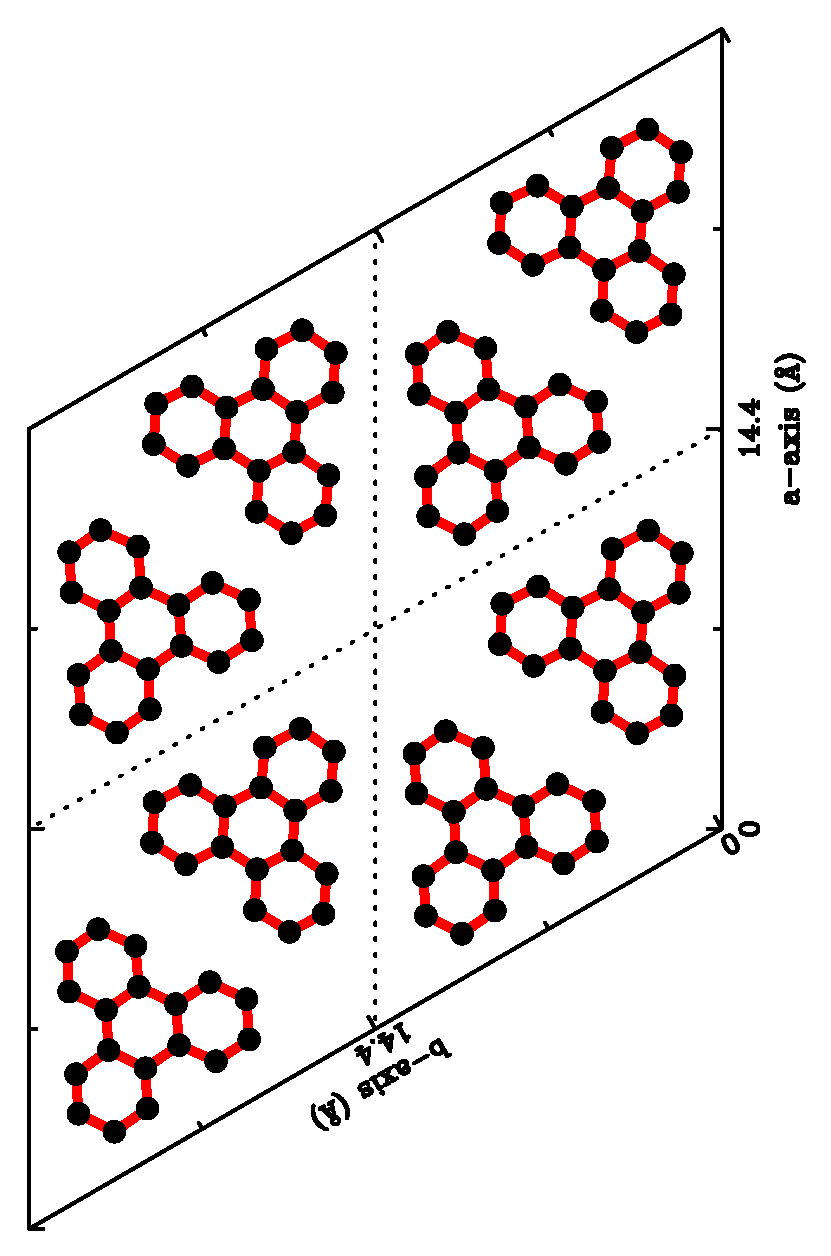
\includegraphics[scale=0.5, angle=270.0]{pl1.6.eps}
   \caption{Example for plotting bonds}
   \label{pl1-fig6}
\end{figure}

%------------------------------------------------------------------------

\section{Filling of areas\label{1d-fill}}

Sometimes to enhance the visibility of plot, it is desired to fill
the area under a data set. A plot taken from our recent book {\it
Diffuse scattering and defect structure simulations - A cook book
using the program DISCUS} published by Oxford University Press is
shown in Figure \ref{pl1-fig6b}.
%
\begin{figure}[!tb]
   \centering
   \includegraphics[scale=0.5, angle=0.0]{pl1.6b.eps}
   \caption{Example for filling areas}
   \label{pl1-fig6b}
\end{figure}

The part setting the colors and filling options of the macro file
used to create the plot is shown here.

\begin{MacVerbatim}
   color 1,0.8,0.8,0.8
   color 2,0.6,0.6,0.6
   color 3,0.4,0.4,0.4
   #
   fill 1,3,5
   fill 2,2,5
   fill 3,1,5
\end{MacVerbatim}
%
The command {\tt color} sets the color for the different 'pens' of
{\it KUPLOT}. In this case colors one through three are assigned
three different shades of grey. The color is specified as red,
green, blue raging from 0 to 1. The command {\tt fill ik,c,t} then
selects filling for data set {\tt ik} using color or pen {\tt c} and
setting the fill style to {\tt f}. In our case style five
corresponds to a solid fill with a black border. Type {\tt help
fill} for a list of all fill styles.

%------------------------------------------------------------------------

\section{Saving data sets \label{1d-save}}

The program {\it KUPLOT} allows the user to save loaded data sets to
a file.  This might be necessary after a data set was altered or in
cases where only part of the data shall be saved.  To save a data
set, use the command {\tt ksav} followed by the number of the data
set to be saved.  After entering the {\tt ksav} sublevel, you need
to specify the output filename and the file format for the output
file. In this section we will only discuss the saving of 1D data
sets and the only available file format is {\tt xy} (see previous
example).  The following commands will save the loaded data set 1
(e.g.  {\it test.xy} from the example above):
%
\begin{MacVerbatim}
     1  ksav 1
     2    outfile export.xy
     3    form xy,0.0,5.0
     4    show
     5  run
\end{MacVerbatim}
%
In line 1 we enter the {\tt ksav} sublevel.  The parameter specifies
the data set we want to save, here data set 1.  Next the output
filename is set to {\it export.xy} (line 2).  The file format is set
to {\tt xy} and the optional further parameters give x-limits (line
3), i.e.  only data points with x-values between 0.0 and 5.0 will be
saved.  Note, that the default range are defined by the current plot
window limits.  Thus if the plot window set by the command {\tt
skal} is smaller than the extend of the actual data set, only point
that are visible in the current plot are saved if no limits are
given with the {\tt form} command.  The command {\tt show} (line 4)
lists the current limits and finally the data are written to the
specified file via the {\tt run} command (line 5).  The command {\tt
run} also exits the {\tt ksav} sublevel.  To exit without actually
writing a file use the {\tt exit} command.  \par

The {\tt ksav} command has many additional options to save 2D data
such as format conversion and the export of cross sections. These
functions are discussed in chapter \ref{2d-save}.

%------------------------------------------------------------------------

\section{Printing and exporting the plot \label{1d-print}}

Viewing the plot on the screen is one thing, but we certainly need
to print plot at some stage or save is for e.g. import in a text
processing program. {\it KUPLOT} supports two different output
formats that can be saved or used for printing. The defaults are
POSTSCRIPT and GIF associated with the parameters {\tt ps} and {\tt
pic} respectively. However, they can be set to any device supported
by {\it PGPLOT} by altering the variables {\it dev\_name} in the
file {\it blk\_appl.f} of the {\it KUPLOT} distribution. The
variable {\it dev\_prn} in the same file sets the default print
command. To print the current plot to the default printer, use {\tt
prin ps}. To reach other printers, the corresponding print command
can be specified as a second parameter to the {\tt prin} command as
in the example below:
%
\begin{MacVerbatim}
     prin ps,"lp -d myprinter -h "
\end{MacVerbatim}
%
Here the printer {\tt myprinter} is used. Check local documentation
or ask your system administrator how to access the desired printer.
In order to save the graphics file rather than printing it, use the
{\tt save} command with the first parameter being {\tt ps} or {\tt
pic} for POSTSCRIPT or GIF output respectively.  The second
parameter is the name of the output file, e.g. {\tt save
ps,plot.ps}.

%------------------------------------------------------------------------

%------------------------------------------------------------------------
% Chapter:  2D data plots
%------------------------------------------------------------------------

\chapter{Plotting 2D data \label {2d}}

In the previous chapter we have learned about using {\it KUPLOT}
to plot 1D data sets. Now we will extend the usage of {\it KUPLOT}
to 2D data sets, i.e. xyz-data. The coordinates $x$ and $y$ are
within the drawing plane and the $z$ values are represented by
contour lines at given $z_{c}$ values, by the bitmap color or
both. Changing the general appearance of the plot such as defining
title lines, labels or tick mark intervals was described in
section \ref{1d-change} of this manual and works exactly the same
way when plotting 2D data sets.

%------------------------------------------------------------------------

\section{File formats \label{2d-read}}

As described in section \ref{1d-read} for 1D data sets, 2D data sets
are read using the command {\tt load}. Multiple data sets might be
read by repeating the command {\tt load} and 1D and 2D data sets
might be imported in any combination. The command {\tt rese} clears
the currently loaded data sets and the next file is read as set
number one again.
\par

A summary of the supported 2D file formats is given in Table
\ref{pl2-tab1}. All file formats are "normal" text files that can be
viewed and edited with every text editor. Since these files are
normally larger in size compared to a binary version, archived files
might be compressed with standard UNIX tools like {\it compress} or
{\it gzip}. The standard file format for 2D data is the so-called
NIPL format which was developed at the Insitut f\"ur Mineralogie und
Kristallographie in M\"unchen. The NIPL format ({\tt ni}) is defined
as follows:

\footnotesize
\begin{MacVerbatim}
    1      nx ny
    2      xmin xmax ymin ymax
    3ff    z z z z ...
\end{MacVerbatim}
\normalsize

The first line contains the number of data points in x- and in y-direction.
The next line gives the x- and y-limits of the plot area.  All following
lines contain the z-values row by row starting in the lower left corner.
The z-values are real numbers and not restricted in any way.  However, the
value -9999.0 is reserved for excluded regions (see below).

\begin{table}[htb]
\centering
\begin{tabularx}{\textwidth}{|p{15mm}|p{30mm}|X|}
  \hline
  {\bf Format} & {\bf add. Parameters} & {\bf Description} \\
  \hline\hline
  de  &  $\Delta x,\Delta y$ & Reads xy-file and creates a 2D data
                    set with the number of points that are inside a
                    specified grid box $\Delta x,\Delta y$ as z-values.\\
  ni  &  [exclude] & Reads NIPL file format (see text). The optional
                     parameter is a file containing excluded regions. \\
  pg  &            & Reads PGM file format (see text). \\
  zz  &  $\Delta x,\Delta y$ & Reads xyz-file and bins the data to the
                     given grid size $\Delta x,\Delta y$ \\
  \hline
\end{tabularx}
\caption{\label{pl2-tab1}Supported file formats for 2D data}
\end{table}

The optional third parameter listed in Table \ref{pl2-tab1} is the
name of a file containing excluded regions, i.e.  areas of the data
file that should be excluded from the plot.  An example is shown in
Figure \ref{pl2-fig1}.  The plot on the bottom was created by
reading the NIPL file {\it test.nipl} using the command {\tt load
ni, test.nipl} and thus reading all data.  The data shown here are
actually neutron diffuse scattering from calcium stabilised zirconia
collected by R.B.  Neder at the neutron source in Garching, Germany.
Sometimes one wants to exclude certain regions within the data from
the actual plot, in our example the strong Bragg peaks.  This can be
done by creating a file with coordinates of rectangles within the
plotting area that should be excluded.  Such a file can be created
using a text editor.  In our example, the excluded region file {\it
test.excl} looks like this:

\begin{MacVerbatim}
 10
 0.87  1.13  0.81  1.17
 2.85  3.15  0.81  1.26
 1.85  2.34  3.70  4.28
 2.82  3.18  2.79  3.28
 0.87  1.18  2.81  3.23
 0.00  0.24  3.68  4.28
 0.00  0.12  1.73  2.24
 0.00  0.58  0.00  0.79
 1.78  2.22  0.00  0.35
 1.90  2.17  1.81  2.13
\end{MacVerbatim}

The first line contains the number of rectangle coordinates in the
file followed by {\it xmin, xmax, ymin, ymax} for each excluded
region. Rereading the file {\it test.nipl} using the command {\tt
load ni, test.nipl, test.excl} results in the right view graph of
Figure \ref{pl2-fig1}.  Note that {\it KUPLOT} will replace all
z-values within an excluded region by -9999.0 and those values will
be ignored by most {\it KUPLOT} functions.  If a file read with
excluded regions is saved later on, the data within those excluded
regions are lost.

\begin{figure}[!tbh]
   \centering
   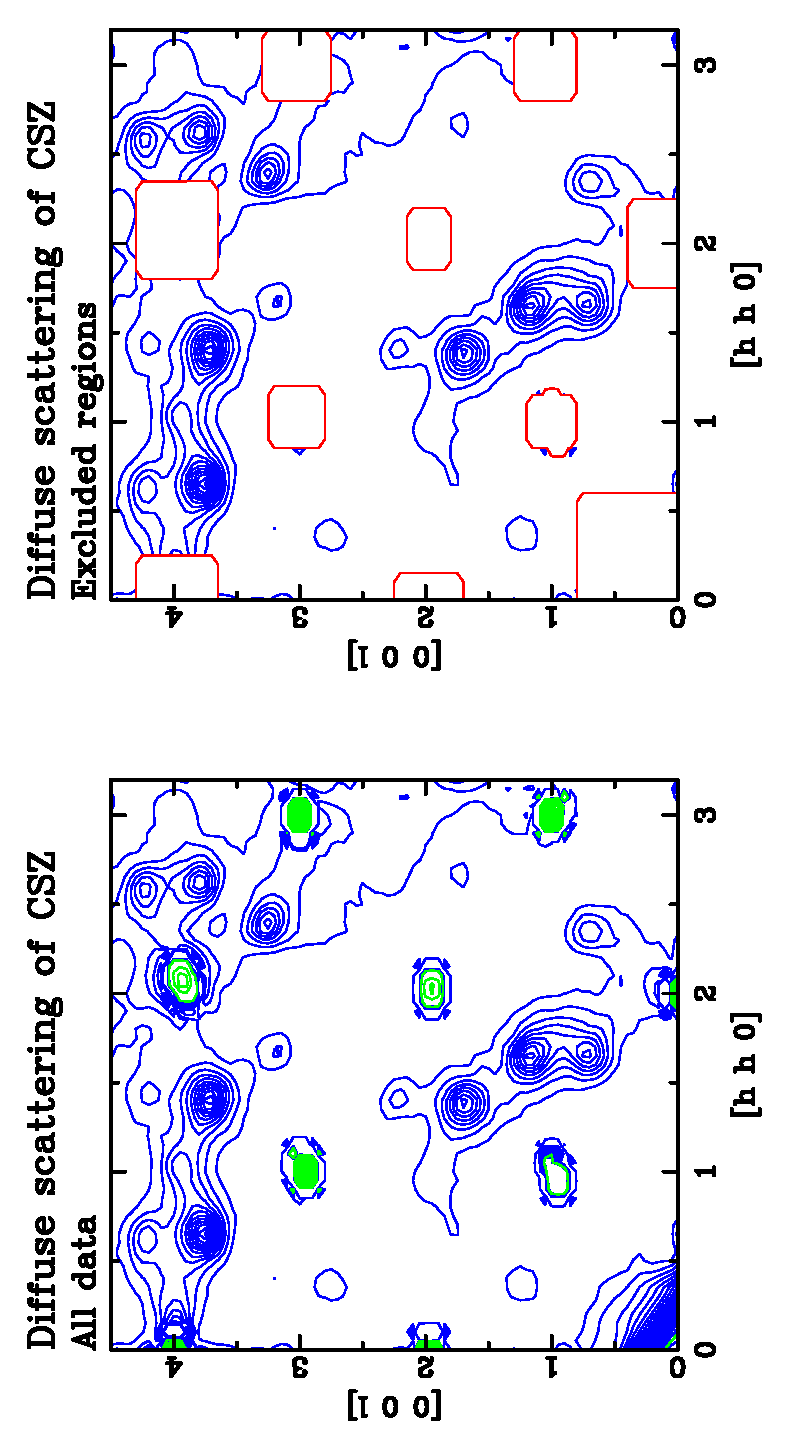
\includegraphics[scale=0.6, angle=270.0]{pl2.1.eps}
   \caption{Usage of excluded regions for 2D files}
   \label{pl2-fig1}
\end{figure}

The second more general 2D file format is the PGM (portable graymap)
format which is defined as part of the  PNM format Jef Poskanzer.
Various programs are capable of reading PNM files and the {\it
pnmplus-package} is a freely available collection of tools and
conversion programs from PNM to virtually any other graphics format.
{\it KUPLOT} only supports ASCII PGM files which are defined as
follows:

\begin{MacVerbatim}
    1      P2
    2      nx ny
    3      255
    4ff    z z z z z
\end{MacVerbatim}

The code {\it P2} in the first line identifies the file as ASCII PGM
format. The dimensions $nx$ and $ny$ of the data set are given in
the next line. The PGM format is an integer bitmap and the number in
line 3 gives the maximum depth (here 255 or 8 bit). Although the PGM
format is generally not restricted to 8 bit resolution, it was found
that many programs are not capable of reading PNM files with a
larger resolution. Comments can be included in the file starting
with a \# as first character. The actual data are integer values
written row by row starting (in contrast to NIPL files) from the top
left corner. Besides being limited to integer values ranging from $0
\rightarrow 255$, the PGM file format does not contain any
information about the $x$ and $y$ limits and {\it KUPLOT} sets x-
and y-values to the pixel number. However, the x- and y-values might
be manipulated (see chapter \ref{mat}) and the file can be saved in
NIPL format (see section \ref{2d-save}), thus allowing the
conversion of PGM files to NIPL files and {\it vice versa}.\par

The PGM and NIPL files are restricted to data points being on a
equidistant rectangular grid. The file format 'zz' can be used to
read any data file containing the data points $(x_{i}, y_{i},
z_{i})$ on a separate line. This is practically the extension of the
'xy' file format. However, {\it KUPLOT} can internally only work
with z-values lying on a rectangular equidistant grid. Thus the read
data points are binned to a grid size defined by $\Delta x$ and
$\Delta y$ given as additional parameters to the {\it load} command.
Each resulting grid point contains the average of all data points
within the file that fall within the area of the specific grid
point. If the specified grid size is too small, the resulting plot
will contain empty grid points. The following command reads the XYZ
file {\it test.xyz} and bins it to a grid size of $\Delta x = \Delta
y = 0.05$:

\begin{MacVerbatim}
    load zz,test.xyz,0.05,0.05
\end{MacVerbatim}

This file format can also be used to rebin data sets to a broader grid
by saving the NIPL (or PGM) file as XYZ file and rereading the file
with the new desired grid size. \par

The file format {\tt de} (for density) works similar to the
previously discussed {\tt zz} format but rather than averaging the
z-values in each grid point, the resulting z-value is the number of
points $(x_{i}, y_{i})$ falling within the corresponding grid volume
which is defined as before by the additional parameters $\Delta x$
and $\Delta y$. The program reads the first two real numbers in each
line as x- and y-value. For example {\it DISCUS} can export the atom
positions of all atoms without the translational part, i.e. all
atoms are in one unit cell. The resulting file can be read using the
{\tt cr} format resulting in a marker for each atom. Alternatively
the same file (since the first two numbers are $x$ and $y$) can be
read using the 'de' format which will result in a density plot which
can be displayed either using contour lines or a bitmap.

%------------------------------------------------------------------------

\section{Customizing the plot \label{2d-change}}

The command {\tt hart} selects the usage of contour lines, bitmaps
or both and is discussed in the next section. Here we want to
concentrate on commands used to change contour lines. The base
level, the interval and the number of contour line levels are
defined using the command {\tt hlin}:

\footnotesize
\begin{MacVerbatim}
    hlin 1,100,50,10
    hlin 2,10,10,9,%
\end{MacVerbatim}
\normalsize

{\it KUPLOT} supports multiple sets of contour lines, e.g.  one set
at low levels to display diffuse scattering and one set at higher
levels with a different spacing for the stronger Bragg peaks.  Each
set can be plotted in a different color.  The two example commands
above illustrate the {\tt hlin} command.  The first command sets the
values for contour line set 1.  The contours start at a value of 100
and increase in steps of 50.  A total of 10 contour levels is drawn,
e.g.  the highest level corresponds to 600. The second {\tt hlin}
commands sets values for the second contour line set, but the
additional parameter '\%' indicates, that the numbers are taken as
percentage of $\Delta z = zmax - zmin$ of all loaded data sets
rather than absolute z-values.  In our example the base level is
10\% of $\Delta z$, the contour lines are stepped in 10\% intervals
and 9 levels are plotted. Thus the highest level corresponds to
100\%.  The command {\tt hpak} determines how many contour line sets
are actually plotted.  The default is the usage of all sets defined
by the {\tt hlin} command.  Color and line type for the individual
contour line sets can be changed using the commands {\tt hcol} and
{\tt htyp}.

\begin{figure}[!tbhp]
   \centering
   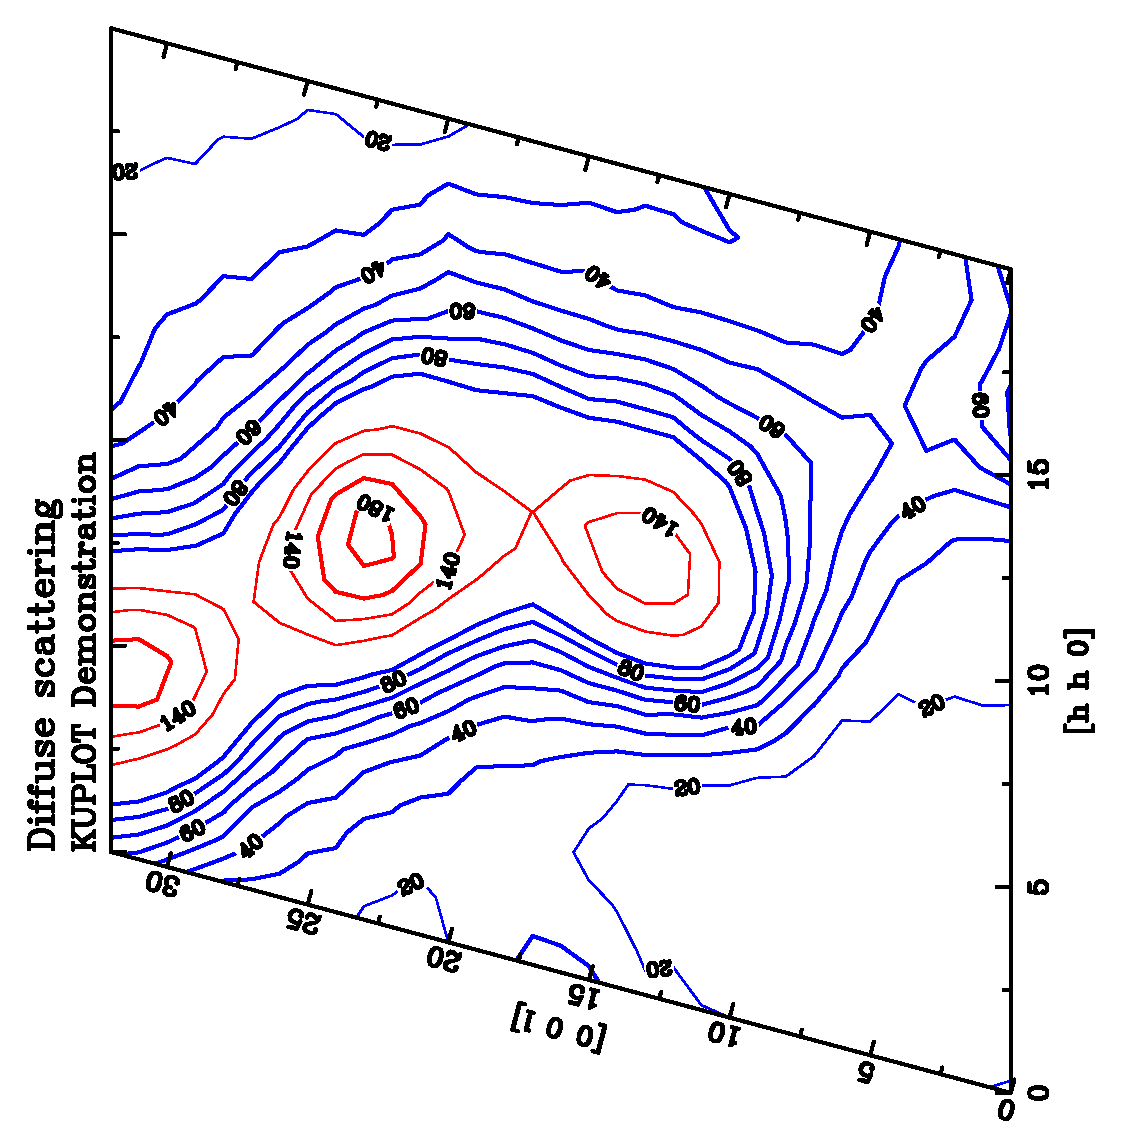
\includegraphics[scale=0.5, angle=270.0]{pl2.2.eps}
   \caption{Customizing contour plots}
   \label{pl2-fig2}
\end{figure}

Sometimes a specific aspect ratio of the x- and y-axis or a specific
angle between the two axis is required to obtain a non distorted
picture of the data.  {\it KUPLOT} allows the user to specify an
aspect ration using the {\tt aver} command.  As default {\it KUPLOT}
determines the aspect ratio is such a way, that the resulting plot
is as large as possible.  This default can be restored by entering
the command {\tt aver} without further parameters. Alternatively,
the desired ratio can be given as parameter to the {\tt aver}
command. In Figure \ref{pl2-fig2} we show an example of a contour
plot illustrating some of the features discussed above. The commands
used to create the contour lines shown are listed below:

\begin{MacVerbatim}
      1  aver 0.707
      2  angl 75.0
      3  #
      4  hlin 1, 10,10, 9
      5  hlin 2,120,20,10
      6  hcol 1,1,3
      7  hcol 1,2,1
      8  hlab 1,2
\end{MacVerbatim}

In line 1 we set the aspect ratio of the x- and y-axis to
$1/\sqrt{2} \approx 0.707$ and the angle between the axes to a value
of 75$^{\circ}$ (line 2). In lines 4--5 we define two contour line
packages, the first one giving contour lines at values of $z_{c} =
10, 20, ..., 100$ the second one at values $z_{c} = 120, 140, ...,
320$. In line 6 the color for the first contour package for data set
one is set to pen 3 (blue). Next the color for the second package
for the same data set is set to pen 1 (red). Finally the labeling of
contour lines for data set one is enabled. The second parameter in
line 8 specifies that every second contour line starting from the
base line is labeled. As always, check the online help for more
detailed information on the commands used.

%------------------------------------------------------------------------

\section{Using bitmaps \label{2d-bitmap}}

The command controlling the appearance of a 2D plot is {\tt hart}.
Its first parameter determines the data set, the second parameter
the type of plot. To use only contour lines set the second parameter
to 1, for bitmap display use 2 and to have both a bitmap and contour
lines set the second parameter of the {\tt hart} command to 3. In
Figure \ref{pl2-fig3} we can see the same plot using just a bitmap
on the bottom and using additional contour lines on the top. The
wedge showing the $z$ range of the bitmap colors is activated by
setting a label for the z-axis using the command {\tt achz}. \par

\begin{figure}[!tbhp]
   \centering
   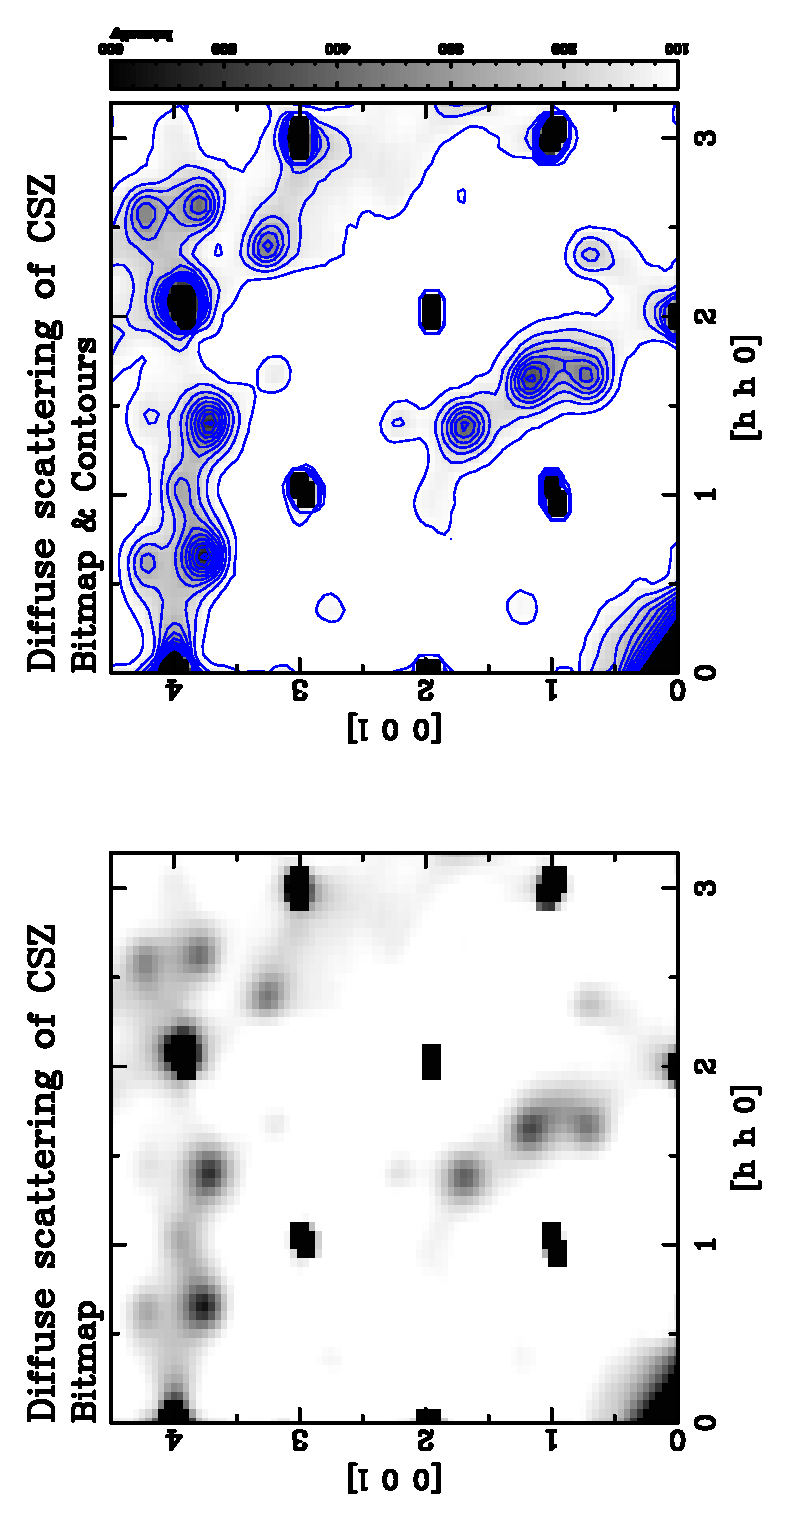
\includegraphics[scale=0.6, angle=270.0]{pl2.3.eps}
   \caption{Example for bitmap plots}
   \label{pl2-fig3}
\end{figure}

The bitmaps used by {\it KUPLOT} have 240 color entries, the
remaining 16 colors are reserved for other functions. The z-range to
be converted to those 240 colors is determined by the minimal and
maximal contour level for the first set defined by the command {\tt
hlin}. Subsequently the bitmap color range and the contour levels
are the same for the first set of contour levels. In some cases one
might want to create a plot where the bitmap and the contour lines
have different ranges. This can be done like in the following
example:

\begin{MacVerbatim}
    hlin 1,0,50,1,%
    hlin 2,0,5,20,%
    htyp 1,0
    htyp 2,1
\end{MacVerbatim}

The levels set by the first {\tt hlin} command determine the z-range
used to create the bitmap, i.e. 0\% to 50\% of the z-range. We do
this in a single step since only the maxima are used to determine
the bitmap. The second {\tt hlin} command sets the contour lines we
actually want to plot on top of the bitmap. In order to suppress the
first set of contour lines we set the line type for set 1 to 0, i.e.
no line using the first {\tt htyp} command. The line type for the
second contour set is set to 1, i.e. solid line, as done in the last
line of the example above. \par

{\it KUPLOT} has three default color maps used to display bitmaps.
The map is selected by the command {\tt cmap}. For a description of
the different color maps refer to the online help. The selected map
for the examples displayed in Figure \ref{pl2-fig3} is {\tt gray}.
The command {\tt cmap} is also used to save or read a color map from
a file. Additionally the current color map can be altered using the
variable {\it cmap}. For details about the usage of variables see
section \ref{var} of this users guide.

%------------------------------------------------------------------------

\section{Saving data \label{2d-save}}

\begin{figure}[!t]
   \centering
   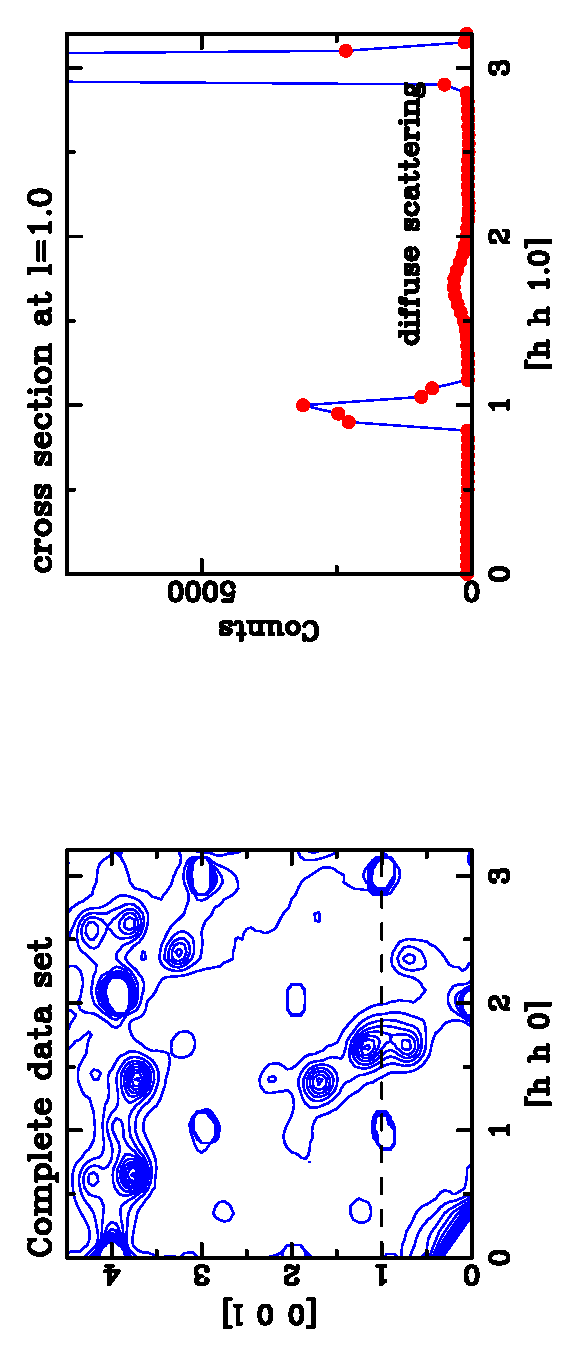
\includegraphics[scale=0.65, angle=270.0]{pl2.4.eps}
   \caption{Extracting data from 2D data sets}
   \label{pl2-fig4}
\end{figure}

In contrast to 1D data where we could mainly save a given data set
in the {\tt xy} format, there are several options to extract and
save data from a 2D data set. As described in section \ref{1d-save},
the first step is to enter the save sub level using the command {\tt
ksav} followed by the number of the data set to be saved. As before
the output filename is set by the command {\tt outfile} and the
saving process is started via {\tt run}. However, there are now many
more possible settings for the {\tt form} command.

\begin{table}[!b]
\centering
\begin{tabularx}{\textwidth}{|p{15mm}|p{45mm}|X|}
  \hline
  {\bf Format} & {\bf Parameters} & {\bf Description} \\
  \hline\hline
    ni & [x1,x2,y1,y2] & Nipl file, given area \\
    pg & [x1,x2,y1,y2] & PGM file (ASCII), given area \\
    gn & [x1,x2,y1,y2] & XYZ file (gnuplot), given area \\
  \hline
    sx & y-value       & Cross section $\|$ x at y-value \\
    sy & x-value       & Cross section $\|$ y at x-value \\
    mx & i             & Cross section $\|$ x through maximum \#i \\
    my & i             & Cross section $\|$ y through maximum \#i \\
    sk & ik            & Cross section along xy of data set ik \\
    sl & x1,y1,x2,y2,n & Cross section from x1,y1 to x2,y2 with n points \\
  \hline
\end{tabularx}
\caption{\label{pl2-tab2}Save options for 2D data sets}
\end{table}

The first three of those formats listed in Table \ref{pl2-tab2} save
the data set or a subsection as 2D data set either in NIPL, PGM or
XYZ format. As before the area that is saved is determined by the
current size of the plot window determined by the command {\tt
skal}. Alternatively the x-limits $x1$ and $x2$ and y-limits $y1$
and $y2$ can be specified as additional parameters to the 'form'
command. Note that when using PGM as output format, the z-values are
converted to integer and should range from $0 \rightarrow 255$. The
command 'thresh' allows to control how the z-values are converted to
this range. The other formats in Table \ref{pl2-tab2} are used to
extract a cross section from the 2D data set. The created output
file is a normal {\tt xy} file. The parameters {\tt sx} and {\tt sy}
extract a cross section parallel to the x- or y-axis at the given y-
or x-value (see example below). Rather than specifying these y- or
x-values, the corresponding coordinates of maximum $i$ determined by
the command {\tt smax} (see section \ref{mat}) can be used ({\tt mx}
or {\tt my}). The command above will extract the z-values at the
corresponding grid points. The last two options can extract data
from any value of $x$ and $y$ by interpolation. The format {\tt sk}
will use the coordinates $x$ and $y$ from data set (1D) number {\tt
ik} to determine the z-values to be extracted whereas {\tt sl} will
extract $n$ points along a straight line defined by the points
$(x1,y1)$ and $(x2,y2)$. \par

A simple example how to extract a cross section is show in Figure
\ref{pl2-fig4}. The original data set is shown on the left. The
cross section parallel x (or [hh0]) at y (or l) equals 1.0 is
marked by a dashed line. The resulting 1D plot of the cross
section is shown on the right panel of the figure. The
corresponding commands to create the data file shown at the top is
listed below:

\begin{MacVerbatim}
     1  ksav 1
     2  outfile test.cut
     3  form sx,1.0
     4  run
\end{MacVerbatim}

In line 1 we enter the save sub level. In our example the data set to
be used is data set number one. The output filename is set to {\it
test.cut} (line 2) and the format is set to {\tt sx}, i.e. cross
section parallel to $x$ at $y=1.0$ (line 3). Finally the data file
is written after the command {\tt run} is entered (line 4).


%------------------------------------------------------------------------

%------------------------------------------------------------------------
% Chapter:  Frames
%------------------------------------------------------------------------

\chapter{Using frames \label {frame}}

In this chapter we will introduce the usage of frames that enable
{\it KUPLOT} to display more than one view graph in a single plot. A
detailed description of all frame related commands is available as
part of the online help which can be accessed by entering {\tt help
frames} at the input prompt.

%------------------------------------------------------------------------

\section{Introduction \label{frame-int}}

Frames enable {\it KUPLOT} to display multiple view graphs within a
single plot. The layout is defined by the user. A simple example with
two graphs being plotted on a single page is shown in Figure
\ref{fra-fig1}. Let us have a look at the macro file that was used to
create the figure and learn step by step how to use this
feature of {\it KUPLOT}. Note that the line numbers shown in the
listing below are used for easy reference in this manual and are not
part of the actual macro file.

\begin{figure}[!b]
   \centering
   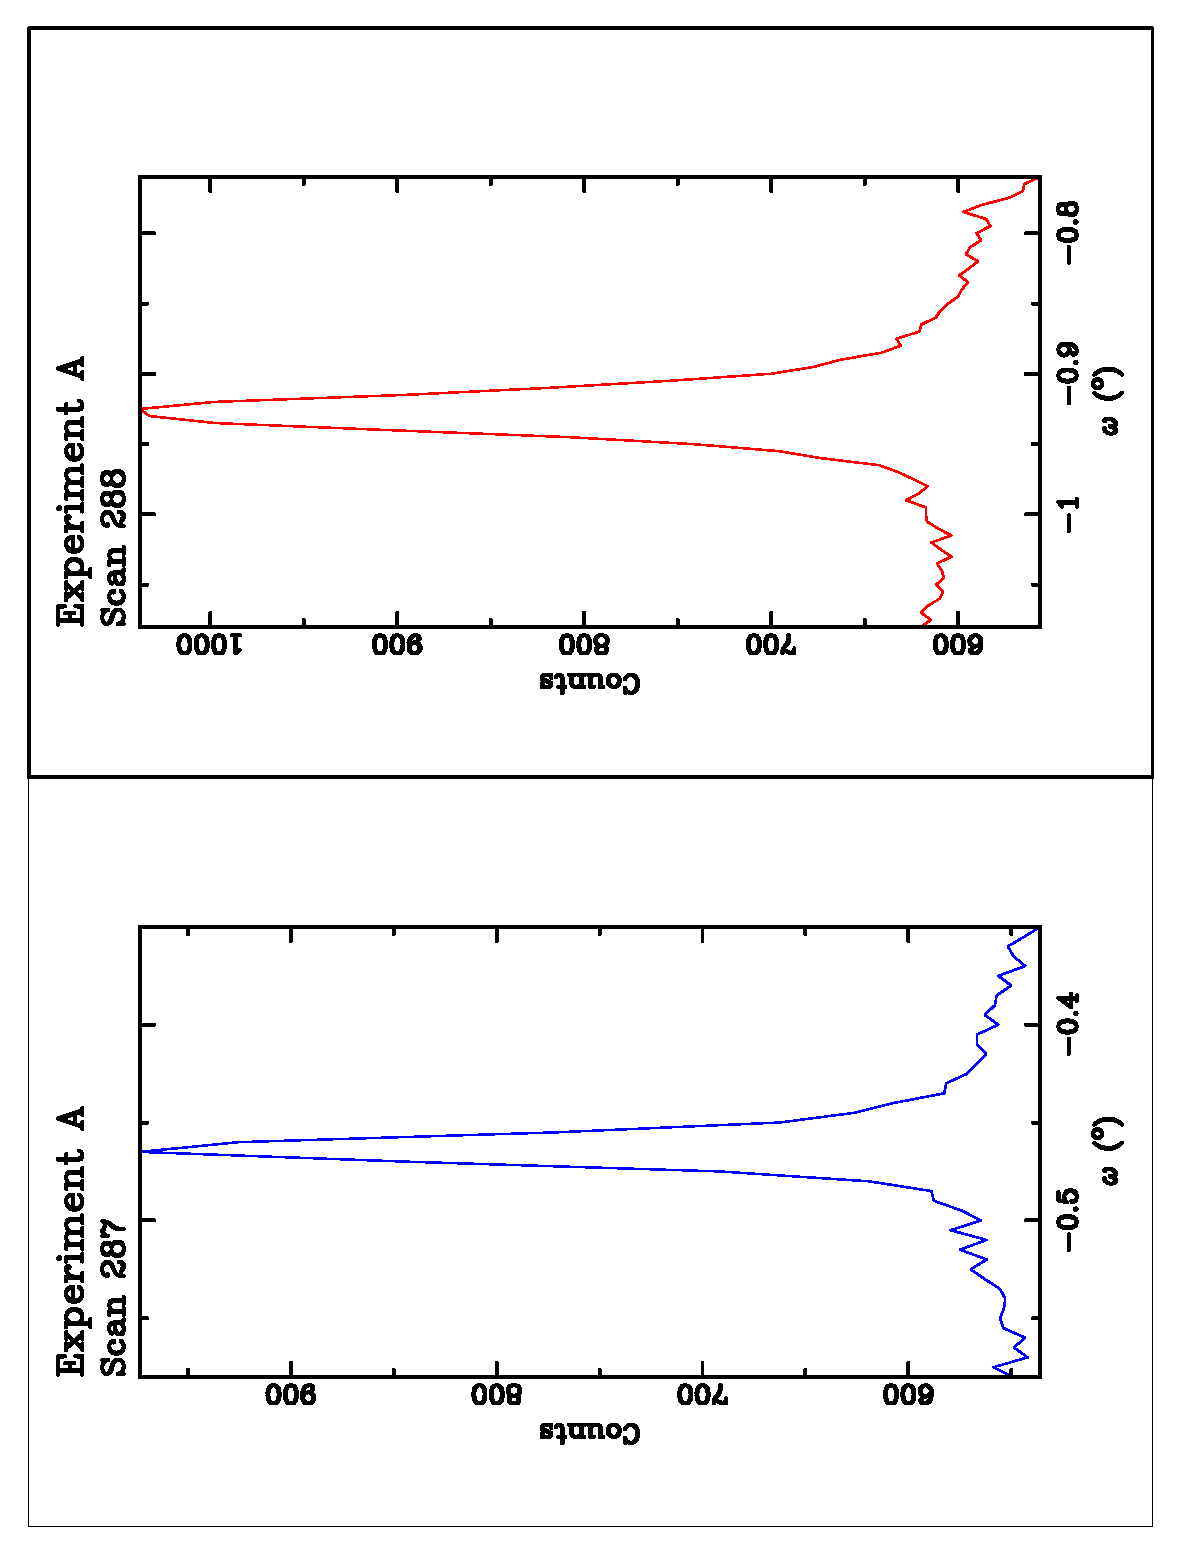
\includegraphics[scale=0.5, angle=270.0]{fra.1.eps}
   \caption{Simple example using frames}
   \label{fra-fig1}
\end{figure}

\begin{MacVerbatim}
     1  load xy,s287.xy
     2  load xy,s288.xy
     3  #
     4  tit1 Experiment A
     5  achx \gw (\uo\d)
     6  achy Counts
     7  mark 0.1,100
     8  buff 0.08
     9  fnam off
    10  fram on
    11  #
    12  nfra 2
    13  #
    14  afra 1
    15  kfra 1,1
    16  tit2 Scan 287
    17  #
    18  afra 2
    19  kfra 2,2
    20  tit2 Scan 288
    21  #
    22  plot
\end{MacVerbatim}

The macro starts with the reading of two data sets (lines 1--2).
Next title, axes labels and marker intervals are set (lines 4--7) as
in previous examples. The command 'buff' (line 8) alters the space
around the view graph reserved for axis numbering and titles. The
value is the fraction of the total width or height of the plot. In
our case we reserve 8\% of the page on all four sides of the plot as
buffer space. In line 9 the plotting of the filename is disabled and
in the following line the plotting of a border around each frame is
enabled. So far we have used no frame related commands and a plot at
this stage would show both data sets in a single view graph. In line
12 we then specify that we want to use two frames, i.e. have two
view graphs on our plot. At this stage, all settings from the
current plot (fram 1 in case we have used frames before) are copied
as defaults to all other frames. Entering command {\tt plot} now
would result in two equivalent view graphs side by side on the plot.
Thus all setting that are common to all frames should be made {\it
before} the command {\tt nfra} is used. Now we need to customize the
two frames. The command {\tt afra} determines for which frame the
following commands are used. First we alter settings for frame 1 by
entering {\tt afra 1} (line 14). Next we specify that this frame
should only contain the data from data set one (line 15) and we
enter an individual second title line (line 16). The same procedure
is repeated for frame 2 (lines 18--22) which should include data set
2 and a different subtitle line. The command {\tt plot} (line 22)
will result in a picture similar to the one in Figure
\ref{fra-fig1}.

\begin{table}[!tbh]
\centering
\begin{tabularx}{\textwidth}{|l|X|}
  \hline
  {\bf Command} & {\bf Description} \\
  \hline\hline
   afra & Sets the active frame for user input \\
   bfra & Sets background color for specified frame \\
   cfra & Copies frame parameters \\
   fram & Defines if a border is plotted around each frame \\
   kfra & Defines contents of frames (data sets or text) \\
   nfra & Sets number of frames (default = 1) \\
   sfra & Defines position and size of a frame \\
  \hline
\end{tabularx}
\caption{\label{fra-tab1}{\it KUPLOT} commands related to frames}
\end{table}

The usage of frames is rather simple and most {\it KUPLOT} settings
are individual settings for the different frames. All frame related
commands are summarized in table \ref{fra-tab1}. The following two
sections contain more complex examples using frames.

%------------------------------------------------------------------------

\section{Example 1: Using two different y-axes \label{frame-exa1}}

In this example, we will use frames to produce a plot that uses two
different y-axes to display two different data sets.  One y-axis
labeling will be on the left hand side of the view graph, the other
one on the right hand side.  The resulting plot is shown in figure
\ref{fra-fig2}. Here we display the scaling factor $f$ (right axis)
and the background parameter $b$ (left axis) of a Reverse Monte
Carlo refinement as function of the cycle number as an example plot.

\begin{figure}[!tb]
   \centering
   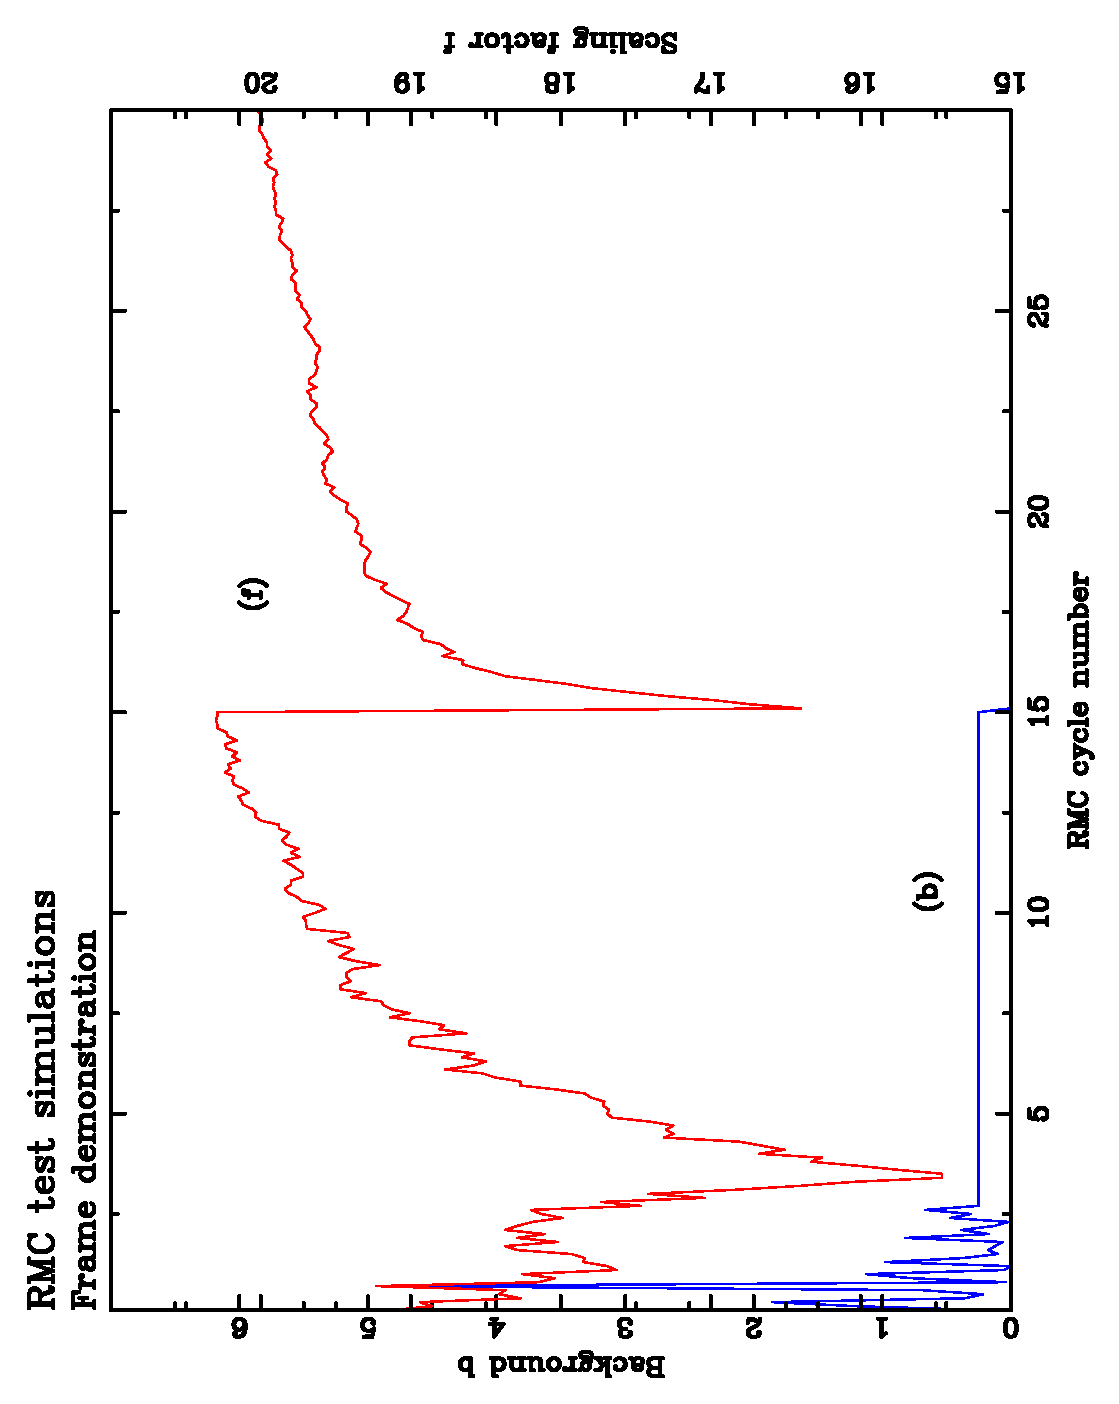
\includegraphics[scale=0.5, angle=270.0]{fra.2.eps}
   \caption{Using different y-axis with frames}
   \label{fra-fig2}
\end{figure}

We will discuss the corresponding macro file listed below step by
step. Again the line numbers are not actually part of the macro.
Lines 1--6 are nothing special, we read the two data files and set
common features like title lines.  Next we set the number of frames
to two (line 8). Since we want to plot the two data sets on top of
each other using just a different y-axes, we have to overwrite the
default location of the frames using the {\tt sfra} command (lines
10--11). The coordinates of the plot area range from 0.0 to 1.0 in
x- and y-direction. In our example both frames cover the complete
plot area.

\begin{MacVerbatim}
     1  load xy,back.xy
     2  load xy,scal.xy
     3  #
     4  fnam off
     5  tit1 RMC test simulations
     6  tit2 Frame demonstration
     7  #
     8  nfra 2
     9  #
    10  sfra 1,0.0,0.0,1.0,1.0
    11  sfra 2,0.0,0.0,1.0,1.0
    12  #
\end{MacVerbatim}

The next step is to input the settings for both frames. First we set
the input focus to frame 1 (line 13) and specify data set 1 to be
used in that frame (line 14). The {\tt fset} command in line 15
determines the layout of the view graph and setting number 3 is the
default plot layout, i.e. box, labels and tick marks in x- and
y-direction and lines at $x=0, y=0$. Finally we set the size of the
plotting window (line 16), the tick mark intervals (line 17) and the
labels for the axes (lines 18--19).

\begin{MacVerbatim}
    13  afra 1
    14  kfra 1,1
    15  fset 3
    16  skal 0.1,30.0,0.0,7.0
    17  mark 5.0,1.0
    18  achx RMC cycle number
    19  achy Background b
    20  #
\end{MacVerbatim}

The same as before has to be done for the second frame.  Lines
21--22 set the focus to the second frame and select data set 2 to be
displayed.  The negative value of the parameter of the {\tt fset}
command (line 23) indicates that the y-axis label and numbers are to
be plotted on the right hand side rather than on the left hand side
which is the default.  Again the extend of the plotting window and
the tick marks are set (lines 24--25).  Note that we need to specify
the same plotting range ($0.1 \rightarrow 30.0$) in x-direction and
a different one in y-direction compared to the settings of frame 1.
The x-axis label is switched off (line 26) because we have already
the label from the other frame.  The y-axis needs a new label (line
27).  Finally we define two annotations (line 28--29).  Note that
the given coordinates are with respect to the scaling of frame 2.

\begin{MacVerbatim}
    21  afra 2
    22  kfra 2,2
    23  fset -3
    24  skal 0.1,30.0,15.0,21.0
    25  mark 5.0,1.0
    26  achx
    27  achy Scaling factor f
    28  sann 1,"(b)",10.0,15.5
    29  sann 2,"(f)",17.5,20.0
    30  #
    31  plot
\end{MacVerbatim}

Obviously the same plot could have been achieved by scaling one of
the data sets to the y-range of the other, but the information about
the original range of y-values of one of the data sets would have
been lost in the plot in contrast to the example using frames given
here.

%------------------------------------------------------------------------

\section{Example 2: Connected view graphs \label{frame-exa2}}

In this section we will learn how we can create plots where several
graphs share one or more sides. This is done using the command {\tt
buff} we have used in the first part of this chapter. An example
plot is shown in Figure \ref{fra-fig3}.

\begin{figure}[!b]
   \centering
   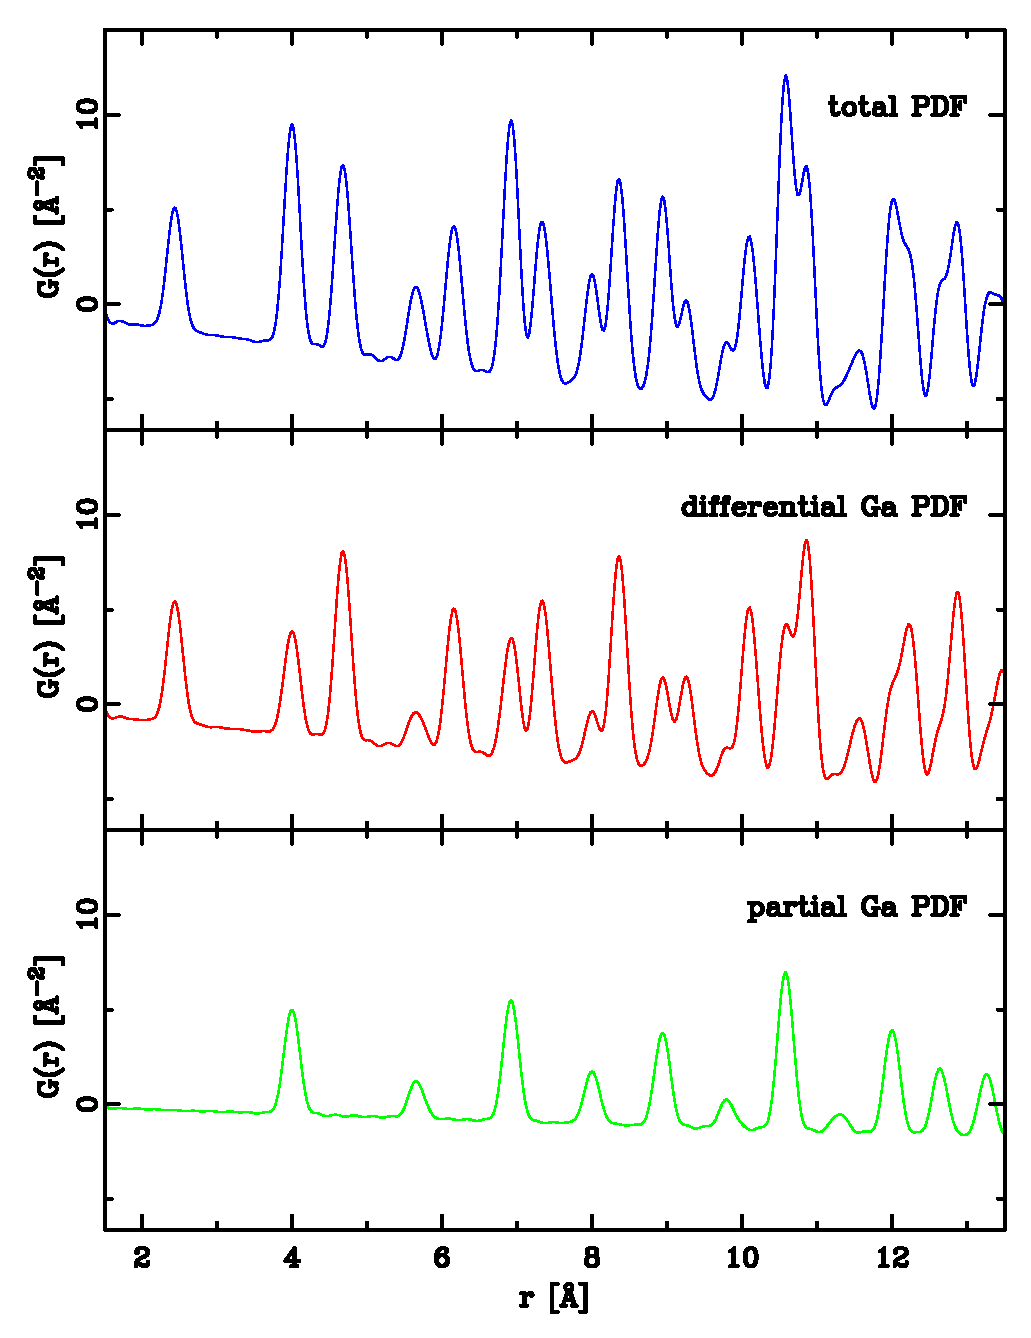
\includegraphics[scale=0.7, angle=0.0]{fra.3.eps}
   \caption{Example for connected view graphs}
   \label{fra-fig3}
\end{figure}

The macro used to create the plot is displayed below. As usual we start
resetting {\it KUPLOT} (line 1) and we select portrait orientation for
this plot (line 2). Next the data sets are loaded (lines 4--7).  This is
followed by general settings (lines 8--12) since all our frames will have
the save y-axis label, plot window and tick mark interval.

\begin{MacVerbatim}
      1  rese
      2  orient port
      3  #
      4  load xy,tot.calc
      5  load xy,dif_ga.calc
      6  load xy,par_ga.calc
      7  #
      8  fnam off
      9  fset 2
     10  achy G(r) [\A\u-2\d]
     11  skal xmin[1],xmax[1],1.2*ymin[1],1.2*ymax[1]
     12  mark 2.0,10.0
\end{MacVerbatim}

Next we define the frames, three on top of each other with no gap in
between them. Since the middle frame will have no buffer space on
the bottom and top we need to make it smaller in order for the plot
area to have the same size. Here we use variables for the task. The
value of the buffer size for title and axes labels is stored in {\tt
r[1]} (line 14), here 0.1. The remaining plot space for each panel
is calculated and stored in {\tt r[2]} (line 15). It is simply the
full size (1.0) minus two times the buffer size for the title of the
top panel and the axis label and numbering of the bottom panel. Next
we select three frames (line 17) and set the frame corners using the
variables we just defined. The $x$-range for all panels is 0.0 to
1.0. The $y$ ranges are determined by simply adding the heights of
the panels and the buffering space together (lines 18--20). Simply
calculate the numbers and it becomes clear.

\begin{MacVerbatim}
     13  #
     14  r[1] = 0.1
     15  r[2] = (1.0-2.0*r[1])/3.0
     16  #
     17  nfra 3
     18  sfra 1,0.0,2.0*r[2]+r[1],1.0,3.0*r[2]+2.0*r[1]
     19  sfra 2,0.0,    r[2]+r[1],1.0,2.0*r[2]+    r[1]
     20  sfra 3,0.0,0.0          ,1.0,    r[2]+    r[1]
\end{MacVerbatim}

In the next section the setting for the individual frames are
entered. Most of the commands were already discussed in the previous
chapters. The command {\tt buff} can either be used with a single
parameter like in the example in section \ref{frame-int} in which
case the buffer space around the view graph is the same in all
directions. Alternatively one can supply four parameters for the
required free space on the left and right side and the bottom and
top of the view graph, respectively. In our example this first frame
located on the top will have no buffer space at the bottom (line
23). Apparently we have to turn the numbering for the x-axis off
(line 25). Now we repeat the settings for the other two frames. For
the middle frame we have no buffer space on the top an bottom (line
29) and for the bottom frame we have only buffer space at the bottom
(line 34). Also we need to set a x-axis label for the bottom panel
(line 38).

\begin{MacVerbatim}
     21  #
     22  afra 1
     23  buff 0.1,0.1,0.0,r[1]
     24  kfra 1,1
     25  achx OFF
     26  sann 1,"total PDF",13.0,10.0,right
     27  #
     28  afra 2
     29  buff 0.1,0.1,0.0,0.0
     30  kfra 2,2
     31  achx OFF
     32  sann 1,"differential Ga PDF",13.0,10.0,right
     33  #
     34  afra 3
     35  buff 0.1,0.1,r[1],0.0
     36  kfra 3,3
     37  sann 1,"partial Ga PDF",13.0,10.0,right
     38  achx r [\A]
\end{MacVerbatim}

Frames are a flexible tool and can be placed anywhere on the plot
area and may also overlap. A even slightly more complex example using
frames is discussed in the next section.

%------------------------------------------------------------------------

\section{Example 3: Advanced frame usage \label{frame-exa3}}

The final example for the usage of frames is more complex and the
resulting plot is shown in Figure \ref{fra-fig4}. {\it KUPLOT} is
capable of creating quite complex plots and e.g. allows one to create
complete transparencies for a talk.

\begin{figure}[!p]
   \centering
   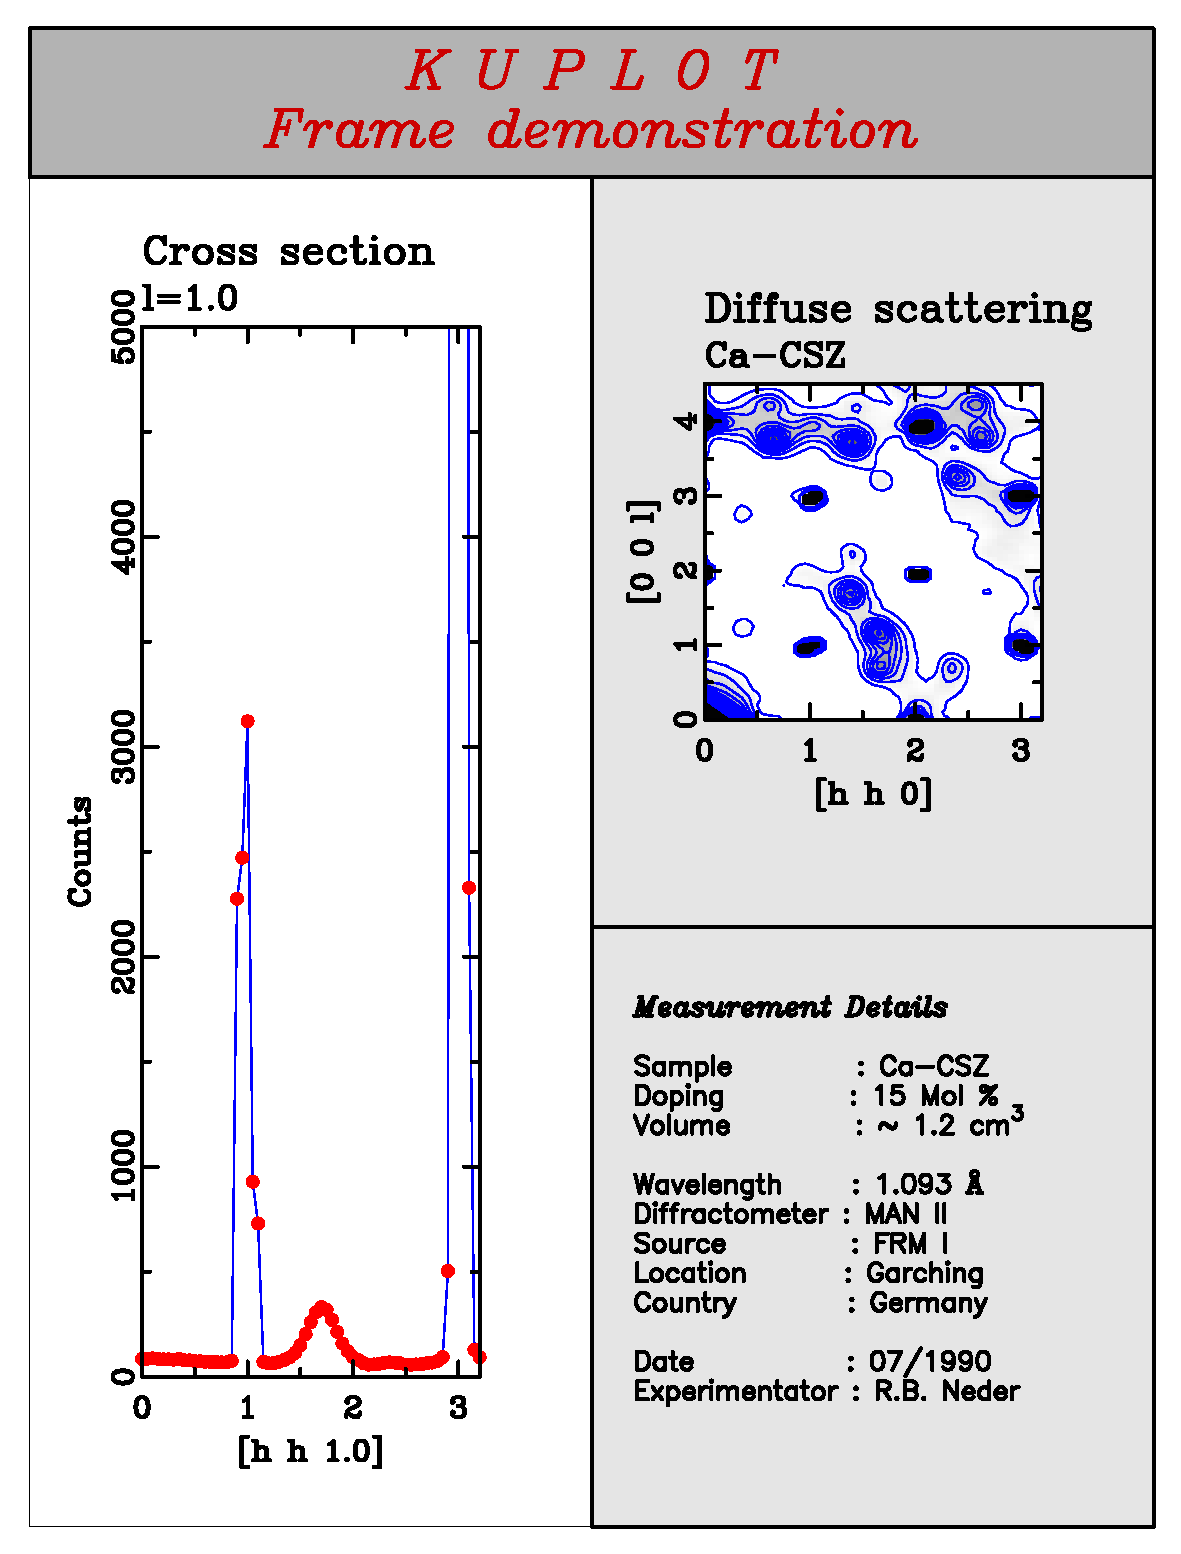
\includegraphics[scale=0.75]{fra.4.eps}
   \caption{Advanced frame example plot}
   \label{fra-fig4}
\end{figure}

The macro used to create the plot is displayed below. As usual the
data sets are loaded first (lines 1--2) followed by general
settings (line 4). Next we select 4 frames (line 6) and define the
desired frame layout (lines 8--11) and individual background
colors for each frame (lines 13--15). Note that the default
background color is white. The colors are given as RGB (red,
green, blue) values ranging from 0.0 to 1.0.

\begin{MacVerbatim}
     1  load xy,test.cut
     2  load ni,test.nipl
     3  #
     4  fnam off
     5  #
     6  nfra 4
     7  #
     8  sfra 1,0.0,0.0,0.5,0.9
     9  sfra 2,0.5,0.4,1.0,0.9
    10  sfra 3,0.5,0.0,1.0,0.4
    11  sfra 4,0.0,0.9,1.0,1.0
    12  #
    13  bfra 2,0.9,0.9,0.9
    14  bfra 3,0.9,0.9,0.9
    15  bfra 4,0.7,0.7,0.7
\end{MacVerbatim}

The next part of the macro file contains the settings for frame 1.
After setting the focus to this frame (line 19), data set 1 is
selected for this frame (line 20). The following commands specify
various settings and were already explained in previous examples.
The {\tt font} command in line 32 increases the font size of all
fonts used for this frame by 10\%.

\begin{MacVerbatim}
    16  #
    17  # Frame 1 with cross section
    18  #
    19  afra 1
    20  kfra 1,1
    21  buff 0.4
    22  lcol 1,6
    23  mtyp 1,3
    24  mcol 1,1
    25  msiz 1,0.2
    26  skal 0.0,3.2,0.0,5000.0
    27  mark 1,1000
    28  achx [h h 1.0]
    29  achy Counts
    30  tit1 Cross section
    31  tit2 l=1.0
    32  font size,1.1
\end{MacVerbatim}

Next we have the settings for frame 2 containing the 2D data set
number 2, the diffuse neutron scattering of Ca-CSZ we used as example
before. Again the various commands were  explained in earlier examples.

\begin{MacVerbatim}
    33  #
    34  # Frame 2 with data plot
    35  #
    36  afra 2
    37  kfra 2,2
    38  glat 2,3
    39  hart 2,3
    40  hcol 2,1,3
    41  hlin 1,100,50,12
    42  mark 1,1,0,0
    43  aver 0.707
    44  achx [h h 0]
    45  achy [0 0 l]
    46  tit1 Diffuse scattering
    47  tit2 Ca-CSZ
    48  font size,1.1
\end{MacVerbatim}

The next frame contains text rather than data.  The text for this
frame is read from the file {\it ref.txt} which contains exactly the
text you can see at the bottom right corner of the plot in Figure
\ref{fra-fig4}.  In lines 52--56 the justification of the text, the
font type and font size are specified. The text file may contain the
same special characters and control sequences discussed in section
\ref{1d-char}.

\begin{MacVerbatim}
    49  #
    50  # Frame 3 with text
    51  #
    52  afra 3
    53  kfra 3,ref.txt
    54  font just,left
    55  font typ,5,1
    56  font siz,5,12
\end{MacVerbatim}

Finally we specify another text file containing the title line of
the plot. We select the text to be centered (line 62) and set the
font to {\it italics} (font 3), set the color to dark red (pen 7)
and increase the size of the font to 24 points.

\begin{MacVerbatim}
    57  #
    58  # Frame 4 with title text
    59  #
    60  afra 4
    61  kfra 4,tit.txt
    62  font just,center
    63  font typ,5,3
    64  font col,5,7
    65  font siz,5,24
\end{MacVerbatim}

Currently one has not much control about the layout in a frame containing
text but that might change in future version of the program {\it KUPLOT}.

%------------------------------------------------------------------------

%------------------------------------------------------------------------
% Chapter:  Using the mouse
%------------------------------------------------------------------------

\chapter{Using the mouse \label{mouse}}

%------------------------------------------------------------------------
\section{Mouse interface \label{mouse-interface}}

To enter the mouse mode, simply use the command {\tt mouse}. The
plot window will now contain a number off buttons in addition to the
view graph as can be seen in Figure \ref{mou-fig1}.
%
\begin{figure}[!b]
   \centering
   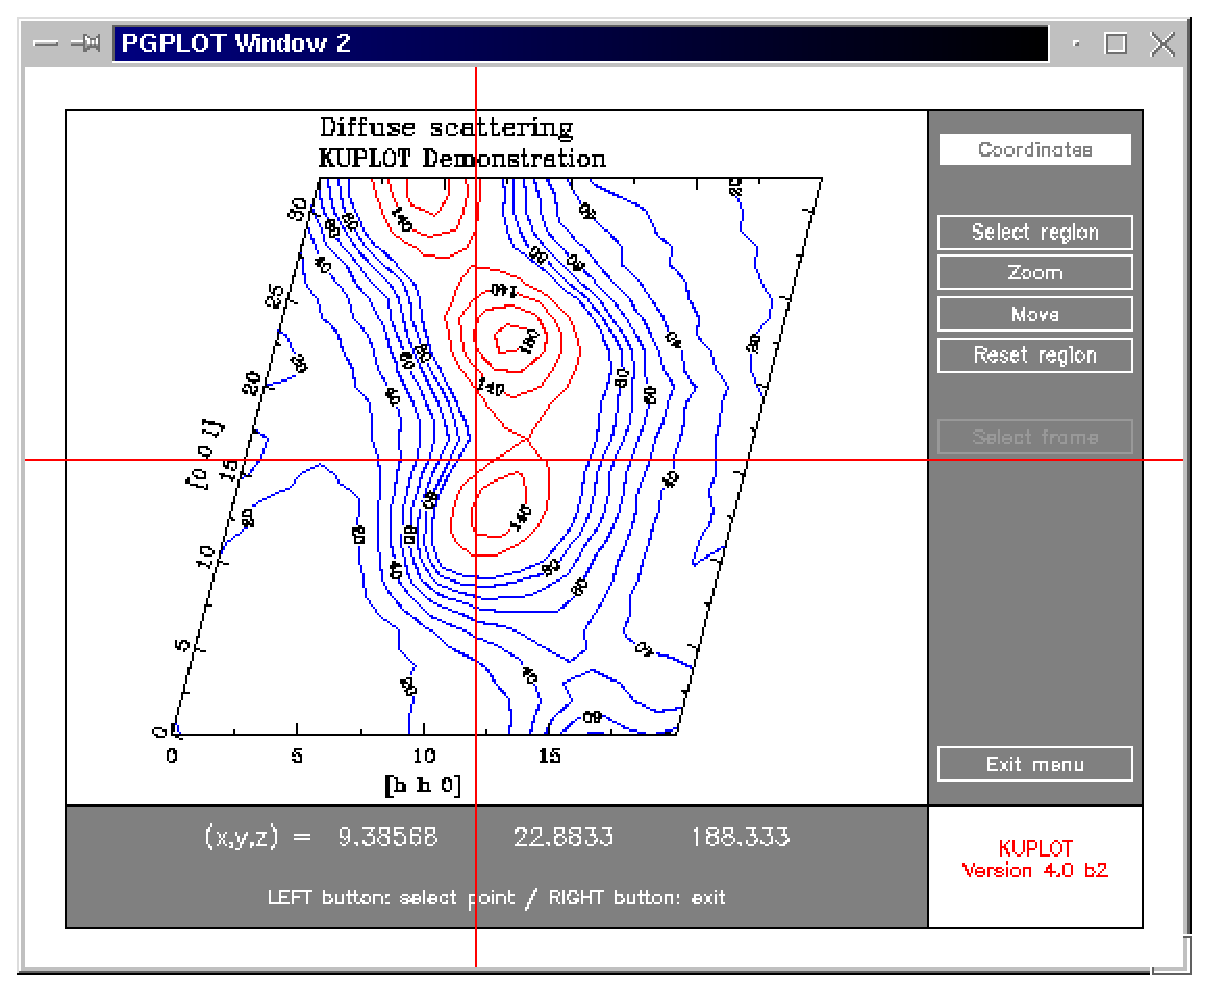
\includegraphics[scale=0.5]{mou.1.eps}
   \caption{{\it KUPLOT} in {\it mouse} mode}
   \label{mou-fig1}
\end{figure}
%
The button {\it Coordinates} allows the user to display the
coordinates of the mouse pointer by clicking the left mouse button.
The values are displayed below the plot. In case of 2D files, the
$z$-value of the closest data point is also shown. The right mouse
button terminates the coordinate display function. The next group of
buttons allows the user to use the mouse to modify the potting area.
{\it Select region} does exactly that by clicking on the lower left
corner of the desired area first. A moving frame will appear and the
user can select the other corner of the new region. The buttons {\it
Zoom} and {it Move} perform these functions using all three mouse
buttons. A short help text explaining which button is doing what
appears below the plotting area once a function is selected. 'Reset
region' allows the user to quickly display the complete range of
data again. In cases where the current plot contains frames (see
chapter \ref{frame}), the active frame is marked by a light red
background color. All functions will affect the active frame only.
The focus can be moved to another frame via the {\it Select frame}
button, which is only active when there is more than a single frame.
Finally to get back to the command prompt of {\it KUPLOT} use the
{\it Exit menu} button. Note that in cases where commands are
written to a macro file via the command {\tt learn}, all region
functions will write the corresponding {\tt skal} command in the
macro file. One should also be careful when using the {\tt mouse}
command in macro files, since {\it KUPLOT} will not execute any
further commands in until the {\it Exit menu} button is hit.
\par

%------------------------------------------------------------------------
\section{Mouse in macros \label{mouse-mac}}

In the previous section, we learned about the interactive interface
of {\it KUPLOT}. Alternatively, the {\tt mouse} command can have
additional parameters which specify what will be selected using the
mouse pointer. In this case no buttons will show up and the
coordinates will be returned in the {\tt res[]} variables. Let us
consider the following example. The goal is to use the mouse to
select a number of points and store those in a data set. This could
e.g. be used to define a background underneath some data manually.
The macro file is show here:
%
\begin{MacVerbatim}
    1  variable integer,pt
    2  variable integer,npt
    3  variable integer,button
    4  #
    5  npt=0
    6  button=0
    7  #
    8  echo Select points - right mouse button to finish
    9  #
   10  do while (button.ne.3)
   11    mouse point
   12    npt=npt+1
   13    r[100+npt]=res[1]
   14    r[200+npt]=res[2]
   15    button=res[3]
   16  enddo
   17  #
   18  npt=npt-1
   19  alloc back,npt
   20  do pt=1,npt
   21    x[n[1],pt]=r[100+pt]
   22    y[n[1],pt]=r[200+pt]
   23  enddo
   24  #
   25  plot
\end{MacVerbatim}
%
We assume the data set of interest has been loaded and one has
zoomed into the area where the background should be defined. In
lines 1--3 we define the required variables. Note that this uses the
new feature of named variables discussed in more detail in chapter
\ref{fort}. In lines 5 and 6 some variables are initially set to
zero. In line 8 a message is printed on the screen to tell the user
what to do. Basically every left click with the mouse will define a
point and a right click will exit the macro and store the selected
points. In line 10 we start a {\tt while} loop which is executed
until the variable {\tt button} contains the number 3 which
corresponds to the clicking the right mouse button. The command {\tt
mouse point} allows the user to select a point. The coordinates and
the button pressed are returned in variables {\tt res[i]} and are
stored in variables (lines 13--15). This loop is now repeated until
the right mouse button is pressed. Every time the variable {\tt npt}
is incremented, containing the number of points selected so far. The
way the loop is constructed, {\tt npt} actually contains the number
of points plus on which is fixed in line 18. The command {\tt alloc}
(line 19) now creates a new and empty {\it KUPLOT data set} with a
size of {\tt npt} points. The loop in lines 20--23 is then used to
store the coordinates selected in that data set and finally the data
and background data set are plotted (line 25). In reality one would
add commands to either interpolate and subtract the background
directly or store it in a data file. The command {\tt mouse} can
also be used to select a region or range (see Table \ref{mou-tab1}).

%
\begin{table}[!t]
\centering
\begin{tabularx}{\textwidth}{|p{15mm}|X|}
  \hline
  {\bf Mode} & {\bf Description} \\
  \hline\hline
  point   & Selects a single point and returns $x,y$ or $x,y,z$ in
            variable {\tt res[i]}.\\
  line    & Selects two points connected by a line.\\
  rect    & Selects two corners of a rectangle.\\
  xrange  & Selects two points defining range in $x$.\\
  yrange  & Selects two points defining range in $y$.\\
  \hline
\end{tabularx}
\caption{\label{mou-tab1}Modes of command {\tt mouse}}
\end{table}
%

%------------------------------------------------------------------------

%------------------------------------------------------------------------
% Chapter:  Mathematics
%------------------------------------------------------------------------

\chapter{Manipulating and analyzing data \label {mat}}

In this chapter we will discuss {\it KUPLOT} functions that allow the
analysis and manipulation of data. The first two sections deal with
data manipulation, first using build-in functions and later using
variables. The last section of this chapter summarizes data analysis
functions of {\it KUPLOT}.

%------------------------------------------------------------------------

\section{Simple data calculations \label{mat-buildin}}

A common task is the numerical manipulation of a data set, e.g.  to
add some constant to a data set or inverse all y-values.  The
command {\tt ccal} offers a variety of manipulation functions for a
specific data set.  The command {\tt kcal} on the other had allows
simple arithmetic operations between two data sets.  The commands
and valid operations are listed in Table \ref{mat-tab1}.

\begin{table}[!b]
\centering
\begin{tabular}{|l|c|l|}
  \hline
  {\bf Command} & {\bf Operation} & {\bf Description} \\
  \hline\hline
   ccal & abs & Performs $x_{i} = |x_{i}|$ \\
        & add & Performs $x_{i} = x_{i} + a$ \\
        & exp & Performs $x_{i} = \exp (x_{i})$ \\
        & inv & Performs $x_{i} = \frac {1} {x_{i}}$ \\
        & log & Performs $x_{i} = \ln  (x_{i})$ \\
        & mul & Performs $x_{i} = f \cdot x_{i}$ \\
        & sqr & Performs $x_{i} = \sqrt {x_{i}}$ \\
        & squ & Performs $x_{i} = x_{i}^{2}$ \\
  \hline
  kcal  & add & Performs $x'''_{i} = x''_{i} + x'_{i}$ \\
        & sub & Performs $x'''_{i} = x''_{i} - x'_{i}$ \\
        & mul & Performs $x'''_{i} = x''_{i} \cdot x'_{i}$ \\
        & div & Performs $x'''_{i} = x''_{i} / x'_{i}$ \\
  \hline
\end{tabular}
\caption{\label{mat-tab1}Data manipulation functions}
\end{table}

Note that $x_{i}$ in Table \ref{mat-tab1} stands for x-, y-, z- and
$\sigma_{x}$- or $\sigma_{y}$-values depending on the given parameters.
The following simple command will multiply all y-values of data set one
with the factor 1.75:
%
\begin{MacVerbatim}
     ccal mul,wy,1,1.75
\end{MacVerbatim}
%
The parameter {\tt mul} indicates that a multiplication is to be
performed using the y-values which are selected by the next
parameter ({\tt wy}). Finally data set one and the desired factor of
1.75 are specified. For x- and z-values use {\tt wx} and {\tt wz},
the standard deviations $\sigma_{x}$ and $\sigma_{y}$ are selected
using the parameters {\tt dx} and {\tt dy}.

%------------------------------------------------------------------------

\section{Calculating functions \label{mat-func}}

Another feature of {\it KUPLOT} is the capability to create a data
set from an arithmetic expression rather than reading it from a
file. This is done using the command {\tt func}. The following two
commands demonstrate usage of {\tt func} to create a 1D data set ($y
= \sin(x))$ and a 2D data set ($z = \sin(x) \cdot \cos(y))$.
%
\begin{MacVerbatim}
   func sin(r[0]),0.0,6.3,0.1
   func sin(r[0])*cos(r[1]),0,6,0.1,0,6,0.1
\end{MacVerbatim}
%
Note that the variable {\tt r[0]} is used for the x-argument and
{\tt r[1]} is used as y-argument. Thus values previously stored in
these two variables are destroyed by the {\tt func} command. The
following commands are the range and the grid size in the two
directions. In our first example, the desired x-range is $0.0
\rightarrow 6.3$ with a grid size of $\Delta x = 0.1$. This results
the creation of a data set with 64 points. The second {\tt func}
command shown above creates a 2D data set ranging from 0.0 to 6.1 in
x- and y-direction with a grid size of $\Delta x = \Delta y = 0.1$
given a size of 61x61 data points. Alternatively, space for a new
data set can be initialize using the command {\tt alloc} and the
data values are then calculated using the FORTRAN style interpreter
of {\it KUPLOT} (see section \ref{mat-var}). However,  the creation
of large data sets this way from an arithmetic expression might be
relatively slow. \par

%------------------------------------------------------------------------

\section{Data manipulation \label{mat-man}}

\subsection{Data smoothing \label{mat-smooth}}

\begin{figure}[!ptb]
   \centering
   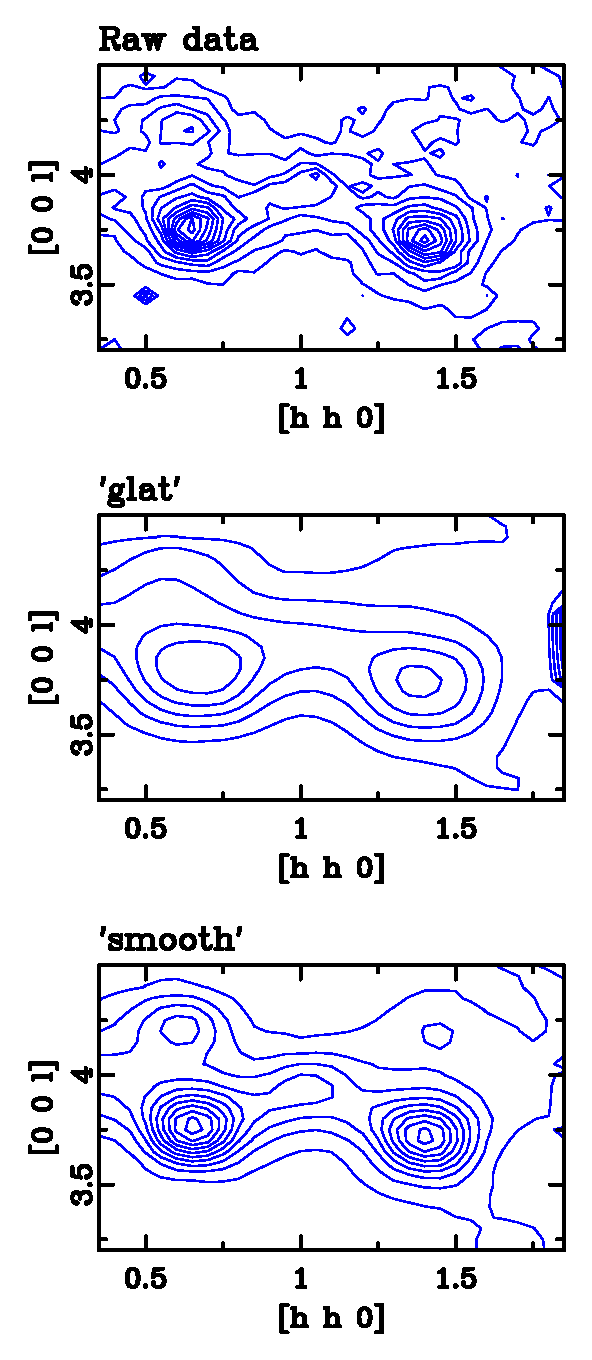
\includegraphics[scale=0.8]{mat.1.eps}
   \caption{Demonstration of data smoothing}
   \label{mat-fig1}
\end{figure}

{\it KUPLOT} has two different smoothing functions that can be used
for 1D as well as 2D data. The first type of smoothing is a simple
sliding average. The corresponding command is {\tt glat}. The name
is a reminder that the first {\it KUPLOT} version was in German
(smoothing in German is gl\"atten). The smoothing is performed by a
sliding average of $n$ neighboring points. The value of $n$ is given
as parameter of the command {\tt glat}. An example for the smoothing
operation is given in Figure \ref{mat-fig1}. The top view graph
shows the raw data showing quite noisy contour lines. The picture
below shows the same data after the data set was smoothed with a
value of $n=7$ using the command {\tt glat 1,7} assuming the values
are stored as data set one. It is apparent from Figure
\ref{mat-fig1} that this type of averaging broadens the peaks and
does not preserve the peak heights. An alternative way to smooth
data implemented in {\it KUPLOT} is the Savitzky-Golay algorithm
which is in principle a weighted sliding average. The weight is
given by a polynomial of user definable order (the default is 2).
The command for the later type of smoothing is {\tt smooth} with
parameters identical to {\tt glat}. However, the minimum number of
$n$ is five. The bottom view graph in Figure \ref{mat-fig1} was
smoothed with $n=7$ using the command {\tt smooth}. It can be
clearly seen that the widths and heights of the peaks are much
better preserved. For a detailed discussion about the smoothing
algorithm and its limits see e.g. Numerical Recipes by Press,
Flannery, Teukolsky \& Vetterling, Cambridge University Press, 1989.
\par

As a default, 2D data sets are per smoothed in x and y direction.
The user can restrict the smoothing to only one direction by adding
the optional parameter {\tt x} or {\tt y} to the {\tt glat} or {\tt
smooth} command. Again the reader might refer to the online help for
more detailed information on the smoothing commands.


\subsection{Sorting data \label{mat-sort}}

The command {\tt sort ik} will sort the data points in data set {\tt
ik} by increasing $x$ values. No other sorting is currently
implemented in {\it KUPLOT}, however one might implement any sorting
algorithm using the FORTRAN interpreter of the program.


\subsection{Rebinning data \label{mat-rebin}}

Sometimes a data set needs to be transformed onto a different grid
of $x$ or $x,y$ values. This is usually referred to as rebinning.
The most common application is to transform a data et from an
irregular grid to an equidistant grid. {\it KUPLOT} offers a
different mechanism for 1D and 2D data sets. The command {\tt rebin
ik, delta} will rebin the 1D data set {\it ik} to an equidistant
grid with a bin width of {\tt delta}. One needs to take care, that
the new grid is at least slightly larger than the original to
prevent 'holes' from appearing. In addition to an equidistant grid,
a data set can be interpolated on a set of $x$ values given by a
different data set. The command {\tt spline 1,2} for example would
interpolate data set one onto the $x$ values given by data set 2 and
store the result in a new data set.\par

To rebin a 2D data set, one needs to first save it in $x,y,z$ or
{\tt gn} format. This data file is then load back into {\it KUPLOT}
using the command {\tt load zz,file,dx,dy} and rebinned on the
desired grid {\tt dx, dy}. Obviously one can load $x,y,z$ files on
an irregular grid the same way. \par


\subsection{Matching and merging data sets \label{mat-merge}}

Sometimes two data sets differ by a scaling factor of an offset. The
command {\tt match} allows to find the scaling and/or offset that
gives the best agreement between two data sets. The scaling and
background is directly applied. Note that this function only works
for data sets, that have identical points in $x$. The command {\tt
merge} allows one to combine data sets. Points with common
$x$-values are averaged.

%------------------------------------------------------------------------

\section{Data manipulation using variables \label{mat-var}}

A very flexible way to manipulate data is the use of variables.
Details about the FORTRAN style interpreter and the usage of
variables were discussed in chapter \ref{fort}. Two simple examples
are given here for illustration. \par

In the first example we assume having a data set containing measured
intensities as function of some angle $\omega$. The following {\it
KUPLOT} commands will create values for $\sigma_{y}$ according to the
relation $\sigma_{y}(i) = \sqrt{y(i)}$.

\begin{MacVerbatim}
     1  do i[1]=1,np[1]
     2    dy[1,i[1]]=sqrt(y[1,i[1]])
     3  enddo
\end{MacVerbatim}

The first line starts a DO loop over all data points of data set
one, assuming that is where our data are stored. The variable {\tt
i[1]} is the loop control variable and {\tt np[1]} contains the
number of data points of data set one. For a complete list of
variables refer to section \ref{var} of this users guide. Next the
value of $\sigma_{y}$ for data point i[1] is computed (line 2). The
first parameter in {\tt dy[1,i[1]]} specifies data set one. Finally
(line 3) the loop is closed. The corresponding plot with the error
bars of the newly created values of $\sigma_{y}$ is shown in Figure
\ref{mat-fig2}.

\begin{figure}[!t]
   \centering
   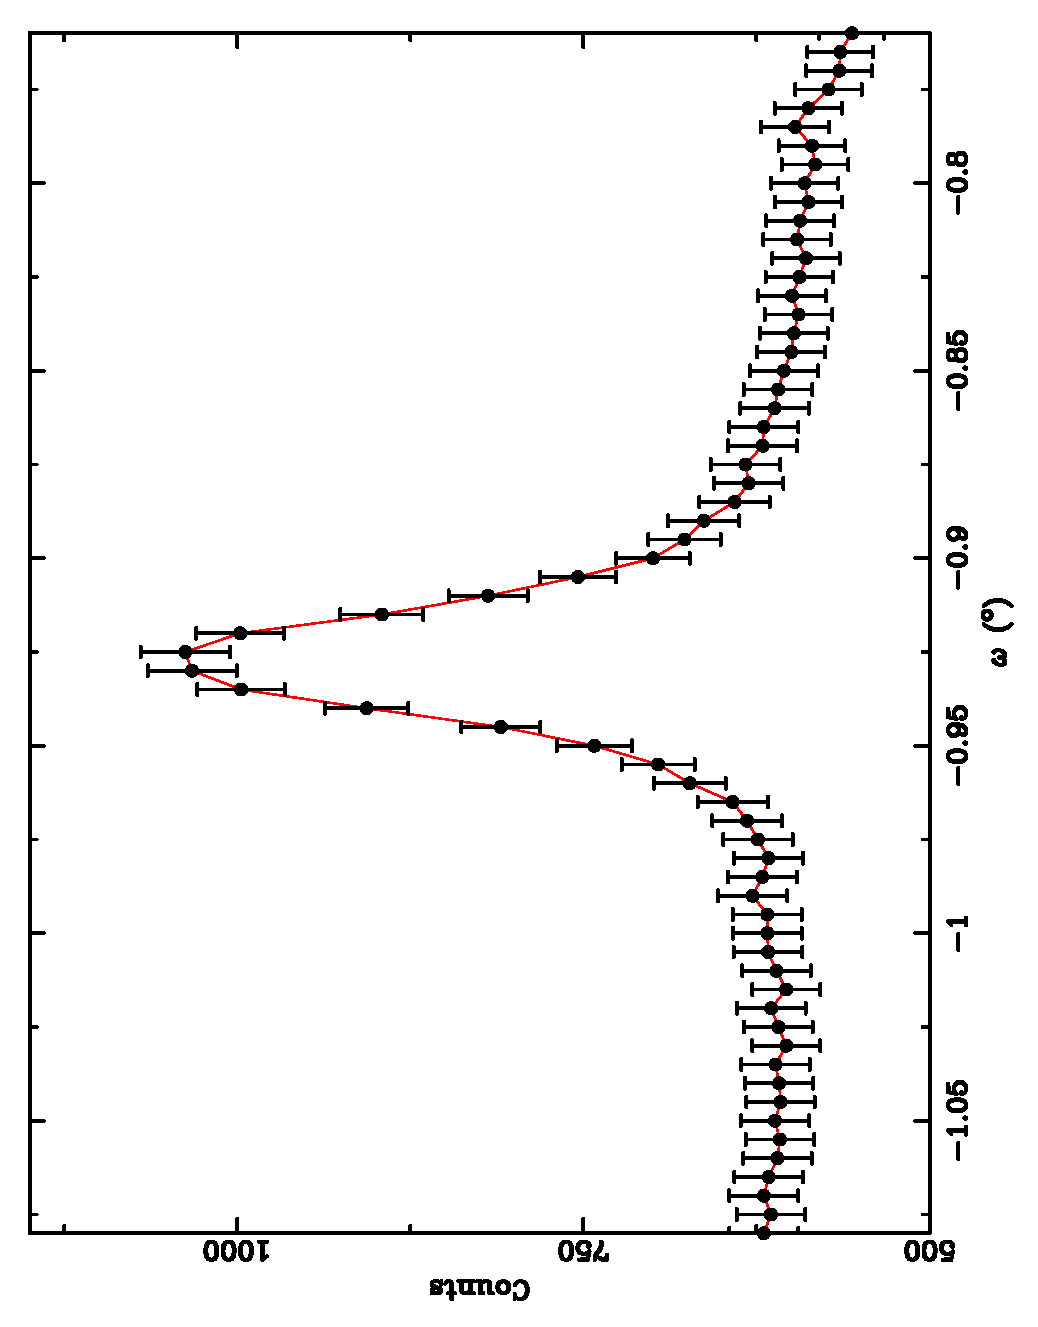
\includegraphics[scale=0.5, angle=270.0]{mat.2.eps}
   \caption{Plot of data manipulation example}
   \label{mat-fig2}
\end{figure}

The second example shows how to create a new data set using variables.
We assume that we have two data sets loaded, both having the same length
and identical x-values. We want to create a new data set with
the same x-values and y-values that are the average of the y-values of
the two load data sets, thus $y_{i}'''=\frac{1}{2}(y_{i}''+y_{i}')$.
Here $y'''$ stands for the new data set whereas $y''$ and $y'$
represent the values of the two loaded data sets. The {\it KUPLOT}
commands for our task are listed below:

\footnotesize
\begin{MacVerbatim}
     1  alloc aver.xy,np[1]
     2  #
     3  do i[1]=1,np[1]
     4    x[3,i[1]]=x[1,i[1]]
     5    y[3,i[1]]=0.5*(y[1,i[1]]+y[2,i[1]])
     6  enddo
\end{MacVerbatim}
\normalsize

First we have to allocate space for the new data set. This is
normally done by the command {\tt load} or {\tt func}, but the
command {\tt alloc} allows the user to create an empty data set,
just what we need here. The name {\it aver.xy} given as parameter to
the {\tt alloc} command in line 1 is the internal name for the data
set, e.g. showing up in the top left corner of the plot or when
using the {\tt show} command. This is an arbitrary name and {\bf no}
file of that name needs to exist. The second parameter specifies the
size of the new data set, in out case the same size as data sets one
(variable {\tt np[1]}) or two. Next we have a loop as in the
previous example over all data points (line 3). In lines 4--5 the
$x$- and $y$-values of the new data set number 3 are computed. Since
we assumed that both original data sets have the same $x$-values, we
just use one of them as $x$-values for the new set. Finally the loop
is closed (line 6).
\par

Although the usage of variables allows one to perform the same
functions as the {\tt ccal} and {\tt kcal} commands, the usage of
variables is much slower especially for large data sets and should
only be used if no corresponding build-in function is available.

%------------------------------------------------------------------------

\section{Data analysis \label{mat-anal}}

This section describes the data analysis functions of {\it KUPLOT}.
Apparently variables can also be used to calculate averages and
analyze data sets. The contents of a variable or result of an
expression can be displayed with the command {\tt eval}. Another
wide area of data analysis is to fit a theory function to a data
set. The least square fitting functions of {\it KUPLOT} are
discussed in the next chapter. As example for this chapter we use a
subsection of the diffuse scattering data displayed in previous
examples. The data are shown in Figure \ref{mat-fig3}. The circles
mark positions of maxima found in the data set by the command {\tt
smax}.

\begin{figure}[!t]
   \centering
   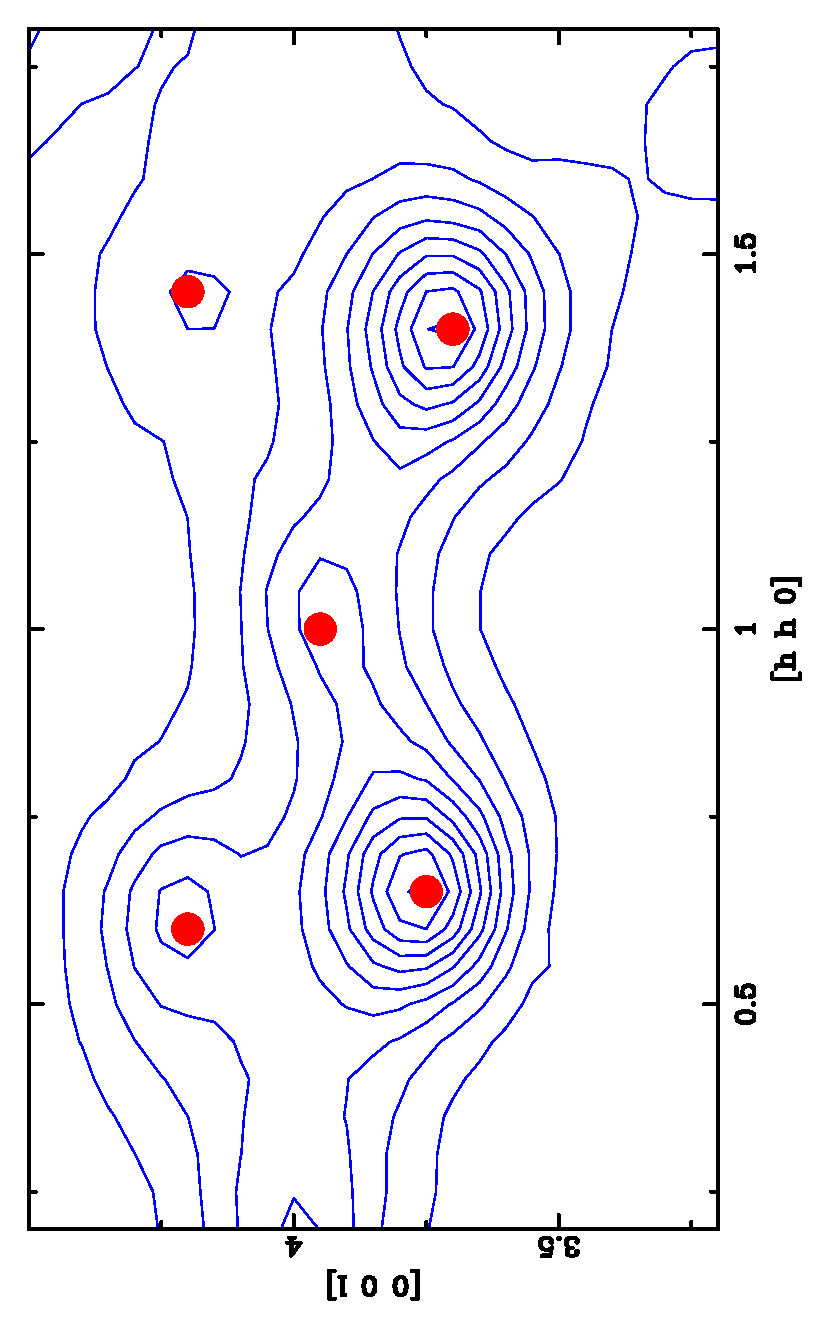
\includegraphics[scale=0.4, angle=270.0]{mat.3.eps}
   \caption{Marking of maxima within a plot}
   \label{mat-fig3}
\end{figure}

A maximum determined by {\tt smax} is defined as a point where all
$n$ neighboring points have smaller $y$- or $z$-values compared to
the reference point. The value of $n$ is the second parameter of the
{\tt smax} command, the first is the data set number. The maxima
marked in Figure \ref{mat-fig3} were determined with {\tt smax 1,3}
assuming we are dealing with data set one. The command {\tt ptyp}
allows one to select a symbol analog to {\tt mtyp} to mark the
positions of the determined maxima. Furthermore the positions of the
found maxima are displayed on the screen. The output for our example
is shown below:

\begin{MacVerbatim}
   Found maxima data set   1 (ifen =   3) :

      No.        pos. x       pos. y         value
      --------------------------------------------------
        1         .600        4.200             272.778
        2         .650        3.750             567.111
        3        1.000        3.950             273.889
        4        1.400        3.700             509.667
        5        1.450        4.200             156.778
\end{MacVerbatim}

You might verify these coordinates as the marked positions in figure
\ref{mat-fig3}. Other functions allow the user to determine the
integral or mean values of a given area of the data set.\par

Next we will determine the integral of the left diffuse peak in
figure \ref{mat-fig3}. This is done using the command

\begin{MacVerbatim}
    inte 1, .423750, .903750, 3.4716, 3.99168
\end{MacVerbatim}

The first parameter specifies the data set number followed by the area
to be integrated given as $x_{min}, x_{max}, y_{min}$ and $y_{max}$.
If those last 4 parameters are omitted, the complete current plotting
window is used. The screen output of this command is:

\footnotesize
\begin{MacVerbatim}
    Integration result for data set   1 :
       x-range    :    .4238     to    .9038
       y-range    :    3.472     to    3.992
       Integral   :    57.06     +-    .3650      (    100 pkt)
\end{MacVerbatim}
\normalsize

The command {\tt mean} with similar parameters can be used to
calculate mean values and standard deviations in the given region.
The region above was determined using the {\tt mouse} functions (see
\ref{mouse}).

%------------------------------------------------------------------------

\section{Fourier transform \label{mat-four}}

{\it KUPLOT} can calculate a discrete Fourier transform of a 1D or
2D data set. Let us start with a little mathematics first. Details
can again be found in the Numerical Recipes. The function we want
to Fourier transform is $f(x_{i})$ with $i=1,..N$ with a constant
grid size of $\Delta x$. This gives us the following range in Fourier
space:

\begin{equation}
  h_{n} = \frac{n}{N \Delta x} \;\; \mbox{with} \;\;
      n = -\frac{N}{2} .. \frac{N}{2}
  \label{mat-eq1}
\end{equation}

\noindent
The Fourier transform is calculate as

\begin{equation}
  F(h_{n}) = \Delta x \sum_{i=1}^{N} f(x_{i}) \left [
             \cos (2\pi h_{n}x_{i}) + i \sin (2\pi h_{n}x_{i}) \right ].
  \label{mat-eq2}
\end{equation}

\begin{figure}[!t]
   \centering
   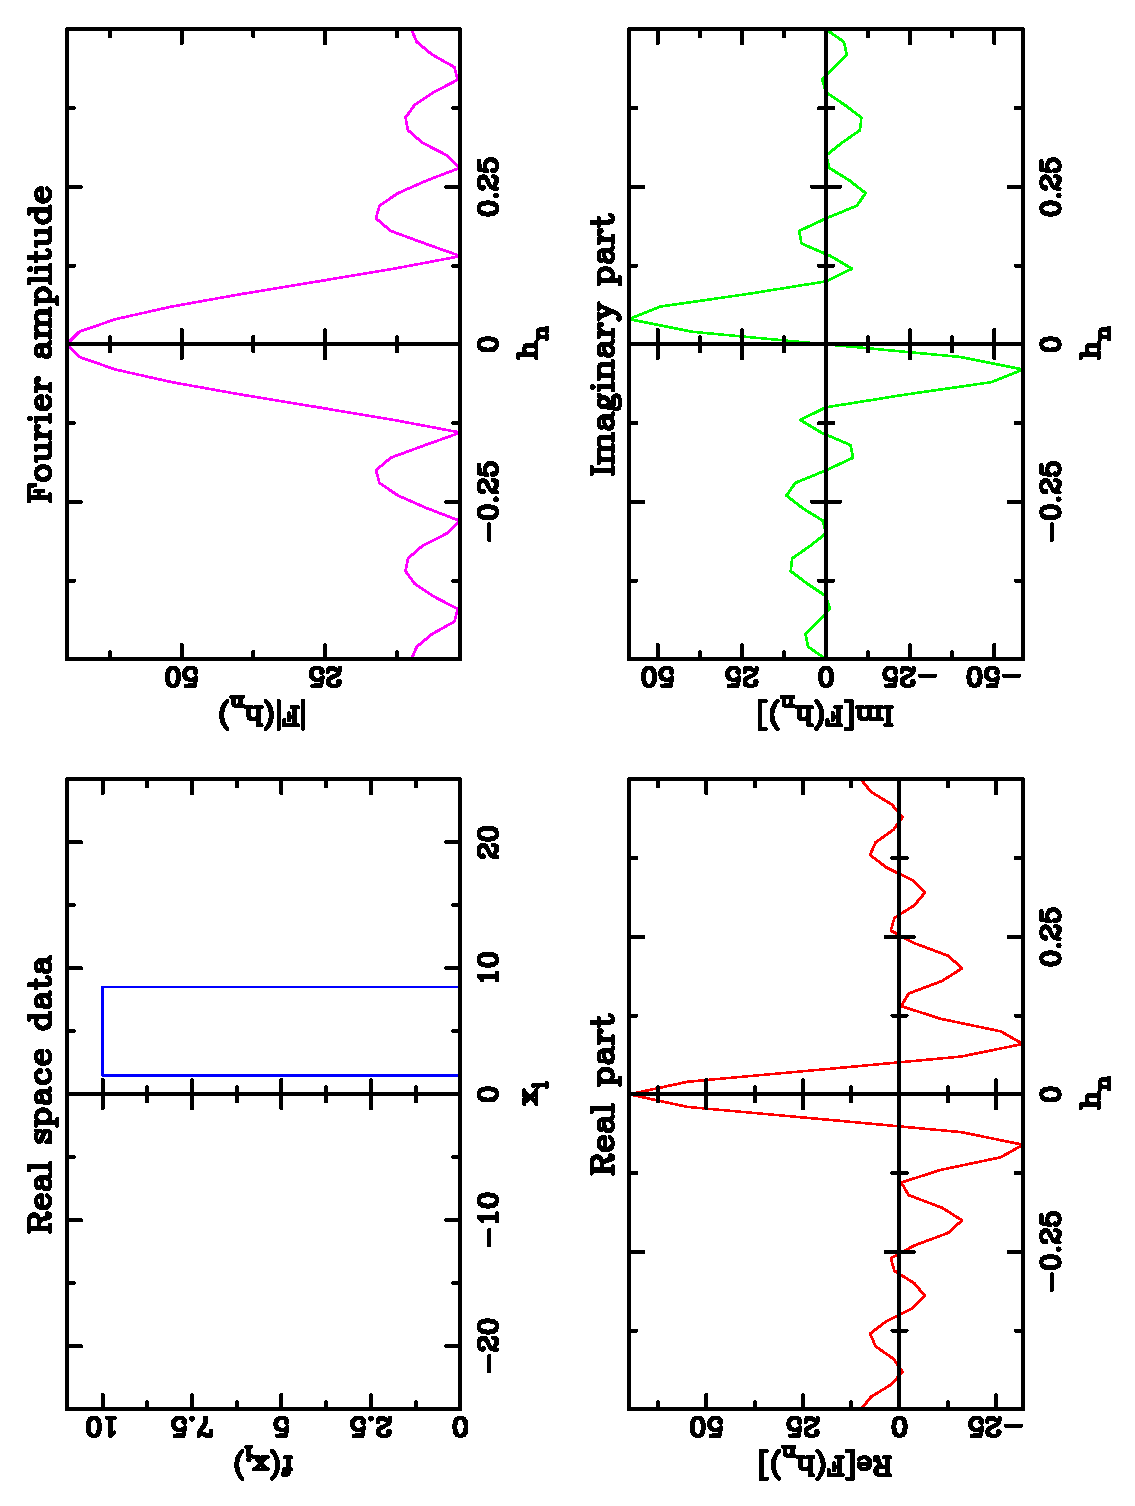
\includegraphics[scale=0.5, angle=270.0]{mat.4.eps}
   \caption{Fourier transform of box function}
   \label{mat-fig4}
\end{figure}

The Fourier transform is a complex quantity and {\it KUPLOT} allows one
to select the real and imaginary part and/or amplitude and phase angle
to be stored as new data sets. \par

Let us consider a simple example, a box function as displayed in the
upper left panel of Figure \ref{mat-fig4}. Our data set has $N=50$
points and a grid size of $\Delta x = 1.0$. Using equation \ref{mat-eq1}
we find the grid size in Fourier space to be $1/50 = 0.02$ and a
calculated range of $-1/2\Delta x = -0.5$ to $0.5$. In our example
the command for the calculation of the Fourier transform is:

\begin{MacVerbatim}
  four ria
\end{MacVerbatim}

The parameter {\tt ria} specifies that we want to keep the {\bf
r}eal and {\bf i}maginary part as well as the {\bf a}mplitude of the
Fourier transform. All three parts and the box function are shown in
Figure \ref{mat-fig4}.


%------------------------------------------------------------------------

\section{Other functions \label{mat-other}}

The command {\tt deriv ik,n} will calculate the numerical n-th
derivative of data set {\tt ik} and store the result a a new data
set. The convolution of two data sets can be calculated using the
command {\tt conv}. Both data sets need to have a common equidistant
set of $x$ values. 

%------------------------------------------------------------------------
% Chapter:  Fitting
%------------------------------------------------------------------------

\chapter{Least square fitting \label {fit}}

This chapter describes the least-square (LS) fitting segment of the
program {\it KUPLOT}. The user can choose between polynomial, Gaussian
and Lorentzian for 1D data or a Gaussian for 2D data. Furthermore
this version of {\it KUPLOT} supports user defined theory functions
thus allowing for virtually any fit function desired. A description
of the LS method itself is beyond the scope of this manual and the
reader might refer to various text books on statistics or numerical
mathematics. For a list of all fit related commands of {\it KUPLOT}
check the online help or the command reference manual.

%------------------------------------------------------------------------

\section{Fitting 1d data sets \label{fit-1d}}

Starting point for a LS refinement is a loaded data set ($x_{i}, y_{i}$),
the selection of a suitable theory function $y(x_{i},p)$ to describe
the data and a set of starting values for the fit parameters $p$.
The program {\it KUPLOT} offers the following three predefined theory
functions and additionally allows the use of a user defined function
(see section \ref{fit-user}).

\begin{eqnarray}
    y(x_{i},p) & = & \sum_{n=0}^{N} p_{n} x_{i}^{n}
    \label{fit-1d-eq1}  \\
    y(x_{i},p) & = & \sum_{n=0}^{N} p_{n} T_{n}(x_{i}) \\
               & with & T_{n}(x)=\cos(n \arccos x)
    \label{fit-1d-eq1b}\nonumber \\
    y(x_{i},p) & = & p_{1} + p_{2}x_{i} +
                     \sum_{n=1}^{N} p_{1,n}\cdot\exp\left\{
                     \frac {-(x_{i}-p_{2,n})^{2}}{\sigma_{n}^{2}}\right\}
    \label{fit-1d-eq2}  \\
    y(x_{i},p) & = & p_{1} + p_{2}x_{i} +
                     \sum_{n=1}^{N} p_{1,n}\cdot\left\{\frac{\sigma_{n}^{2}}
                     {(\sigma_{n}^{2}+4(x_{i}-p_{1,n}))^{2}}\right\}
    \label{fit-1d-eq3} \\
    & with & \sigma_{n} = \left\{ \begin{array}{ll}
                 p_{3,n} \cdot p_{4,n} & \mbox {for $x_{i} < p_{2,n}$}\\
                 \frac{p_{3,n}}{p_{4,n}} & \mbox {else} \\ \end{array}
                 \right.
    \nonumber
\end{eqnarray}

Let us have a closer look at these theory functions.  The first one
shown in equation \ref{fit-1d-eq1} is a simple polynomial of the
order of $N$ which can be defined by the user.  The fit parameters
$p_{n}$ are the corresponding coefficients.  Note that {\it KUPLOT}
actually numbers the fit parameters starting with one, i.e.
parameter one corresponds to the term $x^{0}$. Similarly equation
\ref{fit-1d-eq1b} defines a Chebyshev polynomial.
\par

The next function (equation \ref{fit-1d-eq2}) is a sum of $N$ Gaussians and
a linear background defined by the first two parameters $p_{1}$ and
$p_{2}$.  The number of Gaussians to be used is defined by the user.  Each
Gaussian is represented by a set of four fit parameters: $p_{1,n}$ is its
peak height and $p_{2,n}$ is its peak position.  The half width of the
Gaussian (as well as the Lorentzian) is defined by a half width parameter
$p_{3,n}$ and an asymmetry parameter $p_{4,n}$.  Obviously the symmetric
case is given by $p_{4,n} = 1.0$.  The Lorentzian theory function (equation
\ref{fit-1d-eq3}) is defined by a similar set of parameters.  Currently
both function types can not be used in combination except as user defined
theory function as described in section \ref{fit-user}.  \par


\begin{figure}[!tbhp]
   \centering
   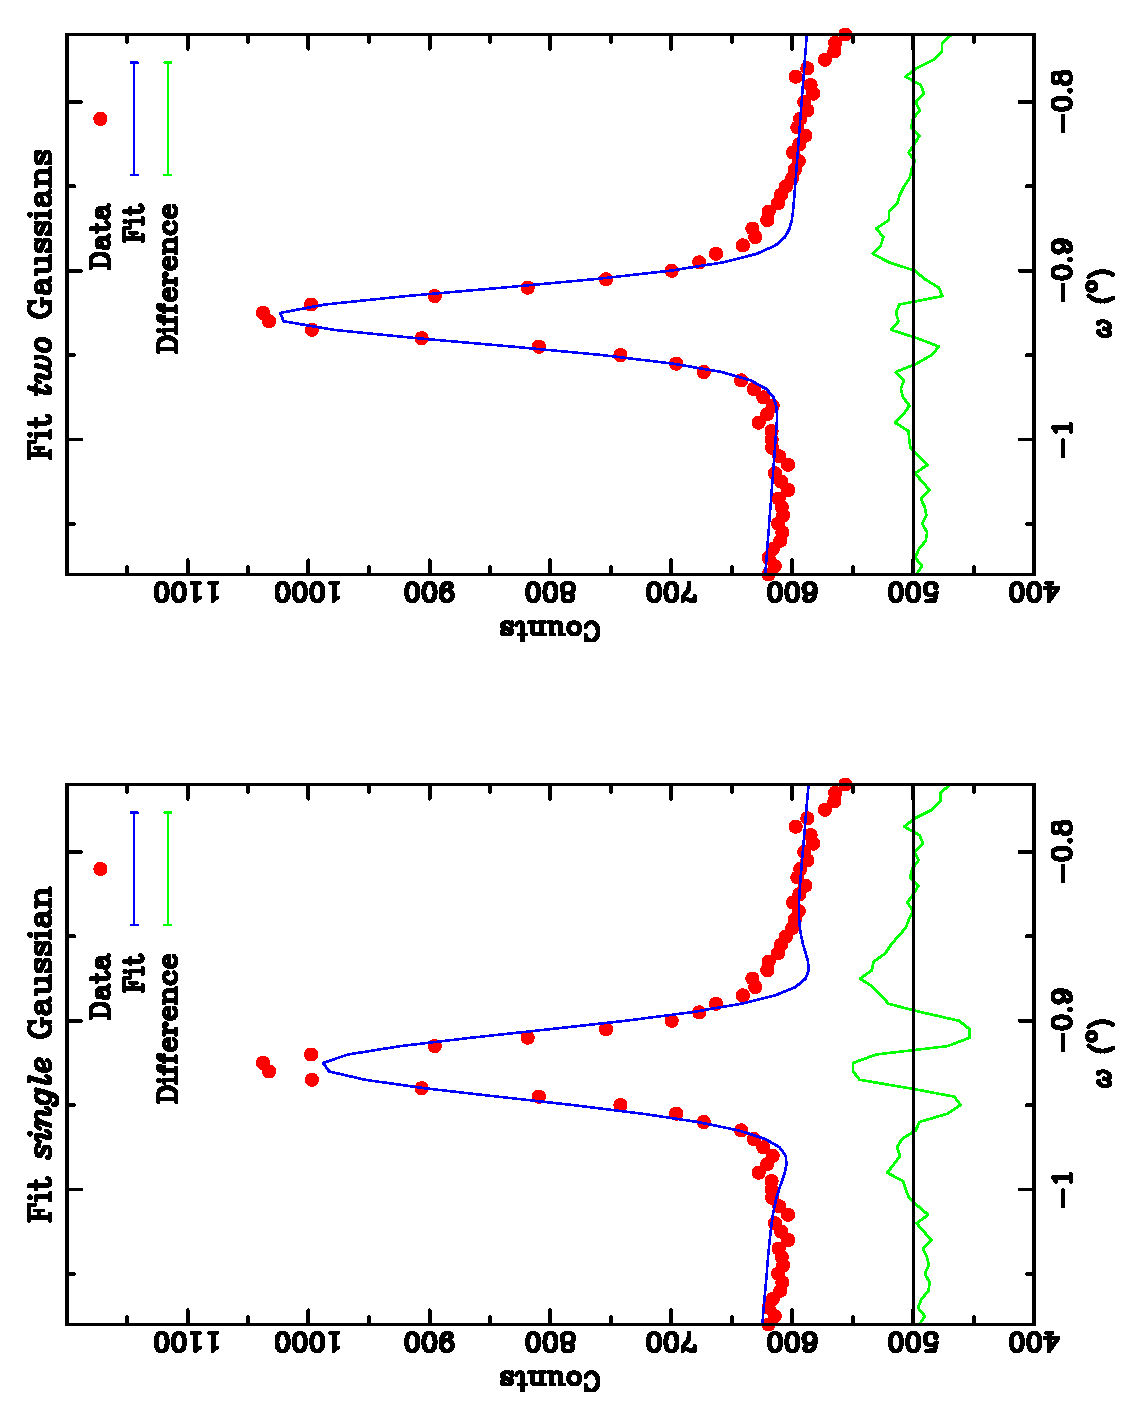
\includegraphics[scale=0.5, angle=270.0]{fit.1.eps}
   \caption{Fit results for 1D example}
   \label{fit-fig1}
\end{figure}

Now we will see the fitting segment of {\it KUPLOT} in action in the
following example.  The data set is the profile we have used in
examples before in Figure \ref{fra-fig1}. Assuming the corresponding
data are loaded as set one, the next step is to enter the LS
sub level of the program {\it KUPLOT}.  This is done by the command
{\tt fit} followed by the data set number that should be used as
observed data (line 1).  The macro is show below and as before the
line number are not part of the macro file itself.

\begin{MacVerbatim}
     1  fit 1
     2  #
     3  mfen 7
     4  func gaus,1
     5  par
     6  #
     7  run
     8  save
\end{MacVerbatim}

The command in line 3 sets the {\tt window} size used to determine
maxima within the plot which are used as defaults for the starting
values. The procedure is equivalent to the command {\tt smax}
explained in section \ref{mat-anal}. For our example the setting to
7 points will determine the main maximum correctly. Next (line 4)
the theory function is specified to be one Gaussian. Note that {\it
KUPLOT} determines the default starting values for the fitting
parameters $p$ at this stage and the command {\tt mfen} has to be
entered before to have an effect. Furthermore all current values of
the fit parameters, e.g. from a previous run, are replaced by the
new default values. The command {\tt par} (line 5) lists the current
parameter settings and after checking them on the screen we are
ready to go. The fit is started via the command {\tt run} in line 7
of our example command file. The fit progress is displayed on the
screen until the fits converges to a minimum or the maximum number
of cycles is reached. This maximum cycle number can be altered using
the {\tt cyc} command in the fitting sub level. In our example it
took 9 iterations to reach the minimum and the resulting parameters
are listed in table \ref{fit-tab1} on the left. Finally the results
are saved (line 8) as two data files containing the calculated and
difference data set and a text file summarizing the results.

\begin{table}[!t]
\centering
\begin{tabular}[b]{|l|c|c|c|}
  \hline
  {\bf Parameter} & {\bf One Gaussian} &
       \multicolumn{2}{|c|}{\bf Two Gaussians} \\
  \hline
            &     &      Gaussian 1 & Gaussian 2 \\
  \hline\hline
   Background $p_{1}$ &  506.(16)   & \multicolumn{2}{|c|}{  501.(10)} \\
   Background $p_{2}$ & -107.(18)   & \multicolumn{2}{|c|}{ -106.(11)} \\
  \hline
   Peak height        &  421.(9)    &  315.(10)  &   134.(10)   \\
   Peak position      & -0.9270(4) & -0.9277(3)  &  -0.9250$^{*}$ \\
   Half width         &  0.0374(9) &  0.0278(9)  &   0.0640$^{*}$ \\
  \hline
   R-value            &  2.1\%     &   \multicolumn{2}{|c|}{ 1.2\%} \\
  \hline
\end{tabular}
\caption{\label{fit-tab1}Results of example 1D fit}
\end{table}

The resulting plot of the observed and calculated data as well as
the difference between them is shown in Figure \ref{fit-fig1} again
on the left. Although there a reasonable agreement is achieved,
there are clearly visible differences especially at the tails of the
Gaussian. Note that we have fitted a symmetric Gaussian which is the
default, i.e. the parameter $p_{4,n}$ is set to 1.0 and not refined.
To refine this parameter use the command {\tt par 6,1}. The first
number is the number of the fit parameter (since we have two
background parameters it is 4+2=6) and the next number can be 1 for
refining or 0 for keeping the corresponding parameter fixed. An
optional third parameter allows one to alter the value of the fit
parameter. \par

To improve the fit we will try to fit two Gaussians located at the
same position to the data set. This will allow to model the sides of
the peak in a better way. The corresponding macro is shown below.
Lines 1--4 are the same as before except that we select two Gaussians
rather than one. Again we assume the profile is loaded as data set
one.

\begin{MacVerbatim}
     1  fit 1
     2  #
     3  mfen 7
     4  func gaus,2
     5  #
     6  par 7,1,0.0
     7  par 8,1,p[4]
     8  par 9,1,p[5]
     9  par10,0,p[6]
    10  par
    11  #
    12  run
    13  save
\end{MacVerbatim}
\normalsize

Since {\it KUPLOT} will only find one maximum a warning will be
displayed and we have to set the starting values for our second
Gaussian manually (lines 6--9). We set the peak height to 0.0 and
take the other parameters from the settings for the first Gaussian
using the variables {\tt p[i]}. Just to be sure we list the current
settings again (line 10) and the fit is started in line 12 by the
{\tt run} command. Finally the results are saved as before (line
13). The resulting parameters are listed in Table \ref{fit-tab1}. A
measure for the quality of a fit is the R-vale which is defined as:

\begin{equation}
    R=\sqrt{\frac{\sum\limits_{i=1}^{N} w_{i} (y_{i} - y(x_{i},p))^{2}}
                 {\sum\limits_{i=1}^{N} w_{i} y_{i}^{2}}}
    \label{fit-1d-eq-R}
\end{equation}

Here the sum goes over all $N$ data points ($x_{i},y_{i}$) and
$y(x_{i},p)$ is the theory function.  {\it KUPLOT} offers a variety
of weights $w_{i}$ to be selected to the fit.  The default we have
used in our example is $w_{i} = \frac{1}{y_{i}}$.  Check the online
help for the command {\tt wic} to obtain more information about
supported weighting schemes.  Inspection of the results for this
second fit shown in Table \ref{fit-tab1} and Figure \ref{fit-fig1}
clearly show that the second fit describes the data much better.
However the parameters marked with * in Table \ref{fit-tab1} could
not be refined and remained at their starting values.  Possible
steps to avoid that problem are to refine the parameters one by one
or change the setting of URF which controlled the {\it speed} of the
fit. A small value, e.g.  0.1, will converge quickly to the minimum
but in case of a more complex problem, the fit might fail.  A larger
value of URF on the other hand will change the parameters in each
iteration by a smaller amount and the fit might work.  However care
has to be taken to not end up in a local minimum.  The value of URF
(which stands for something very German - Unterer Relaxationsfaktor)
is altered via the command {\tt urf}.  The authors recommend playing
around with the various settings of the fit sub level to get familiar
with the least square fitting process.

%------------------------------------------------------------------------

\section{Fitting 2d data sets \label{fit-2d}}

Actually there is no principle difference between fitting a 2D or a 1D data
set.  The only theory function of 2D data currently available in {\it
KUPLOT} is a set of $N$ 2D Gaussians as defined in equation \ref{fit-2d-eq1}.
Each Gaussian is defined by eight parameters, peak height $p_{1,n}$, peak
position $p_{2,n}$ and $p_{3,n}$ in x- and y-direction, half widths
$p_{4,n}, p_{5,n}$ and asymmetry parameters $p_{7,n}, p_{8,n}$ for each
direction and a new parameter $p_{6,n}$ that defines the angle between the
main axes of the Gaussian and the coordinate system.  One additional
parameter describes a flat overall background.


\begin{eqnarray}
    z(x_{i},y_{i},p) & = & p_{1} +
                   \sum_{n=1}^{N} p_{1,n} \cdot
                   \exp\left\{\frac {r_{x}^{2}}{\sigma_{n}^{2}}\right\}
              \cdot\exp\left\{\frac {r_{y}^{2}}{\tau_{n}^{2}}  \right\}
    \label{fit-2d-eq1}\\
    \mbox {with\ }
         r_{x} & = & \cos(p_{6,n})(x_{i}-p_{2,n}) + \sin(y_{i}-p_{3,n})
    \nonumber \\
         r_{y} & = &-\sin(p_{6,n})(x_{i}-p_{2,n}) + \cos(y_{i}-p_{3,n})
    \nonumber \\
         \sigma_{n} & = & \left\{ \begin{array}{ll}
                  p_{4,n} \cdot p_{7,n} & \mbox {for $x_{i} < r_{x}$}\\
                \frac{p_{4,n}}{p_{7,n}} & \mbox {else} \\ \end{array}\right.
    \nonumber \\
         \tau_{n} & = & \left\{ \begin{array}{ll}
                  p_{5,n} \cdot p_{8,n} & \mbox {for $y_{i} < r_{y}$}\\
                \frac{p_{5,n}}{p_{8,n}} & \mbox {else} \\ \end{array}\right.
    \nonumber
\end{eqnarray}

This equation certainly looks more complex than the 1D equivalent and we
will illustrate the fitting of three 2D Gaussians to a section of the
diffuse scattering data used in the 2D examples before.  The data and the
fit result are shown in Figure \ref{fit-fig2}.  The observed data are shown
in the top view graph.  The maxima used to determine the starting values
for the fit are marked by black circles.  One of the major mistakes when
using the fit routine of {\it KUPLOT} are wrong starting values. The
calculated data are shown in the middle view graph using identical
contour line settings as for the data. The bottom view graph finally
shows the difference between observed and calculated data. The solid
black line is the zero level, red lines mark negative values and blue
lines stand for positive contour levels. Note that the contour line
interval used for the difference plot is only $\frac{1}{5}$ of the
interval used for the observed and calculated data in order to make
the differences more visible.

\begin{figure}[ptbh]
   \centering
   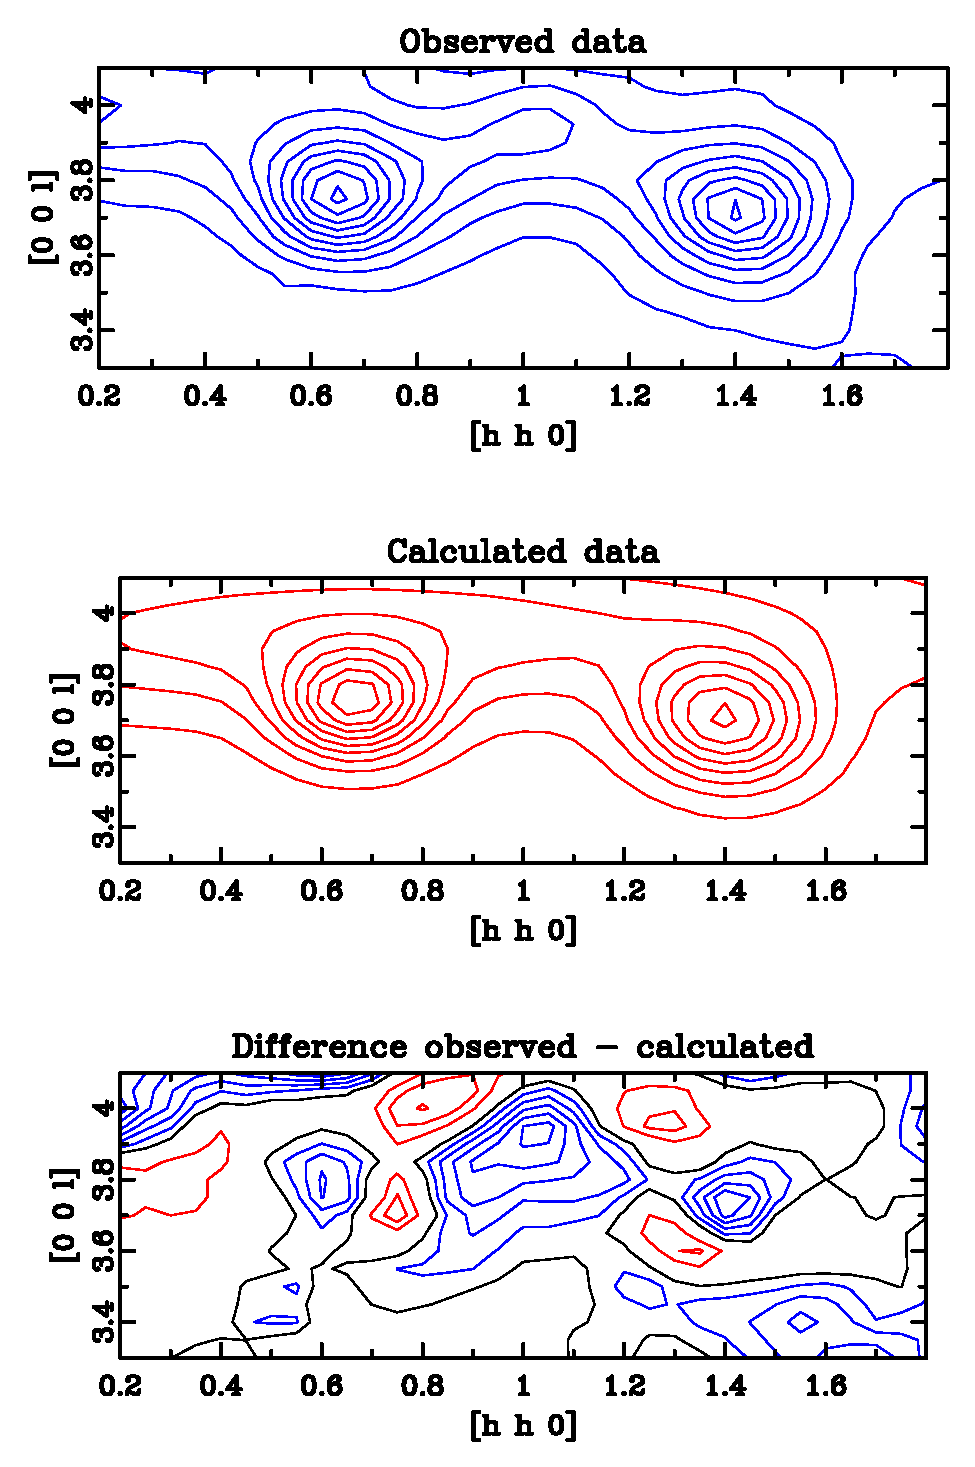
\includegraphics[scale=0.7, angle=0.0]{fit.2.eps}
   \caption{Fit results for 2D example}
   \label{fit-fig2}
\end{figure}

The macro file used for this example file is shown below. Again we
assume the observed data are already loaded as data set one.

\begin{MacVerbatim}
     1  fit 1
     2  #
     3  mfen 3
     4  func gau2,3
     5  par
     6  #
     7  run
     8  #
     9  par  7,1
    10  par 23,1
    11  #
    12  run
    13  save
    14  #
    15  exit
\end{MacVerbatim}

First we enter the fit sub level (line 1) to fit the theory function
to data set one. Before we select three 2D Gaussian theory functions
in line 4 we set the window size for determination for maxima used
as starting values to 3 data points. This will result in the three
maxima marked in Figure \ref{fit-fig2}. Line 5 displays the current
parameter settings for checking. Next (line 7) the fit is started.
As default the parameter $p_{6,n}$ determining the angle between the
principle axes of the Gaussian and the coordinate axes and the
asymmetry parameters $p_{7,n}$ and $p_{8,n}$ will be kept fixed.
After the first fit, the orientation of the Gaussian (parameter
$p_{6,n}$) for Gaussians one and three (the two strong peaks) are
refined as well (lines 9--12). Finally the data sets containing the
calculated data and the difference as well as the resulting
parameters are saved. When fitting interactively the command {\tt
plot} within the fit sublevel will plot the current fit on the
screen.
\par

Finally we want to have a look at the produced text file containing
the fit results (file extension {\it .erg}) for this example fit.
The line numbers are given for reference and as for the macro files
not part of the actual output file.  The first part contains general
information about the fit such as a title (lines 2--3), the used
theory function (line 4), the data file used (line 5), the number of
data points and parameters (lines 6--7).  Note that this is the
total number of parameters including those not actually refined.
Lines 8--10 show the current URF (see \ref{fit-1d}), the maximum
number of iterations, the setting for maxima determinations and the
used weighting scheme, in our case $w_{i} = \frac{1}{z_{i}}$.  The
next block of data in the output file show details of the fitting
process itself. Line 14 lists the value for $\sum (z_{i} -
z(x_{i},y_{i},p))^{2}$ for the last and the previous iteration step.
The difference between both is shown in the next line 15.  A big
difference normally indicates a {\it crashed} fit. The value of URF
changes during the refinement and the final value is shown in line
16.  If this value is not close to 1.0 at the end of the fit
something has gone wrong.  The next line shows the resulting R value
and the expected R value.  The ration of these values is also known
as the goodness-of-fit.  Finally all correlations between fitted
parameters that are greater than 0.8 are listed.  We are lucky
because our fit contains no highly correlated variables.

\begin{MacVerbatim}
     1   General fit parameter settings :
     2     Title            : KUPLOT 2D fit demonstration
     3                        January 1998
     4     Fit function     : Gaussian (2D)
     5     Data file name   : test.fit
     6     # of data pts.   :    561
     7     # of parameters  :     25
     8     Urf              :     .1000
     9     Max. cycle       :     30
    10     MFEN for maxima  :      3
    11     Weighting scheme : w(i) = 1.0/i
    12
    13   Information about the fit :
    14     Sum n-1    :  1038.98                 Sum n   :  1040.29
    15     Difference :  1.31653
    16     Urf final  :  1.00047
    17     R4 value   :  .106378                 R exp   :  .077327
    18
    19   Correlations larger than 0.8 :
    20     ** none **
    21
\end{MacVerbatim}

All remaining information of the output file are results of the
parameters used in the theory function.  In line 22 the number and
type of functions fitted are shown.  Next we have the result for the
overall background $p_{1}$ and its standard deviation (line 24). The
{\tt pinc} in the last column indicates whether the parameter was
refined (pinc = 1) or kept fixed to its starting value (pinc = 0).
The values for each parameter and the corresponding {\tt pinc} value
can be altered via the command {\tt par}.

\begin{MacVerbatim}
    22   Fitted  3 Gaussian(s) :
    23
    24     p( 1) : backgr. 1 :  69.2818     +-  .998061    pinc : 1.
    25
\end{MacVerbatim}

The rest of the output file contains three identical blocks with the
resulting parameters of the three Gaussians fitted to the observed data.
We show here just the results for Gaussian 1 (left maximum).

\begin{MacVerbatim}
    26   Gaussian :   1
    27
    28     p( 2) : peak      :  407.332     +-  11.3879    pinc : 1.
    29     p( 3) : position x:  .665616     +-  .002372    pinc : 1.
    30     p( 4) : position y:  3.74364     +-  .002798    pinc : 1.
    31     p( 5) : fwhm a    :  .237793     +-  .005545    pinc : 1.
    32     p( 6) : fwhm b    :  .235389     +-  .005938    pinc : 1.
    33     p( 7) : angle a,x : -98.8801     +-  85.1452    pinc : 1.
    34     p( 8) : asym. a   :  1.00000     +-  .000000    pinc : 0.
    35     p( 9) : asym. b   :  1.00000     +-  .000000    pinc : 0.
    36             integral  :  25.8344     +-  1.97653
\end{MacVerbatim}

Note that the asymmetry parameters were not refined, thus kept at the
default setting for a symmetric function.  The orientation for this
Gaussian (line 7) has a very large error which can be understood from the
resulting half width parameters (lines 31--32) which show a nearly isotropic
result.  Thus the definition of an orientation is quite arbitrary.  This
result is displayed here for demonstration purposes, normally the fit needs
to be repeated with a fixed orientation parameter for this Gaussian.  The
third Gaussian however (right maxima) has a significant orientation
parameter of $p_{6,n} = 33(8)^{\circ}$.  Finally (line 36) the integral for
each Gaussian with its standard deviation is given.

%------------------------------------------------------------------------

\section{User defined fit functions \label{fit-user}}

The final section of this chapter will demonstrate the use of an
arbitrary fit function. The fit process is not
different from the example described above, just the theory function is
entered as {\it KUPLOT} type of expression. Assuming your theory
function should be

\begin{equation}
    y(x_{i},p) = p_{1} \cdot \exp(- p_{2}x_{i}) \cdot \sin(x_{i}+p_{3}),
    \nonumber
\end{equation}

the corresponding command to define this theory function in the fit
sublevel of {\it KUPLOT} would look like this

\begin{MacVerbatim}
    func fx,3,p[1]*exp(-p[2]*r[0])*sin(r[0]+p[3])
\end{MacVerbatim}

The parameter {\tt fx} stands for a user defined function. The next
parameter is the number of fit parameters to be used for that
function. As last parameter, the function itself is given. The
variable r[0] stands for $x_{i}$ similar to the command {\tt func}
(see section \ref{mat-buildin}). The fit parameters are represented
by variables {\tt p[i]}. Since the nature of the fit function is
unknown, there is no calculation of default starting values. They
have to be supplied by the user via the command {\tt par}. Note that
{\it KUPLOT} is calculating the expression once after the {\tt func}
command is given to perform a syntax check. If no proper starting
values for {\tt p[i]} have been defined this calculation might fail,
e.g. by a division by zero. After the function is successfully
defined, the fit process proceeds as described in the previous
sections. The definition of a 2D theory function works exactly the
same way, use {\tt r[1]} for the values of $y_{i}$. The dimension of
the user defined theory function (1D or 2D) is given by the data set
used for the fit. \par

The derivatives needed for the least square refinement are
calculated numerically in contrast to the usage of analytical
derivatives used for the build in theory functions. In extreme cases
the calculation of these derivatives and subsequently the fit itself
might fail. In those cases it might be necessary to re-normalize the
observed values or to use a specialized fit package after all.

%------------------------------------------------------------------------


%------------------------------------------------------------------------
% Appendices
%------------------------------------------------------------------------

\appendix
\chapter{KUPLOT commands}
\section{Summary}
\par
Here is a list and brief description of valid KUPLOT commands. Further 
help can be obtained by typing the corresponding command name at the 
help prompt. 
\par
\begin{MacVerbatim}
News          : Information on program updates
achx/y/z      : Set labels for x, y and z-axis
alloc         : Allocate space for data set without loading one
angl          : Set angle between x- and y-axis
aver          : Set ratio between units on y and x-axis
branch        : Switch to discus, SUITE version only
buff          : Set reserved space outside of plotting frame
ccal          : Perform calculations with single data set
color         : Set pen colors
conv          : Calculate convolution of two data sets
costvalue     ! Set a value to be returned to DIFFEV
cmap          : Select color map
deriv         : Calculate the derivative
ecol          : Set color of error bars
etyp          : Set type of error bars
eval          : Evaluate expression
excl          : Exclude regions from 1D files
fill          : Set filling style
fit           : Enter least square fit sub level
fnam          : Toggle plot of filenames in upper left corner
font          : Set font size, type and color
fset          : Set type of plot frame (axis, tick marks, ..)
frames        : More information about the use of frames
func          : Create data set from given function
glat          : Smooth data set (sliding average)
grid          : Toggle plotting of a grid at main marker points
hart          : Set type for 2D plots (bitmap, contours, ..)
hcol          : Set color of contour lines
hlab          : Labeling of contour lines
hlin          : Set contour line parameters (also for bitmap)
hpak          : Set number of contour line packages
htyp          : Set line type for contour lines
iden          : Toggle plotting of user, data and time information
inte          : Integrate data set
ksav          : Save data set in various formats
kpara         : Plots parameters fitted with DIFFEV
kcal          : Perform calculations with two data sets (add, ..)
lart          : Set type for 1D plot (line, steps, spline)
lcol          : Set line color
load          : Read data set
ltyp          : Set line type
lwid          : Set line width
mark          : Set tick mark interval
match         : Calculate scale and offset to get best match bw. data
mcol          : Set marker color
mean          : Calculate average and stand. deviation for data set
merge         : Merge data sets (2D only)
mouse         : Activate the mouse
mtyp          : Set marker type
msiz          : Set marker size
nexus         : NeXus file support routines
orient        : Set paper orientation (landscape, portrait)
plot          : Display plot
prin          : Print plot
ptyp          : Set marker type for maxima
rdef          : Read KUPLOT settings from file
rebin         : Allows rebinning data to user defined grid
rese          : Reset
sann          : Set text annotations for plot
save          : Save plot as hardcopy
sdef          : Store KUPLOT settings on disk
show          : Show various settings
sleg          : Sets legend of plot
smax          : Determines maxima of data set
smooth        : Smooth data set (Savitzky-Golay algorithm)
sort          : Sort data set
spline        : Interpolate data set on grid given by different set
skal          : Set plot window
tit1/2        : Set plot titles
window        : Select graphics window
variables     : List of variables
errors        : List of error messages
\end{MacVerbatim}
\section{News}
\par
Here you can find updated info on the latest KUPLOT releases. 
\subsection*{2018\_Oct}
\par
Added the trend of the best value to the 'kpara' plot 
\subsection*{2018\_June}
\par
Revised the reaction to a CTRL-C 
\par
Added a ==$> $ 'set error, ... , "save" option 
\subsection*{2018\_May}
\par
Added the possibility to use a macro as fit 'function' 
\subsection*{2018\_Feb}
\par
Added a command 'kpara' to create a plot for DIFFEV 
\par
Added an optional parameter "partial" to the ==$> $ 'rvalue' command 
\par
Added optional parameters to the "load csv" command 
\subsection*{2018\_Jan}
\par
The new command 'costvalue' allows to set a global value 
for the cost funciton that is returned to DIFFEV. 
\par
The logical comparisons may now take the operators: 
$ <$, $ <$=, ==, /=, $> $=, $> $/ 
The classical fortran77 operators are still valid 
\par
New logical functions "isvar" and "isexp" can be used within an 
"if" construction. See help entry ==$> $'function' in the 
general "Command\_lang" section. 
\subsection*{2017\_Oct}
\par
The 'ni' format may now have a leading header that consists of 
lines that start with a '\#' in the first column 
\subsection*{2017\_Sep}
\par
Throughout the program the internal calculation of random numbers 
was changed to the FORTRAN 90 intrinsic function. 
\par
Added error messages for variable nx, ny, modified variable np to 
yield the total number of data points for 2D data sets as well. 
\subsection*{2017\_May}
\par
The 'save' command can now save graphics as a PDF file 
\subsection*{2017\_Jan}
\par
Added the option to read CSV files to 'load' command. 
\par
An unfortunate typing error in News/2016\_oct regarding the new 
refinement variable 
ref\_para[1...]   ( was misspelled as ref\_param[1...] ) 
is corrected in the  on-line help. 
\subsection*{2016\_Dec}
\par
At a few select points colors are introduced into the output. 
Currently these are just the error messages. 
\par
\subsection*{2016\_Oct}
\par
Global variables have been introduced that use the same syntax as 
user defined variables. This include just "pi" and variables related 
to the refinement. 
DIFFEV sets the value to these variables: 
ref\_generation  Current generation 
ref\_member      Current population size 
ref\_children    Current children size 
ref\_dimension   Number of parameters 
ref\_kid         Current child Updated for DISCUS and KUPLOT only 
ref\_indiv       Current individuum Updated for DISCUS and KUPLOT only 
ref\_para[1..]   Current trial parameters for current child 
\par
All colors can be referenced by their respective names as well as by 
their traditional numbers. See 'lcol', 'hcol', 'mcol' 'ecol' 
\par
All line types can be referenced by descriptive names as well as by 
their traditional numbers. See 'ltyp', 'htyp' 
\par
All marker types can be referenced by descriptive names as well as by 
their traditional numbers. See 'etyp', 'mtyp', 'ptyp' 
\subsection*{2016\_Feb}
\par
Minor upgrade, added a threshold function to ==$> $ 'ccal' 
\subsection*{2015\_Dec}
\par
Minor upgrade, increases the size of bitmaps KUPLOT can plot 
\subsection*{2015\_June}
\par
Starting with Version 5.1, we have migrated to a X-Window 
environment for WINDOWS as well. As a small side effect, 
the technique to jump to the desired folder has changed slightly. 
See the help entry on "cd" in the general "Command\_lang" section 
for further information. The process is described in the 
package manual as well. 
\section{achx/y/z}
{\bf achx $ \{$$ <$string$> $ $| $"OFF"$\} $ [, $ \{$"lin" $| $ "log"$\} $] \par }
{\bf achy $ \{$$ <$string$> $ $| $"OFF"$\} $ [, $ \{$"lin" $| $ "log"$\} $] \par }
{\bf achz $ \{$$ <$string$> $ $| $"OFF"$\} $ \par }
\par
\vspace{3pt}
This command sets the labels for the x- or y-axis. The label for 
the z-axis is only active when bitmaps are plotted and is used 
to label a wedge on the left side of the plot. As for the other 
axes the parameter "OFF" will turn off the plotting of the 
wedge which is the default. The optional parameter "lin" or 
"log" allows the user to toggle between a linear and logarithmic 
axis. 
\par
Because KUPLOT treats the ',' as a parameter separator it can not 
be used within the label $ <$string$> $. The command allows to build a 
label from a format text and variables/numbers. It is the same 
mechanism as described in -$> $ filenames. If the given parameter is 
"OFF", no label AND no numbers will be plotted at the corresponding 
axis. 
\par
Examples: 
\par
\begin{MacVerbatim}
achx 2 Theta       : will label x-axis with '2 Theta'
achy "PSD #%d",43  : will label y-axis with 'PSD #43'
\end{MacVerbatim}
\section{alloc}
{\bf alloc $ <$name$> $,$ <$len$> $ \par }
{\bf alloc $ <$name$> $,$ <$x$> $,$ <$y$> $ \par }
\par
\vspace{3pt}
This command allocates space for a new data set. This is e.g. required 
if a data set should be created using the FORTRAN interpreter of 
KUPLOT. The command 'alloc $ <$name,$ <$len$> $' allocated space for $ <$len$> $ 
points for a 2d data set. To allocate a 3d data sets, the size in x- 
and y-direction is given after the name of the data set. The parameter 
$ <$name$> $ just specifies a name for the data set (also used as default 
filename if the data set is saved). 
\section{angl}
{\bf angl [$ <$angle$> $] \par }
\par
\vspace{3pt}
This command allows to set the angle between the x- and y-axis for 
the currently active frame. Suitable angles are between 30 and 120 
degrees. If the command is entered without parameters, the value 
is set to 90.0 degrees. 
\section{aver}
{\bf aver [$ <$yx$> $] \par }
\par
\vspace{3pt}
This command sets the aspect ratio between the y- and the x-axis. 
A value of $ <$yx$> $=1.0 will force one unit on the x-axis to be as 
long as one unit on the y-axis. The value $ <$yx$> $ is the ratio 
y/x of the length of a unit of both axis. Is the parameter $ <$yx$> $ 
omitted, the plot will fill the complete drawing area. 
\section{bond}
{\bf bond \par }
{\bf bond $ <$ib$> $,$ <$dist$> $ [,$ <$sig$> $ [,$ <$it$> $,$ <$ic$> $,$ <$iw$> $]] \par }
\par
\vspace{3pt}
This command enables the plotting of lines between points that 
have a given distance, e.g. to include bonds in a crystal file 
plot. The first parameter $ <$ib$> $ is the number of the definition 
you are going to alter. The second parameter $ <$dist$> $ is the 
distance of points that shall be connected by a line. The distance 
is given relative to the current x-axis. To calculate the distances, 
the aspect ratio and the angle between the axes is used. Thus you 
will get the desired connection only for the correct aspect ratio 
(-$> $ aver) and angle between the axes (-$> $ angl). The other parameters 
are optional. The value $ <$sig$> $ sets the allowed relative deviation 
from the given distance, e.g. a value of 0.1 will allow distances 
of +- 10\% of the given value. The parameters $ <$ic$> $, $ <$it$> $ and $ <$iw$> $ 
set the line color, line type and line width of the connecting 
line, respectively (-$> $ lcol, ltyp, lwid). 
\par
In order to disable the plotting of a defined bond, just specify 
a zero distance, i.e. 'bond $ <$ic$> $,0.0'. 
\section{branch}
{\bf branch discus [, "-macro" $ <$macro\_name$> $ [ $ <$par1$> $ [ , $ <$par2$> $ ...]]] \par }
{\bf branch diffev [, "-macro" $ <$macro\_name$> $ [ $ <$par1$> $ [ , $ <$par2$> $ ...]]] \par }
\par
\vspace{3pt}
Active within the discus suite only! 
\par
Branches to the "discus" or "diffev" section. 
\par
Within this section any standard DISCUS command can be 
given. The behavior of "discus" is essentially the same 
as in the stand alone version. Likewise for DIFFEV. 
\par
The main use will branch to DISCUS while the discus section 
is run via run\_mpi from a DIFFEV slave. 
\par
Optionally the "-macro" qualifier instructs the suite to run the 
macro $ <$macro\_name$> $ (with its optional parameters) before the 
interactive session is started. 
\section{buff}
{\bf buff $ <$all$> $ \par }
{\bf buff $ <$left$> $,$ <$right$> $,$ <$bottom$> $,$ <$top$> $ \par }
\par
\vspace{3pt}
This command allows to alter the amount of drawing space KUPLOT 
reserves outside the plotting area for labels, titles etc.. The 
parameters given are relative to the size of the plot, e.g. a 
value of 0.3 will save 30\% of the width/height of the plot itself 
for axis numbers, labels etc. - note that if the reserved space 
is too small text might be wrapped around or cut off. 
\section{branch}
{\bf branch discus \par }
\par
\vspace{3pt}
Active within the discus suite only! 
\par
Branches to the "discus" section. 
\par
Within this section any standard DISCUS command can be 
given. The behavior of "discus" is essentially the same 
as in the stand alone version. 
\section{ccal}
{\bf ccal $ <$oper$> $,$ <$field$> $,$ <$ik$> $ [,$ <$value$> $] \par }
\par
\vspace{3pt}
This command allows data manipulation. All functions could also 
be performed using the FORTRAN type interpreter, but especially 
for large data sets this can be very slow. 
\par
The general syntax is the operation $ <$oper$> $ (see list below) that 
should be performed as first parameter followed by the field 
identifier $ <$field$> $ (see below), followed by the number of the 
data set $ <$ik$> $. Some operations require an additional parameter 
$ <$value$> $. 
\par
Here is a list of allowed operation parameters $ <$oper$> $: 
\par
\begin{MacVerbatim}
  "inv"  :  x -> 1/x         "squ"  :  x -> x**2
  "log"  :  x -> ln(x)       "add"  :  x -> x + <value>
  "exp"  :  x -> exp(x)      "mul"  :  x -> x * <value>
  "sqr"  :  x -> sqrt(x)     "abs"  :  x -> |a|
  "thr"  :  x < value -> -9999; value is thus a threshold,
\end{MacVerbatim}
 data below are considered invalid 
\par
The value "x" in the table above represents the coordinate selected 
by the $ <$field$> $ parameter. Allowed values are: 
\par
\begin{MacVerbatim}
  "wx" : x value of data set
  "dx" : standard deviation of x
  "wy" : y value of data set
  "dy" : standard deviation of y
  "wz" : z value of data set (for 3d data sets only)
\end{MacVerbatim}
\section{color}
{\bf color $ <$ic$> $,$ <$r$> $,$ <$g$> $,$ <$b$> $ \par }
\par
\vspace{3pt}
This command allows the user to change the color settings for 
the different pens. The parameter $ <$ic$> $ gives the pen number 
(0 for background) and $ <$r$> $,$ <$g$> $,$ <$b$> $ are the red, green and blue 
values to be uses ranging from 0.0 to 1.0. If no parameters are 
given, the current settings are displayed. 
\section{conv}
{\bf conv $ <$ik1$> $,$ <$ik2$> $ \par }
\par
\vspace{3pt}
This command calculates the convolution of data sets $ <$ik1$> $ and 
$ <$ik2$> $ and creates a new data set with the result. Both data sets 
must be on the same equidistant grid ! 
\section{cost}
{\bf costvalue  $ <$rvalue$> $ [, $ <$partial\_rvalue1$> $ ...] \par }
\par
\vspace{3pt}
Set a value that is to be retured to DIFFEV as the overall 
R-value. It will overwrite the current weighted R-value 
that was calculated with the ==$> $ 'rval' command. 
The value of $ <$rvalue$> $ can be any expression or real valued 
variable. This allows to calculate a combined, weighted 
R-value from several different calculations like single 
crystal, powder diffraction, PDF, etc. 
\par
If the partial R-values are provided as well, they will 
overwrite the corresponding partial R-values. 
\section{cmap}
{\bf cmap $ \{$ "gray" $| $ "fire" $| $ "kupl"  $\} $ \par }
{\bf cmap $ \{$ "read" $| $ "write"$\} $, $ <$fname$> $ \par }
{\bf cmap "invert" \par }
\par
\vspace{3pt}
This command allows to choose the color map to be used for printing 
bitmaps (see 'hart' command). The three build in color map are 
"gray", "fire" and "kupl" (the previous default color map). Color maps 
can also be read from a file using the command 'cmap read,$ <$fname$> $'. 
The format is of the form '\#RRGGBB' for each color map entry on a 
new line and 'RR', 'GG' and 'BB' are the 'red', 'green' and 'blue' 
values given in hexadecimal ranging from 00 to FF. The current 
color map can be saved to a file using the command 'cmap write,$ <$fname$> $'. 
Finally 'cmap invert' will simply invert the current color map. 
\par
The RGB values of the current color map can be shown using the 
command 'show color'. The color map entries can also be altered 
using the variable 'cmap [$ <$ic$> $,3]'. 
\section{deriv}
{\bf deriv $ <$ik$> $ [,$ <$order$> $] \par }
\par
\vspace{3pt}
This command calculates the $ <$order$> $th derivative of data set $ <$ik$> $. 
The result is stored as new data set. If $ <$order$> $ is omitted, the 
first derivative is calculated. 
\section{dsav}
{\bf dsav "gsas",$ <$file$> $ [,$ <$iname$> $] \par }
{\bf dsav "xml",$ <$file$> $ [,$ <$dtd-path$> $] \par }
{\bf dsav "merge",$ <$file$> $ \par }
\par
\vspace{3pt}
The parameter "gsas"  allows one to save all loaded data sets 
in GSAS file format. NOTE THAT THE CURRENT IMPLEMENTATION ASSUMES 
A LUJAN STYLE GSAS FILE. 
\par
The parameter "xml" will save the plot on PlotML (xml) format 
for viewing with 'plplot'. Currently only 1D data are supported. 
The optional second parameter allows one to specify the location 
of the DTD file needed to render the XML file. 
\par
The parameter "merge" will save a xyz-type file from all the 
loaded data sets with the following condition x=x, y=data set 
number and z=y. This can then be loaded using load zz, .. 
\section{ecol}
{\bf ecol $ <$ik$> $,$ <$c$> $ \par }
\par
\vspace{3pt}
This command sets the error bar color for the data set $ <$ik$> $. 
The colors are numbered like the pens on a HP7475 plotter. Allowed 
values for $ <$c$> $ are listed in the table, Alternatively you can use 
the color name (without blanks i.e. darkblue etc.) 
\par
The allowed default color values $ <$icol$> $ are listed below. Note 
that they can be changed by the user via the command 'color'. 
\par
\begin{MacVerbatim}
  1 : red       5 : yellow        9 : dark blue      13 : cyan
  2 : green     6 : black        10 : dark magenta   14 : dark cyan
  3 : blue      7 : dark red     11 : dark yellow    15 : white (!)
  4 : magenta   8 : dark green   12 : gray
\end{MacVerbatim}
\section{etyp}
{\bf etyp $ <$ik$> $,$ <$p$> $ \par }
\par
\vspace{3pt}
This command sets the type of error bars to be use for the data 
set number $ <$ik$> $. Allowed values for $ <$p$> $ are: 
\par
\begin{MacVerbatim}
  0 : {"noerror"|"none"} : no error bars are drawn
  1 :  "xbar"            : only error bars in x-direction
  2 :  "ybar"            : only error bars in y-direction
  3 :  "cross"           : error bars in both directions
\end{MacVerbatim}
\section{excl}
{\bf excl $ <$ik$> $,$ <$left$> $,$ <$right$> $ \par }
\par
\vspace{3pt}
This command allows the user to exclude the area between $ <$left$> $ 
and $ <$right$> $ from data set $ <$ik$> $. The values within the range 
are replaced by the linear interpolation between $ <$left$> $ and 
$ <$right$> $, i.e. the closest data points to the specified values. 
If $ <$left$> $ is outside the data range, all points up to $ <$right$> $ 
are removed. If $ <$right$> $ is outside the data range, all points 
from $ <$left$> $ onwards are removed. 
\section{fill}
{\bf fill $ <$ik$> $,$ <$fc$> $,$ <$ft$> $ [,$ <$xmin$> $,$ <$xmax$> $] [,$ <$ymin$> $,$ <$ymax$> $] \par }
\par
\vspace{3pt}
This command sets the filling style for data set $ <$ik$> $. The data 
set is treated as a polygon and is filled between the data and 
the baseline. The fill color is defined by $ <$fc$> $ (see lcol for 
color definitions). The following fill types $ <$ft$> $ are currently 
supported: 
\par
\begin{MacVerbatim}
  1: "solid"     : solid fill    5: "bsolid" : type 1 plus border
  2: "slash"     : hashed (/)    6: "bslash" : type 2 plus border
  3: "backslash" : hashed (\)    7: "bback"  : type 3 plus border
  4: "cross"     : cross hashed  8: "bcross" : type 4 plus border
\end{MacVerbatim}
The filled area is defined by the data points and a baseline, 
by default the connection between the end points of the current 
plotting area. However, the area to be filled can be limited 
using the optional parameters $ <$xmin$> $, $ <$xmax$> $ and $ <$ymin$> $, $ <$ymax$> $. 
\section{fit}
{\bf fit $ <$ik$> $ \par }
\par
\vspace{3pt}
This command enters the fit sub level and data set $ <$ik$> $ is taken 
as target data set. For an easy start, select a fit function 
with 'func' and start the fit using the 'run' command. The result 
can be displayed with 'plot' and saved with 'save'. For more 
detailed information see the list of commands below: 
\par
\subsection*{commands}
{\bf Valid commands in this sub level are: \par }
\par
\begin{MacVerbatim}
@      : Executes a macro (see general help)
=      : Algebra (see general help)
cycle  : Sets maximum number of fit cycles
echo   : Echoes a string on the screen (see general help)
eval   : Evaluates an expression  (see general help)
exit   : Exits fit sub level
func   : Sets fit function
help   : Gives on-line help for 'fit' sub level (see general help)
macro  : Writes current fit parameters to a macro file
mark   : Sets interval for tick marks
mfen   : Sets parameter for maxima determination (fit start values)
output : Toggles fit screen output on/off
para   : Sets/modifies fit parameters
plot   : Plot results
range  : Sets data range used for refinement
run    : Start the fit
save   : Save fit results
show   : Show settings and fit results
skal   : Sets region for plotting window (see general help)
system : Executes operating system command (see general help)
urf    : Sets urf value
wait   : Waits for user input (see general help)
wic    : Sets weighting scheme
\end{MacVerbatim}
\subsection*{cycle}
{\bf cycle $ <$n$> $ \par }
\par
\vspace{3pt}
This command sets the maximum number of cycles to $ <$n$> $. If a minimum 
is found in less cycles, the fit will stop before $ <$n$> $ cycles are 
finished. 
\subsection*{func}
\par
This command allows to set the fit function. After this command is 
called, KUPLOT will calculate starting values and destroy possible 
previous fit results, which should be saved ('save') before this 
command is called. The starting values for some functions use the 
'smax' function. You can set the window size using the 'mfen' command. 
See also -$> $ 'smax'. The following table shows the currently allowed 
functions: 
\par
\begin{MacVerbatim}
function   2d   3d   what            <par>
-----------------------------------------------------------
 "poly"    yes  no   polynomial         order of the polynomial
 "cheb"    yes  no   Chebyshev poly. order of the polynomial
 "gaus"    yes  yes  Gaussian        number of Gaussians
 "lore"    yes  no   Lorentzian      number of Lorentzians
 "pseudo"  yes  no   Pseudo-Voigt    number of Pseudo-Voigts
 "fx"      yes  yes  User defined    # parameters and function
 "ma"      yes  yes  User macro      # parameters and macro name
 "back"    yes  no   Background      # of background parameters
 "gsas"    yes  no   TOF profile     see text
\end{MacVerbatim}
Select a fit function from the list below for more information: 
\subsubsection{poly}
{\bf func "poly" [,$ <$par$> $] \par }
\par
\vspace{3pt}
A polynomial function p[1] + p[2]*r[0] + p[3]*r[0]**2 + ... 
is used. The parameter is the order of the polynomial. 
\subsubsection{gaus}
{\bf func "gaus" [,$ <$par$> $] \par }
\par
\vspace{3pt}
The fit uses $ <$par$> $ Gaussian functions. Two parameters (no. 1 
and 2) are refined for the background and each Gaussian peak used 
four parameters: 
\par
\begin{MacVerbatim}
p[3] Peak height
p[4] Position
p[5] FWHM
p[6] Asymmetry
\end{MacVerbatim}
A Gaussian function with linear background is used as: 
p[1] + p[2]*r[0] + p[3]*exp(-4*ln(2)*(r[0]-p[4])**2/p[5]**2) 
Note that the peak height rather than the integral intensity 
is refined. 
\subsubsection{lore}
{\bf func "lore" [,$ <$par$> $] \par }
\par
\vspace{3pt}
The fit uses $ <$par$> $ Lorentzian functions. Two parameters (no. 1 and 2) 
are refined for the background and each Lorentzian peak used four 
parameters: 
\par
\begin{MacVerbatim}
p[3] Peak height
p[4] Position
p[5] FWHM
p[6] Asymmetry
\end{MacVerbatim}
A Lorentzian function with linear background is used: 
p[1] + p[2]*r[0] + p[3]*p[5]**2/(p[5]**2 + 4*(r[0]-p[4])**2) 
Note that the peak height rather than the integral intensity 
is refined. 
\subsubsection{pseudo}
{\bf func "pseudo" [,$ <$par$> $ [,$ <$origin$> $ [,$ <$n\_backgrd$> $ ]] \par }
\par
\vspace{3pt}
The fit uses $ <$par$> $ Pseudo-Voigt functions. $ <$n\_backgrd$> $ parameters 
(no. 1, .. to $ <$n\_backgrd$> $) are refined for the background and each 
Pseudo-Voigt peak used six parameters: 
\par
\begin{MacVerbatim}
p[3] eta
p[4] integral intensity
p[5] Position
p[6] FWHM
p[7] Asymmetry parameter 1
p[8] Asymmetry parameter 2
\end{MacVerbatim}
The Pseudo-Voigt function is used in the form: 
\par
\begin{MacVerbatim}
background + Intensity*(eta*L + (1-eta)G)*Asymmetry
\end{MacVerbatim}
with Lorentzian part as: 
\begin{MacVerbatim}
L = 2/pi*FWHM / ( FWHM**2 + 4*(x-POSITION)**2 )
\end{MacVerbatim}
and Gaussian part as: 
\begin{MacVerbatim}
G = 2*sqrt(ln(2)/pi)/FWHM * exp ( -4ln(2) * (x-POSITION)**2/FWHM**2 )
\end{MacVerbatim}
The asymmetry function is defined as: 
\par
\begin{MacVerbatim}
ASYMMETRY = 1 + (p[7]*FA(z) + p[8]*FB(z))/ tan(POSTION)
FA(z) = 2*z*exp(-z**2)
FB(z) = 2*(2*z**2-3)*FA(z)
z = (x-POSITION)/FWHM
\end{MacVerbatim}
The background is calculated as a polynomial of order 
(n\_backgrd-1): 
\par
\begin{MacVerbatim}
p[1] + p[2]*(x-origin) + p[3]*(x-origin)**2 + ...
or more exactly:
SUM p[i]*(x-origin)**(i-1)
\end{MacVerbatim}
where origin is the third optional parameter from the command 
line. If this parameter is omitted, the origin is set to zero. 
To describe a locally bent background, one should set the 
origin of the background to a position within the refined 
x-range instead of zero. The value of the origin is not refined. 
\par
The last optional parameter defines the number of background 
parameters to be used. If it is omitted, the number of 
background parameters is set to 2. 
\subsubsection{fx}
{\bf func "fx",$ <$ip$> $,$ <$function$> $ \par }
\vspace{3pt}
KUPLOT allows the user to fit a user defined function to a given 
1D as well as 2D data set. The first parameter after "fx" specifies 
the number of parameters. Refer to the parameters in the expression 
for the function as p[1],p[2],.... The x-variable is r[0] and the 
y-variable (for 2D data sets) is r[1]. Note, that possible values 
stored in these variables are lost. It sounds complicated, but the 
following examples should help: 
\par
\begin{MacVerbatim}
func fx,3,p[1]+p[2]*exp(p[3]*r[0])   : Fit a+b*exp(c*x)
func fx,2,p[1]*r[0]+p[2]*r[1]        : Fit a*x + b*y (2D data set)
\end{MacVerbatim}
For a syntax check, the expression is calculated once after entering 
this command. If the parameter values p[i] are not set to proper 
start values, a error might occur, i.e. division by zero. 
\subsubsection{ma}
{\bf func "ma",$ <$ip$> $,$ <$macro\_name$> $ \par }
\vspace{3pt}
KUPLOT allows the user to fit a user defined function inside a 
macro to a given 1D as well as 2D data set. The first parameter 
after "fx" specifies the number of parameters. Refer to the 
parameters in the expression for the function as p[1],p[2],.... 
The x-variable is r[0] and the y-variable (for 2D data sets) 
is r[1]. Note, that possible values stored in these variables 
are lost. 
\par
The macro can use expressions, loops and if constructions, 
nested macros are allowed as well. 
For a full use of the discus\_suite, use a combination of a 
'top' and 'quit' command. With the 'top' command the macro 
steps to the top level at the discus\_suite. From there on 
all commands can be used. 
\par
The final function value must be given on a 'value' command, 
the derivatives on a 'deriv' command. For these command you 
must have left the 'top' section via a 'quit'. 
As simple macro would be: 
value p[1]*r[0]                  ! Fit a*x 
deriv 1, r[0]                    ! derivative with respect to p[1] 
finished 
\par
or absolutely eqivalently: 
r[100] = p[1]*r[0] 
value r[100]                     ! Fit a*x 
deriv 1, r[0]                    ! derivative with respect to p[1] 
finished 
\par
More involved, create a structure, calculate bond length as the 
function value: 
\par
r[101] = p[1]                    ! Copy KUPLOT variables to global 
r[102] = p[2] 
top                              ! Go to top level menu 
  discus 
    read 
      free 
    insert C, r[101], 0,0, 0.1 
    insert C, r[102], 0,0, 0.1 
    r[200] = x[1]-x[2]           ! the function value 
    r[201] =  1.0                ! the derivative with respect to p[1] 
    r[202] = -1.0                ! the derivative with respect to p[2] 
  exit 
quit                             ! Quit the top level menu back to fit 
value r[200] 
deriv 1, r[201] 
deriv 2, r[202] 
finished 
\par
It sounds complicated, but the following examples should help: 
\par
\begin{MacVerbatim}
func ma,3, one.mac                   : Fit a+b*exp(c*x)
\end{MacVerbatim}
Inside macro "one.mac" use the lines: 
value p[1]+p[2]*exp(p[3]*r[0])   ! Fit a+b*exp(c*x) 
deriv 1, 0.0                     ! derivative with respect to p[1] 
deriv 2, exp(p[3]*r[0])          ! derivative with respect to p[2] 
deriv 3, p[2]*exp(p[3]*r[0])*r[0]! derivative with respect to p[3] 
finished 
\par
The last command 'finished' is required inside these macros to 
return to the fit routine. 
\par
\begin{MacVerbatim}
func ma,2, two.mac                   : Fit a*x + b*y (2D data set)
\end{MacVerbatim}
Inside macro "two.mac" use the lines: 
value p[1]*r[0]+p[2]*r[1]        ! Fit a*x + b*y 
deriv 1, r[0]                    ! derivative with respect to p[1] 
deriv 2, r[1]                    ! derivative with respect to p[2] 
finished 
\par
\begin{MacVerbatim}
func ma, 2
\end{MacVerbatim}
For a syntax check, the expression is calculated once after entering 
this command. If the parameter values p[i] are not set to proper 
start values, a error might occur, i.e. division by zero. 
\subsubsection{gsas}
{\bf func "gsas",$ <$ptype$> $,$ <$bank$> $,$ <$iparm-file$> $ \par }
\par
\vspace{3pt}
KUPLOT allows the refinement of a GSAS profile function for TOF 
data. For details about the parameters and definitions of these 
functions, please refer to the GSAS manual. The parameters are 
$ <$ptype$> $ to select the profile function type, $ <$bank$> $ to select 
the bank number and $ <$iparm-file specifies the GSAS style 
instrument parameter file. The starting values are read from this 
file. Please also note, that the x-values are expected to be TOF. 
\subsubsection{back}
{\bf func "back",$ <$icalc$> $ [,$ <$par$> $] \par }
\vspace{3pt}
The fitting of a background is calculated as: 
\par
\begin{MacVerbatim}
y(dataset) = scale*y(dataset icalc) + SUM xx**parameter
\end{MacVerbatim}
Thus KUPLOT takes the data set $ <$icalc$> $ as input values, which are 
scaled and to which a polynomial function is added. This sum is 
fitted to the current dataset which was selected by the 'fit' command. 
\par
The scale parameter is p[1], all higher parameters act as exponents 
to the background polynomial. Thus p[2] is a constant background, 
p[3] a linear background etc. The xx argument of the polynomial 
is calculated as (x - xmin), where x is the x-value of each given 
data point and xmin the minimum x-value. Thus, the values of the 
background polynomial change if you fit to a changed x-range! 
\par
\begin{MacVerbatim}
<par>  effect
1      scale factor only
2      scale factor + constant background
3      scale factor + constant + linear background
N      scale factor + background polynomial of oder (N-2)
\end{MacVerbatim}
\subsection*{help}
{\bf help $ <$command$> $ \par }
\par
\vspace{3pt}
Displays this help text, for help for a certain command type help 
command. See help entry on main level for more details. 
\subsection*{macro}
{\bf macro $ <$filename$> $ \par }
\par
\vspace{3pt}
This command saves the current parameters in a KUPLOT macro file. 
This allows to set the parameter values in a later session using 
@$ <$filename$> $ from the FIT sub level. 
\subsection*{mfen}
{\bf mfen $ <$if$> $ \par }
\par
\vspace{3pt}
This command sets the 'window size' for maxima determination used 
to compute starting values for functions GAUS and LORE. For details 
about the $ <$if$> $ value see command -$> $ smax. 
\subsection*{output}
{\bf output $ \{$ "on" $| $ "off" $\} $ \par }
\par
\vspace{3pt}
This command allows to specify if the progress of the fit should be 
displayed on the screen ("on") or not ("off"). 
\subsection*{para}
{\bf para \par }
{\bf para $ <$ip$> $,$ <$pinc$> $ [,$ <$value$> $] \par }
{\bf para $ \{$ "save" $| $ "load" $\} $ \par }
\par
\vspace{3pt}
This command allows to modify the fit parameters. If the command 
is called alone, the current parameters are displayed. A single 
parameter $ <$ip$> $ can be set to a value $ <$value$> $. The value $ <$pinc$> $ 
specifies if the parameter should be refined ($ <$pinc$> $ = 1) of should 
be kept fixed ($ <$pinc$> $ = 0). If $ <$value$> $ is omitted the current value 
will be used. 
\par
A set of parameters can be internally stored ('para save') and loaded 
later back in the parameter array ('para load'). Each save command 
will overwrite previously stored values. 
\subsection*{plot}
{\bf plot \par }
\par
\vspace{3pt}
This command displays the current fit result with the current plot 
settings (like the plot command in the main level). 
\subsection*{range}
{\bf range $ \{$"all" $| $ "plot"$\} $ \par }
\par
\vspace{3pt}
This command allows one to select which part of the data are used 
for the refinement. If set to "all", all data are used. If set to 
"plot" only the data shown on the current plot window are used. 
This is useful if one wants to refine e.g. just a single Gaussian 
in a data set without having to manipulate the data set itself. 
\subsection*{run}
{\bf run \par }
\par
\vspace{3pt}
This command starts the fit. 
\subsection*{save}
{\bf save \par }
\par
\vspace{3pt}
This command saves the current fit results. The output filename 
is the filename of the input data set with the following extensions: 
\par
\begin{MacVerbatim}
  .erg  : text file with fit results
  .fit  : calculated data set
  .dif  : difference between observed and calculated data set
\end{MacVerbatim}
\subsection*{show}
{\bf show [ $ \{$ "general" $| $ "fit" $| $ "para" $\} $ ] \par }
\par
\vspace{3pt}
This command shows fit settings and results. If the command is called 
without parameters, all information is printed on the screen. The 
command 'show general' will display only general fit settings, 'show 
fit' the fit results like R values and 'show para' will list the 
resulting parameters. 
\subsection*{urf}
{\bf urf $ <$u$> $ \par }
\par
\vspace{3pt}
This command sets the URF (some German: Unterer Relaxations Faktor) 
for the fit. This value determines who 'fast' the fit will move to 
its minimum or how much the parameter values are changed in each 
cycle depending on the deviations. A small value (e.g. 0.1) might 
lead to a fast convergence but might also miss the minimum. A larger 
value (e.g. 100.0) will give a slow convergence which more certain 
finds the minimum, but might be caught in local minima rather than in 
the global one. 
\par
Understood ? Well just try different values until your fit converges 
nicely to the global minimum. 
\subsection*{wic}
{\bf wic $ <$w$> $ [,$ <$K$> $] \par }
\par
\vspace{3pt}
This command defines the weighting scheme to be used for the fit. The 
valid values for $ <$w$> $ are: 
\par
\begin{MacVerbatim}
  "one"  : w(y) = 1.0              "sqa"  : w(y) = y**2
  "sqrt" : w(y) = SQRT(y)          "inv"  : w(y) = 1/y
  "log"  : w(y) = LOG(y)           "isq"  : w(y) = 1/SQRT(y)
  "lin"  : w(y) = y                "dat"  : w(y) = 1/DY (error data set)
  "bck"  : w(y) = exp(-K*(y-ycalc))
\end{MacVerbatim}
The second parameter is only needed for the weighting scheme "bck". 
\section{fnam}
{\bf fnam [ $ \{$"on" $| $ "off"$\} $ ] \par }
\par
\vspace{3pt}
This command determines weather the filename should be plotted for 
every data set in the upper right corner. Called without parameters, 
filename plotting is switched off. 
\section{font}
{\bf font $ <$prop$> $,$ <$value$> $,.. \par }
\par
\vspace{3pt}
This command allows to set font attributes for the active frame. 
The settings can be displayed by entering the command 'font' 
without parameters or using the command 'show font'. For a list 
of escape sequences and special characters see entry PGPLOT below. 
The available font properties $ <$prop$> $ are listed below: 
\par
\subsection*{PGPLOT}
{\bf Special characters \par }
\par
\vspace{3pt}
The use of the PGPLOT library allows KUPLOT users to use a variety 
of escape sequences and special characters in all text related 
functions of KUPLOT. 
\par
\begin{MacVerbatim}
\u  : start superscript, or end subscript
\d  : start sub, or end superscript (e.g. cm\u-2\d)
\b  : backspace (draw next character on top of current one)
\fn : switch to normal font (1)
\fr : switch to roman font  (2)
\fi : switch to italic font (3)
\fs : switch to script font (4)

\\  : backslash              \x  : Multiplication sign
\.  : centered dot           \A  : Angstroem

\gx      : Greek character 'x' (e.g. \ga gives alpha, \gb beta, ..)
\(nnnn)  : character (nnnn) from the Hershey character set
\end{MacVerbatim}
\subsection*{color}
{\bf font "color",$ <$id$> $,$ <$icol$> $ \par }
\par
\vspace{3pt}
This command allows to alter the color of the font used to label the 
graph. The default is black for all fonts. The different types of 
text given by their $ <$id$> $ parameter are listed below: 
\par
\begin{MacVerbatim}
  1 : main title line               2: subtitle line
  3 : axis labels                   4: numbers at axis
  5 : text in text frame            6: filename & caption
\end{MacVerbatim}
The allowed default color values $ <$icol$> $ are listed below. Note 
that they can be changed by the user via the command 'color'. 
Alternatively you can use 
the color name (without blanks i.e. darkblue etc.) 
\par
\begin{MacVerbatim}
  1 : red       5 : yellow        9 : dark blue      13 : cyan
  2 : green     6 : black        10 : dark magenta   14 : dark cyan
  3 : blue      7 : dark red     11 : dark yellow    15 : white (!)
  4 : magenta   8 : dark green   12 : gray
\end{MacVerbatim}
\subsection*{just}
font "just", $ \{$ "left" $| $ "center" $\} $ 
\par
This command sets the text justification for the two title lines and 
the text within a text frame. 
\subsection*{size}
{\bf font "size",$ <$id$> $,$ <$size$> $ \par }
{\bf font "size",$ <$scale$> $ \par }
\par
\vspace{3pt}
This command sets the font size for text type $ <$id$> $ to $ <$size$> $ points. 
If a specified font size is not available, a fixed font will be used 
instead. The allowed $ <$id$> $ parameters are: 
\par
\begin{MacVerbatim}
  1 : main title line               2: subtitle line
  3 : axis labels                   4: numbers at axis
  5 : text in text frame            6: filename & caption
\end{MacVerbatim}
Alternatively if only one parameter is given after "size", all fonts 
will be scaled by the given factor $ <$scale$> $, i.e. a value of 0.5 will 
set all font sizes to half their specified original size. 
\subsection*{typ}
{\bf font "typ",$ <$id$> $,$ <$typ$> $ \par }
\par
\vspace{3pt}
This command sets the font of the text typ $ <$id$> $ to $ <$typ$> $. Allowed 
values for the text typ parameter $ <$id$> $ are: 
\par
\begin{MacVerbatim}
  1 : main title line               2: subtitle line
  3 : axis labels                   4: numbers at axis
  5 : text in text frame            6: filename & caption
\end{MacVerbatim}
Currently implemented fonts are: 
\par
\begin{MacVerbatim}
  1 : Normal single stroke font (default)
  2 : Roman font
  3 : Italics font
  4 : Script font
\end{MacVerbatim}
\section{fset}
{\bf fset $ <$typ$> $ \par }
\par
\vspace{3pt}
This commands allows to alter the frame and axis plotted around 
the view graph for the active frame. The allowed values for $ <$typ$> $ 
are: 
\par
\begin{MacVerbatim}
  0 : no frame, axis and labels
  1 : only a box around the view graph
  2 : setting 1 & tick marks, numbers and labels
  3 : setting 2 & axis at x,y=0.0
\end{MacVerbatim}
If you specify a negative number for $ <$typ$> $ rather than the positive 
number listed above, the y-axis label and numbers will be plotted 
on the right hand side of the view graph rather than the left hand 
side. This allows to plot data sets with two different y-axis in 
one plot by plotting two frames (-$> $ frames) on top of each other. 
\par
Note, that the numbers and label at the axis can be switched off 
using the command 'achx/y' (-$> $ achx, achy). A dotted line parallel 
to x and y at the major tick marks can be plotted using the command 
'grid' (-$> $ grid). The variable axis[i,j] allows one to change 
various details of the axes and frame (-$> $ variables). Note that the 
values are given in character height units. 
\section{four}
{\bf four $ <$ik$> $ [,$ <$Qmin$> $, $ <$Qmax$> $, $ <$deltaQ$> $] [,$ <$code$> $] \par }
\par
\vspace{3pt}
This function allows the user to calculate the discrete Fourier 
Transform of data set $ <$ik$> $. The range of the Fourier transform is 
given by $ <$Qmin$> $ and $ <$Qmax$> $ and the step size is $ <$deltaQ$> $. If the 
parameters are omitted, the range in Fourier space is fixed 
from -1/2D .. 1/2D with D being the grid size in real space. Note, 
that the range can only be explicitly specified for 1D data sets. The 
optional parameter $ <$code$> $ determines how much output will be 
created. The parameter $ <$code$> $ is made up of any combination of the 
following four letters: 
\par
\begin{MacVerbatim}
  r   : save real (cos) part of Fourier Transform
  i   : save imaginary (sin) part of Fourier Transform
  a   : save amplitude of Fourier Transform
  p   : save phase of Fourier Transform
\end{MacVerbatim}
So $ <$code$> $ 'riap' would save all 4 parts in separate new data sets. 
The default is to store the real part. If the parameter $ <$code$> $ 
contains the letter 'H', the factor 2pi is used in the exponential. 
\section{frames}
{\bf Using frames in KUPLOT \par }
\par
\vspace{3pt}
The program KUPLOT allows to divide the plotting space into smaller 
areas called FRAMES. Each frame can be individually positioned on the 
plotting space. The user can define which loaded dataset should be 
displayed in which frame, alternatively, the contents of a text file 
can be printed in a frame. Each frame has its own set of parameters 
like title, axis labels, tick marks, ... . All commands related to 
frames are listed below: 
\par
\subsection*{commands}
{\bf List of commands: \par }
\par
\begin{MacVerbatim}
afra : sets the active frame for user input
bfra : sets background color for specified frame
cfra : copy frame parameters
fram : defines if a border is plotted around each frame
kfra : define contents of frames (data sets or text)
nfra : set number of frames (default = 1)
sfra : define position and size of frame
\end{MacVerbatim}
\subsection*{afra}
{\bf afra $ <$if$> $ \par }
\par
\vspace{3pt}
The active frame is set to $ <$if$> $. All parameters like title, axis labels, 
plotting window etc. are entered for the active frame. Is 'afra' entered 
without parameters, the actual active frame is displayed. The setting 
of one frame can be copied to another frame with the 'cfra' command. 
\subsection*{bfra}
{\bf bfra $ <$if$> $,$ <$r$> $,$ <$g$> $,$ <$b$> $ \par }
\par
\vspace{3pt}
This command sets the background color for frame $ <$if$> $. The color is 
given as RGB (red,green,blue) value ranging from 0.0 to 1.0. The 
default is a white background (1.0 1.0 1.0). 
\par
If the background color is changed frequently, the X-window server 
might be unable to allocate additional colors if bitmaps are used. 
To free the used colors reenter the command 'cmap' which will create 
a new color map. 
\subsection*{cfra}
{\bf cfra $ <$ifr$> $,$ <$i1$> $ [,$ <$i2$> $,$ <$i3$> $,...] \par }
\par
\vspace{3pt}
This command copies the settings of frame $ <$ifr$> $ (like title, contour 
line settings, plot window, ..) to frames $ <$i1$> $, $ <$i2$> $, ... 
\subsection*{fram}
{\bf fram [ $ \{$"on" $| $ "off"$\} $ ] \par }
\par
\vspace{3pt}
This command determines weather a black border is plotted around the 
graph / each individual frame. Called without parameters, no border 
will be plotted. 
\subsection*{kfra}
{\bf kfra $ <$if$> $,$ <$ik1$> $ [,$ <$ik2$> $,...] \par }
{\bf kfra $ <$if$> $,$ <$fname$> $ \par }
{\bf kfra $ <$if$> $,$ \{$"para" $| $ "fit"$\} $ \par }
\par
\vspace{3pt}
This command sets the contents for frame $ <$if$> $. A frame can either 
contain the graphs of dataset(s) $ <$ik1$> $,.. of the contents of a text 
file, specified by $ <$fname$> $. Special text frames are "para" which 
prints data information and "fit" giving the fit results. 
\subsection*{nfra}
{\bf nfra $ <$n$> $ \par }
\par
\vspace{3pt}
This command sets the total number of frames to be used. For most 
values of $ <$n$> $ KUPLOT defines a default layout. If no default layout 
is found, a warning is given. The layout can be changes using the 
command 'sfra'. 
\subsection*{sfra}
{\bf sfra $ <$if$> $,$ <$xmin$> $,$ <$ymin$> $,$ <$xmax$> $,$ <$ymax$> $ \par }
\par
\vspace{3pt}
This command allows to define the layout of the frames on the plot space. 
The lower left corner of the plot space is 0,0, the upper right is 1,1. 
The lower left corner $ <$xmin$> $,$ <$ymin$> $ and the upper right corner $ <$xmax$> $, 
$ <$ymax$> $ for each frame $ <$if$> $ can be specified with the 'sfra' command. 
\section{func}
{\bf func $ <$f(r[0])$> $,     $ <$iref$> $ \par }
{\bf func $ <$f(r[0])$> $,     $ <$xmin$> $,$ <$xmax$> $,$ <$dx$> $ \par }
{\bf func $ <$f(r[0],r[1])$> $,$ <$xmin$> $,$ <$xmax$> $,$ <$dx$> $,$ <$ymin$> $,ymax$> $,$ <$dy$> $ \par }
{\bf func "fit",$ <$iref$> $ \par }
{\bf func "fit",$ <$xmin$> $,$ <$xmax$> $,$ <$dx$> $ \par }
{\bf func "fit",$ <$xmin$> $,$ <$xmax$> $,$ <$dx$> $,$ <$ymin$> $,ymax$> $,$ <$dy$> $ \par }
\par
\vspace{3pt}
This command allows to create a new data set from the function and 
range given as command parameters. Every call of 'func' will create 
a new data set similar to 'load'. Use 'rese' to discard previous 
created data sets. 
\par
The first parameter is the function to be calculated. See -$> $ expressions 
for details on the function syntax. Use variable r[0] as x-variable and 
r[1] as y-variable in case of 3D data sets. Note that stored values 
in r[0] and r[1] will be destroyed ! The parameters $ <$xmin$> $ and $ <$xmax$> $ 
give the x-range for the function. The value of $ <$dx$> $ is the step size 
in x-direction. For 3D data sets the y-range is given as additional 
parameters in a similar way. Alternatively the x-values can be taken 
from the dataset $ <$iref$> $ (not implemented for 3D files). 
\par
if the first parameter is "fit", the value of the current fit function 
(see -$> $ fit) is used. 
\par
\begin{MacVerbatim}
Examples
func sin(r[0]),0.00,6.30,0.10             : sin(x) from 0->6.3, 64 pts
func sin(r[0])*cos(r[1]),0,6,0.1,0,6,0.1  : sin(x)*cos(y) 0->6  61x61 pts.
\end{MacVerbatim}
\section{glat}
{\bf glat $ <$ik$> $,$ <$ip$> $ [, $ \{$"x" $| $ "y"$\} $] \par }
\par
\vspace{3pt}
This command smoothes the data set number $ <$ik$> $ over $ <$ip$> $ points. 
The number $ <$ip$> $ should be a positive odd number. A normal sliding 
averaging without weighting is used (see also command -$> $ smooth). 
Three dimensional files are per default smoothed in x and y direction. 
The user can restrict the smoothing to only one direction by adding the 
optional parameter "x" or "y". 
\section{grid}
{\bf grid [ $ \{$"on" $| $ "off"$\} $ ] \par }
\par
\vspace{3pt}
This command determines whether a dotted line parallel to the axis 
should be plotted at all major tick mark positions. Called without 
parameters, the grid plotting is switched off. 
\section{hart}
{\bf hart $ <$ik$> $,$ <$p$> $ \par }
\par
\vspace{3pt}
This command controls the appearance of two dimensional plots. The 
data set is again specified by $ <$ik$> $, the allowed values for $ <$p$> $ are: 
\par
\begin{MacVerbatim}
  1 : contour map
  2 : bitmap
  3 : contour map & bitmap
\end{MacVerbatim}
The z-range of the values to be converted to the color range of the 
bitmap is determined by the setting of the first contour line range 
(see command hlin). The color map is defined by the 'cmap' command. 
\section{hcol}
{\bf hcol $ <$ik$> $,$ <$ic$> $,$ <$c$> $ \par }
\par
\vspace{3pt}
This command sets the color for contour line set $ <$ic$> $ for the data 
set $ <$ik$> $. The colors are numbered like the pens on a HP7475 plotter. 
Allowed values for $ <$c$> $ are listed in the table, Alternatively you 
can use the color name (without blanks i.e. darkblue etc.) 
\par
The allowed default color values $ <$icol$> $ are listed below. Note 
that they can be changed by the user via the command 'color'. 
\par
\begin{MacVerbatim}
  1 : red       5 : yellow        9 : dark blue      13 : cyan
  2 : green     6 : black        10 : dark magenta   14 : dark cyan
  3 : blue      7 : dark red     11 : dark yellow    15 : white (!)
  4 : magenta   8 : dark green   12 : gray
\end{MacVerbatim}
\section{hlab}
{\bf hlab $ <$ik$> $,$ <$int$> $ \par }
\par
\vspace{3pt}
This command controls optional labeling of the contour lines of 
data set $ <$ik$> $. If the parameter $ <$int$> $ is set to zero (default), no 
labels are drawn. Otherwise every $ <$int$> $ contour level starting at 
the base level is labeled. The font characteristics of the axes 
labels are used, only the font size is reduced by 75\%. 
\section{hlin}
{\bf hlin $ <$ic$> $,$ <$min$> $,$ <$inc$> $,$ <$n$> $ [, $ \{$ "abs" $| $ "\%" $\} $] \par }
\par
\vspace{3pt}
This command sets the contour line parameters. The first parameter 
$ <$ic$> $ specifies the contour line set, which is defined by the following 
numbers. The contour lines starting level is given by $ <$min$> $, the 
increment by $ <$inc$> $ and the number of contours to be plotted by $ <$n$> $. 
As default the given values are taken as absolute values. However, 
is a fifth parameter set to "\%" the values of $ <$min$> $ and $ <$inc$> $ are 
taken relative to the maximum/minimum value of loaded data set 1. 
\par
Is the command given without parameters, the current settings of the 
contour parameters are displayed on the screen. 
\section{hpak}
{\bf hpak $ <$ip$> $ \par }
\par
\vspace{3pt}
KUPLOT allows to define more than one set of contour lines (see 'hlin' 
command). The command 'hpak' allows to set the number of contour line 
sets $ <$ip$> $ to be used. 
\section{htyp}
{\bf htyp $ <$ik$> $,$ <$ic$> $,$ <$p$> $ \par }
\par
\vspace{3pt}
This command sets the line typ for contour line set $ <$ic$> $ for the data 
set $ <$ik$> $. The colors are numbered like the pens on a HP7475 plotter. 
Allowed values for $ <$p$> $ are (number or name): 
\par
\begin{MacVerbatim}
  0 : {"noline"|"none"} : no line
  1 :  "solid"          : solid line
  2 :  "broken"         : ----   ----   ----   ----
  3 :  "dashed"         : - ---- - ---- - ---- - --
  4 :  "shortbroken"    : - - - - - - - - - - - - -
  5 :  "shortdashed"    : - - - ---- - - - ---- - -
\end{MacVerbatim}
\section{ident}
{\bf ident [ $ \{$"on" $| $ "off"$\} $ ] \par }
\par
\vspace{3pt}
This command determines whether user name, date and time of the plot 
are written on the bottom of the view graph. 
\section{inte}
{\bf inte $ <$ik$> $ [,$ <$xmin$> $,$ <$xmax$> $] \par }
{\bf inte $ <$ik$> $ [,$ <$xmin$> $,$ <$xmax$> $,$ <$ymin$> $,$ <$ymax$> $] \par }
\par
\vspace{3pt}
This command calculates the integral of data set $ <$ik$> $. If the additional 
parameters are omitted, the complete actual plotting window is integrated. 
Alternatively, the integration limits $ <$xmin$> $,$ <$xmax$> $ (2d) or $ <$xmin$> $,$ <$xmax$> $, 
$ <$ymin$> $,$ <$ymax$> $ (3d) can be given after the data set number $ <$ik$> $. 
\par
The results of this command are stored in the res[i] variables in 
the following order: 
\par
\begin{MacVerbatim}
  res[0]   : Number of parameters given
  res[1]   : Integral
  res[2]   : Sigma of the integral
  res[3]   : # of points integrated
  res[4]   : Integration limit xmin
  res[5]   : Integration limit xmax
  res[6]   : Integration limit ymin (only for 3d data)
  res[7]   : Integration limit ymax (only for 3d data)
\end{MacVerbatim}
\section{ksav}
{\bf ksav $ <$ik$> $ \par }
\par
\vspace{3pt}
This command enters the 'ksav' level of KUPLOT which allows to save 
the given data set $ <$ik$> $ in different formats to a file. The allowed 
commands in the 'ksav' level are: 
\par
\subsection*{commands}
Here is a list of valid commands in the KSAV sub level: 
\par
\begin{MacVerbatim}
exit    : Leaves KSAV sub level without saving the file
form    : Sets output file format
help    : Displays on-line help (see general help)
m999    : Treatment of excluded data points
outfile : Specifies the output filename
run     : Saves file and leaves KSAV level
show    : Shows the current settings
thresh  : Sets threshold for PGM file output
wait    : wait for user input (see main help)
\end{MacVerbatim}
\subsection*{form}
{\bf form $ <$ff$> $ [,$ <$p1$> $,$ <$p2$> $,...] \par }
\par
\vspace{3pt}
This command determines the file format to be used when the file is 
saved. Some formats require additional parameters. If a parameter 
is not required, the default is the current plotting window. 
The following list shows the valid file formats: 
\par
\begin{MacVerbatim}
<ff>   <p1>,....           required   What
---------------------------------------------------------------------
 xy    xmin,xmax,[<style>]    no      Saves xy file from xmin,xmax
 ni    xmin,xmax,ymin,ymax    no      Nipl file, given area
 pg    xmin,xmax,ymin,ymax    no      PGM file (ASCII), given area
 gn    xmin,xmax,ymin,ymax    no      XYZ file (gnuplot), given area
 sx    y-value               yes      Crossection || x at y-value
 sy    x-value               yes      Crossection || y at x-value
 mx    i                     yes      Crossection || x trough max #i
 my    i                     yes      Crossection || y trough max #i
 sk    ik                    yes      Crossection along xy of data set ik
 sl    x1,y1,x2,y2,n         yes      Crossection from x1,y1 to x2,y2
                                      with n points
\end{MacVerbatim}
For the xy format, the last optional parameter can be the string 
"four" to explicitly write the default four columns x, y, dx, dy. 
Alternatively the last parameter can be "two" to write a two 
column file.  If the uncertainties for x and / or y are not zero, 
the values are lost! 
For either option, the parameters xmin, xmax are still optional, 
and the command might take the forms: 
\begin{MacVerbatim}
 xy    ,xmin,xmax, "four"
 xy    ,xmin,xmax, "two"
 xy    ,xmin,xmax
 xy    ,"four"
 xy    ,"two"
\end{MacVerbatim}
\subsection*{m999}
{\bf m999 "excl"$| $"data" \par }
\par
\vspace{3pt}
KUPLOT treats data points of value "-9999" as excluded data in a 
two dimensional data array. This command specifies the treatment of 
these data points while writing crossections $| $$| $ x or y. 
With "excl" these data points are omitted from the output file, which 
may therefore have a length that varies from the corresponding 
dimension of the two-dimensional data. 
With "data" these data points are treated as regular data points and 
written to the output file. The output file is of constant length 
corresponding to the respective two dimensional dimension. The 
output file contains the data points with value -9999. 
\subsection*{outfile}
{\bf outfile $ <$fname$> $ \par }
\par
\vspace{3pt}
This command specifies the name of the output file. See entry 'filenames' 
for more information about the building of filenames. 
\subsection*{run}
{\bf run \par }
\par
\vspace{3pt}
This command save the file with the current settings and leaves the 
KSAV level. 
\subsection*{show}
{\bf show \par }
\par
\vspace{3pt}
This command shows the current settings. 
\subsection*{threshold}
{\bf thresh $ \{$ "high"$| $"low"$| $"sigma"$| $"zmin"$| $"zmax"$\} $ $ <$value$> $ \par }
\par
\vspace{3pt}
This command sets the threshold that is used when writing BITMAP output. 
All values less than the minimum threshold are set to zero, 
all values higher than the maximum threshold are set to the 
maximum threshold. The values in between are linearly scaled from zero 
to 255. 
\par
Depending on the first parameter, the second parameter is interpreted in 
five different ways: 
\par
\begin{MacVerbatim}
"high"  : Sets maximum threshold for BITMAP in percent of the maximum z
"low"   : Sets minimum threshold for BITMAP in percent of the maximum z
"sigma" : Sets threshold to average z +- <value>*standard deviation z
"zmax"  : Sets maximum threshold for BITMAP
"zmin"  : Sets minimum threshold for BITMAP
\end{MacVerbatim}
\section{kcal}
{\bf kcal $ \{$"add"$| $"sub"$| $"mul"$| $"div"$\} $,$ <$ik1$> $,$ <$ik2$> $[,$ \{$"excl"$| $"neut"$| $"igno"$\} $][,"over"] \par }
\par
\vspace{3pt}
This command allows to multiply ("mul"), add ("add"), divide ("div") 
or subtract ("sub") the y- or z- values of the data sets $ <$ik1$> $ and $ <$ik2$> $. 
For a 2d data sets, the y- values are used, for a 3d data set the 
z-values.  The optional last parameter triggers where the resulting 
data set is stored. The default is to create a new data set. If the 
parameter "over" is specified, the resulting data set will overwrite 
data set $ <$ik1$> $. 
\par
The optional fourth parameter is effective only for 3d data sets. It 
tells KUPLOT how to treat the special z values of "-9999." The 
following parameters are valid: 
\par
\begin{MacVerbatim}
"excl" : These data points are treated as excluded regions and the
         result will be -9999 if one or both z-values of the data
         sets had been -9999. This is also the default used when no
         fourth parameter is given.
"neut" : The data points are treated as neutral element for the
         operation. If both input values are -9999, the result is -9999,
         if only one input value is -9999, the result is the z-value
         of the other curve.
"igno" : The special properties of these data points are ignored and
         the result is the corresponding operation between the two
         numbers.
\end{MacVerbatim}
\section{kpara}
{\bf kpara $ \{$$ <$par\_name$> $ $| $ $ <$par\_number$> $$\} $ \par }
{\bf kpara $ \{$ $ \{$"last"$| $ "-1"$\} $ $| $ $ <$generation\_no$> $ $\} $ , \par }
{\bf       $ \{$$ <$par\_name$> $ $| $ $ <$par\_number$> $$\} $ , $ \{$$ <$par\_name$> $ $| $ $ <$par\_number$> $$\} $ \par }
\par
\vspace{3pt}
This command serves to create a standardized plot of the parameters 
refined via DIFFEV. 
\par
The first form with a single parameter name or number will plot the 
development of this parameter versus the refinement generations. 
The parameter name may include "Rvalue" or 0 to plot the development 
of the R-value. 
The plot displays the upper and lower most parameter value in red, 
the average parameter in blue with error bars and the best parameter 
in black. 
\par
Examples 
kpara Rvalue    ! Show the R-value versus generations 
kpara P\_one     ! Same for a parameter named "P\_one" 
\section{kpar\_par}
{\bf kpar\_par $ \{$ $ \{$"last"$| $ "-1"$\} $ $| $ $ <$generation\_no$> $ $\} $ , \par }
{\bf       $ \{$$ <$par\_name$> $ $| $ $ <$par\_number$> $$\} $ , $ \{$$ <$par\_name$> $ $| $ $ <$par\_number$> $$\} $ \par }
\vspace{3pt}
This command serves to create a standardized plot of the parameters 
refined via DIFFEV. 
\par
The command serves to plot the distribution of two parameters 
in a given generation. If the first command parameter is either 
"last" or "-1" the last generation is used. This can be helpful to 
repeatedly plot the parameters during a refinement. 
The plot will display the distribution of the two parameters. 
The size of the markers indicates the R-value for each parameter 
pair, with the smallest marker signifying the smallest R-value. 
Either of the two parameter names/numbers may be "Rvalue" or "0" 
to show the correlation between parameter value and the R-value. 
\par
Examples 
kpar\_par last, P\_one, Rvalue  ! Show R-values versus Parameter value 
                           ! in the last generation 
kpar\_par last, P\_one, P\_two   ! Dislay (possible) correlation 
                           ! between these two parameters 
\section{lart}
{\bf lart $ <$ik$> $,$ <$p$> $ \par }
\par
\vspace{3pt}
This command sets the who the points of data set $ <$ik$> $ are to be 
connected. Allowed values for $ <$p$> $ are: 
\par
\begin{MacVerbatim}
   1 : points are connected by a line
   2 : histogram style plot
   3 : connection via cubic splines
\end{MacVerbatim}
\section{lcol}
{\bf lcol $ <$ik$> $,$ <$c$> $ \par }
\par
\vspace{3pt}
This command sets the line color for the data set $ <$ik$> $. If $ <$ik$> $ is 
0 the color set is taken for the grid lines (-$> $ grid "on" $| $ "off"). 
The colors are numbered like the pens on a HP7475 plotter. Allowed 
values for $ <$c$> $ are listed in the table, Alternatively you can use 
the color name (without blanks i.e. darkblue etc.) 
\par
The allowed default color values $ <$icol$> $ are listed below. Note 
that they can be changed by the user via the command 'color'. 
\par
\begin{MacVerbatim}
  1 : red       5 : yellow        9 : dark blue      13 : cyan
  2 : green     6 : black        10 : dark magenta   14 : dark cyan
  3 : blue      7 : dark red     11 : dark yellow    15 : white (!)
  4 : magenta   8 : dark green   12 : gray
\end{MacVerbatim}
\section{load}
{\bf load $ <$form$> $,$ <$fname$> $[,$ <$par$> $,$ <$par$> $,..] \par }
\par
\vspace{3pt}
Reads a data set from file $ <$fname$> $. The format of the input file 
is given by the value of $ <$form$> $. Some formats require additional 
parameters $ <$par$> $. If a history (PDFgetN) is prepended, KUPLOT 
extracts the title and stores some information in the res[n] 
array (see PDFFIT 'read data' for details). The parameter $ <$fname$> $ 
can also be a valid expression such as "*.asc" just as a directory 
command. 
\par
Here is a list of the available formats: 
\par
\subsection*{4d}
{\bf load 4d,$ <$file$> $,$ <$ix$> $,$ <$iy$> $,$ <$iz$> $,$ <$ival$> $ \par }
\par
\vspace{3pt}
This command allows to read a section from a NIPL type 4D files 
(x y z value). The first two parameters after the filename define 
which index is mapped to x and y in KUPLOT. The next parameter 
defined which index is used for cutting and $ <$ival$> $ specified the 
value at which the cut is performed. 
\subsection*{cr}
{\bf load cr,$ <$file$> $ \par }
\par
\vspace{3pt}
Reads a "crystal" file format which contains coordinates for 
the atoms and typ, color and size for the marker for the specific 
atom. Those code numbers for typ, color and size are the same used 
with the 'mtyp', 'mcol' and 'msiz' commands. The points are plotted 
in the xy plane, i.e. projected along z. 
\par
\begin{MacVerbatim}
  0.5 0.5 0.5   5 3 1.00
  1.0 1.0 1.0   5 6 0.75
\end{MacVerbatim}
The first atom at (0.5 0.5 0.5) is represented by a red (col=3) 
filled square (typ =5) of the size 1.00 whereas the second atom 
is a black (col=6) filled smaller square. The size is given relative 
to the size set with -$> $ 'msiz'. The first atom is plotted with the 
full size set with 'msiz' whereas the second atom is only 75\% of 
that size. 
\subsection*{csv}
load xy,$ <$file$> $ 
load xy,$ <$file$> $, skip:$ <$nskip$> $, 
        colx:$ <$icolx$> $, coly:$ <$icoly$> $, coldx:$ <$icoldx$> $, coldy:$ <$icoldy$> $, 
        separator:$ <$name$> $ 
\par
Reads a csv type file that has been extracted from PANAlytical 
powder data. 
\par
The second form is a generic attempt to read any CSV file. 
You can specify as optional parameters: 
skip:  Number of header lines to skip     Default : 25 
colx:  Column from which to take x-data   Default :  1 
coly:  Column from which to take y-data   Default :  2 
coldx: Column from which to take uncertainties for x-data Default : 0 
coldy: Column from which to take uncertainties for y-data Default : 0 
separator: Character that separates the columns, possible values are: 
           ";" or "semicolon"             Default  : "semicolon" 
           ":" or "colon" 
           "comma" 
           "tab" 
If the error columns are omitted or set to zero no error data are read 
\subsection*{de}
{\bf load de,$ <$file$> $,$ <$gridx$> $,$ <$gridy$> $ \par }
\par
\vspace{3pt}
This command works similar to the 'load zz,..' command but rather 
that reading a xyz-file, a histogram of a xy-file is calculated, 
i.e. z represents the number of points x,y which fall in a grid 
of the size $ <$gridx$> $ and $ <$gridy$> $. 
\subsection*{gs}
{\bf load gs,$ <$file$> $,$ <$ibank$> $ [,$ <$unit$> $] [,$ <$ifile$> $] [,"norm"] \par }
\par
\vspace{3pt}
This command allows to read GSAS files. AT THIS TIME THIS FEATURE 
IS ONLY TESTED FOR TIME-OF-FLIGHT POWDER DIFFRACTION DATA. The value 
$ <$ibank$> $ determines which bank to read. A range of banks can be 
specified like from$> $to and to real all banks use the keyword "all". 
The optional parameter $ <$ifile$> $ is the file name of the corresponding 
GSAS instrument parameter file, which is ONLY needed if certain unit 
conversion are desired. The desired unit is specified with the optional 
parameter $ <$unit$> $. Valid units are: 
\par
\begin{MacVerbatim}
   "T"    : Time-of-Flight
   "D"    : D spacing
   "L"    : Wavelength (lambda)
   "Q"    : Momentum transfer Q
   "X"    : Used to indicate X-ray data in 2THETA
\end{MacVerbatim}
Finally if the last optional parameter is set to "norm", the intensities 
will be normalized by the incident spectrum. A valid instrument parameter 
file is required in this case. 
\subsection*{ma}
{\bf load ma,$ <$file$> $ \par }
\par
\vspace{3pt}
This commands reads a "marker" file which is a normal xy-file, but 
the program will only use the x coordinate , y is set to zero. So 
tick marks at the x-axis can be drawn. 
\subsection*{mc}
{\bf load mc,$ <$file$> $,$ <$snumber$> $ \par }
\par
\vspace{3pt}
This commands reads spectrum number $ <$snumber$> $ from MCA files 
(e.g. those created at A2/CHESS). 
\subsection*{ni}
{\bf load ni,$ <$file$> $[,$ <$white$> $] \par }
\par
\vspace{3pt}
This file format is also an old "Garching format" used by an even 
older plot program. It contains gridded 3d data in the following 
format: 
\par
\begin{MacVerbatim}
line 1    : nx ny                    ! number of points in x and y
line 2    : xmin xmax ymin ymax      ! range in x and y
line 3-xx : z z z z z z z            ! z-values increasing in x and y
\end{MacVerbatim}
\subsection*{pg}
{\bf load pg,$ <$file$> $ \par }
\par
\vspace{3pt}
Here is finally a universal 3d data file format known by KUPLOT, 
PGM files (from netpbm library). The current KUPLOT version can 
only read ASCII PGM files which have the code P2 in the first 
line of the program. 
\subsection*{sc/st}
{\bf load sc,$ <$file$> $ [,$ <$iscan$> $] [,$ <$cx$> $,$ <$cy$> $] [,$ <$cN$> $] [,$ <$cdx$> $] [,$ <$cdy$> $] \par }
{\bf load st,$ <$file$> $ [,$ <$iscan$> $] [,$ <$cx$> $,$ <$cy$> $] [,$ <$cN$> $] [,$ <$cdx$> $] [,$ <$cdy$> $] \par }
{\bf load sc,$ <$file$> $,$ <$iscan$> $,"info" \par }
{\bf load smca,$ <$file$> $,[$ <$iscan$> $ [,$ <$iscan$> $, $ <$ipoint$> $ [,"kev",par1,par2,par3]]] \par }
\par
\vspace{3pt}
This command allows one to read SPEC scan files. The parameter 
$ <$file$> $ is as usual the filename. If no further parameters are 
given, KUPLOT lists the scans present in the file. The next 
parameter $ <$iscan$> $ is the number of the scan. Rather than an 
individual scan, one can specify a range of scans to be read 
via 'start $> $ end' in the $ <$iscan$> $ field. Alternatively one can use 
the string 'all' for $ <$iscan$> $ to extract all scans from the 
given file. 
\par
If the subcommand is 'sc' or 'st', KUPLOT will read a scan, 
if the subcommand is 'smca', KUPLOT will read a MCA data point 
embedded in the spec file. 
\par
With no further parameters again KUPLOT lists information about the 
given scan an descriptions of the columns in that scan. The next 
two parameters $ <$cx$> $ and $ <$cy$> $ specify the columns to be associated 
with x and y. These parameters can either be numbers (positive numbers 
are counted from the left, negative from the right) or the EXACT 
column title. The last optional parameters defines which column KUPLOT 
will use for normalization of the y-data. If the subcommand 'sc' is 
used, KUPLOT calculates the standard deviation 'dy' as SQRT(y). If 
'st' is entered, no errors are calculated.  Columns $ <$cdx$> $ and $ <$cdy$> $ 
correspond to the errors of $ <$cx$> $ and $ <$cy$> $ allowing the user to read 
sigma values from any column of the file. The fields have to be 
specified in the given order, for used field enter "0". 
The scan info that KUPLOT derives from the file is in part stored 
into the result variable ==$> $ 'res[]'. The entries are: 
0  number of values stored in res 
1  number of scans 
2  number of MCA points 
3...2+NSCANS number of data points in each scan 
2+1*NSCANS+1 ... 2+2*NSCANS  xmin for each scan 
2+2*NSCANS+1 ... 2+3*NSCANS  xmax for each scan 
\par
KUPLOT can also extract scan information for a given scan $ <$iscan$> $ 
from the SPEC file when the parameter "info" is specified. Note that 
no data are read. 
\par
\begin{MacVerbatim}
load smca,<file>,[<iscan> [,<iscan>, <ipoint> [,"kev",par1,par2,par3]]]
\end{MacVerbatim}
KUPLOT will extract an MCA from a SPEC file. 
$ <$iscan$> $ is the scan number. If the SPEC files does not contain any 
        scans but just individual MCA data points, set $ <$iscan$> $ to zero. 
$ <$ipoint$> $ is the number of the data point within scan $ <$iscan$> $. If there 
        are no scans in the file, KUPLOT will read the file until it 
        finds the individual MCA data number $ <$ipoint$> $. 
Without the "kev" key word, KUPLOT will use the channel number for the 
x-axis. With the keyword, the channel number is converted into keV 
according to kev = par1*channel**2 + par2*channel + par3 
\par
Examples: 
\par
\begin{MacVerbatim}
load sc,scan.dat,12              ! Shows info for scan 12
load sc,scan.dat,pmQ,Elastic,14  ! Reads Q vs. elastic counts norm.
                                   by data in column 14 (monitor)
load sc,scan.dat,1>3,1,2         ! Read scans 1 to 3 column 1 vs. 2
load sc,scan.dat,1,info          ! Get information for scan 1
\end{MacVerbatim}
\subsection*{xx}
{\bf load xx,$ <$file$> $ \par }
\par
\vspace{3pt}
This command reads just the first column of a data file and takes 
the point number as x-value. 
\subsection*{xy}
{\bf load xy,$ <$file$> $ [,$ <$cx$> $,$ <$cy$> $] [,$ <$cdx$> $,$ <$cdy$> $] [,$ <$header$> $] \par }
\par
\vspace{3pt}
Reads data from a multi column ASCII file. Blank lines and lines 
starting with \# are ignored. If no parameters after $ <$file$> $ are given, 
column 1 is assigned to x and column 2 to y. If three columns are 
present, column 3 is assigned to dy. In case 4 or more columns are 
present, column 3 is dx and column 4 is dy. Alternatively, the 
desired columns can be specified using the optional parameters 
$ <$cx$> $ and $ <$cy$> $ for the data columns x and y as well as parameters 
$ <$cdx$> $ and $ <$cdy$> $ for assigning the errors to columns x and y. The 
final optional parameter $ <$header$> $ allows one to specify the number 
of header lines to be skipped. 
\subsection*{zz}
{\bf load zz,$ <$file$> $,$ <$gridx$> $,$ <$gridy$> $ [,"mod"] \par }
{\bf load zz,$ <$file$> $,$ <$gridx$> $,$ <$gridy$> $ [,$ <$xmin$> $,$ <$xmax$> $,$ <$ymin$> $,$ <$ymax$> $] \par }
\par
\vspace{3pt}
This command reads a xyz-file, each xyz triplet on a single line. 
The data points are binned to a regular grid of the size $ <$gridx$> $ 
and $ <$gridy$> $. The number of points in each direction is calculated 
by the program. This command can also be used to rebin data on 
a regular grid to a broader one. 
Without the optional parameter "mod" the grid starts at the lowest 
x,y values found and continues in steps of $ <$gridx$> $ and $ <$gridy$> $. 
If the optional parameter "mod" is given, the grid is shifted 
to the next integer multiple of the interval $ <$gridx$> $, $ <$gridy$> $. 
Alternatively, the desired boundaries can be given as additional 
parameters. All points outside these limits will be ignored. 
\subsection*{mp}
{\bf load mp,$ <$file$> $,$ <$gridx$> $,$ <$gridy$> $ [,"mod"] \par }
{\bf load mp,$ <$file$> $,$ <$gridx$> $,$ <$gridy$> $ [,$ <$xmin$> $,$ <$xmax$> $,$ <$ymin$> $,$ <$ymax$> $] \par }
\par
\vspace{3pt}
This command reads a binary xyz-file, each xyz triplet is given on a 
single 16 byte record. The first 4 bytes of the first record are 
an integer number that gives the total number of records in the file 
including the first line. Each other record contains the xyz data 
as 4 byte real numbers. In case of data that form a plane in three 
dimensions, the data are: abscissa, ordinate, 'density', third axis. 
\par
The data points are binned to a regular grid of the size $ <$gridx$> $ 
and $ <$gridy$> $. The number of points in each direction is calculated 
by the program. This command can also be used to rebin data on 
a regular grid to a broader one. 
Without the optional parameter "mod" the grid starts at the lowest 
x,y values found and continues in steps of $ <$gridx$> $ and $ <$gridy$> $. 
If the optional parameter "mod" is given, the grid is shifted 
to the next integer multiple of the interval $ <$gridx$> $, $ <$gridy$> $. 
Alternatively, the desired boundaries can be given as additional 
parameters. All points outside these limits will be ignored. 
\section{sm}
{\bf load sm,$ <$file$> $ \par }
\par
\vspace{3pt}
Loads the SIMREF *.plt file. 
\subsection*{special}
{\bf load $ <$form$> $,$ <$file$> $ \par }
\par
\vspace{3pt}
KUPLOT can read certain special file formats produced by the program 
MAN2 and MAN1 used at the Institut fuer Kristallographie of the 
University Munich. Those formats are summed up in the following 
list: 
\par
\begin{MacVerbatim}
T1/T2   MAN2-Pfausdatei            2-Theta gegen Zaehlrohr 1/2
C1/C2   MAN2-Pfausdatei            Chi     gegen Zaehlrohr 1/2
P1/P2   MAN2-Pfausdatei            Phi     gegen Zaehlrohr 1/2
O1/O2   MAN2-Pfausdatei            Omega   gegen Zaehlrohr 1/2
H1/H2   MAN2-Pfausdatei            H gegen Zaehlrohr 1/2
K1/K2   MAN2-Pfausdatei            K gegen Zaehlrohr 1/2
K1/K2   MAN2-Pfausdatei            K gegen Zaehlrohr 1/2
L1/L2   MAN2-Pfausdatei            L gegen Zaehlrohr 1/2
 TE     MAN2-Pfausdatei            Messpunktnummer gegen Temperatur (822)
 DM     MAN2-Pfausdatei            Messpunktnummer gegen DMM-Wert
 ZE     MAN2-Pfausdatei            Messpunktnummer gegen Messzeit
Z1/Z2   Messdatei von PULx         Zaehlrohr 1 bzw. 2
\end{MacVerbatim}
Two other special formats are the output files of the FAST data 
collection software of the area detector used in Munich. The two 
formats are: 
\par
\begin{MacVerbatim}
 DA     MP-Datei (binaer)          Flaechenzaehlerdatei
 AS     MP-Datei (ascii)           Flaechenzaehlerdatei
\end{MacVerbatim}
\section{ltyp}
{\bf ltyp $ <$ik$> $,$ <$p$> $ \par }
\par
\vspace{3pt}
This command sets the line typ to be used for data set $ <$ik$> $. The 
allowed values for $ <$p$> $ are (number or name): 
\par
\begin{MacVerbatim}
  0 : {"noline"|"none"} : no line
  1 : {"solid"}         : solid line
  2 : {"broken"}        : ----   ----   ----   ----
  3 : {"dashed"}        : - ---- - ---- - ---- - --
  4 : {"shortbroken"}   : - - - - - - - - - - - - -
  5 : {"shortdashed"}   : - - - ---- - - - ---- - -
\end{MacVerbatim}
\section{lwid}
{\bf lwid $ <$ik$> $,$ <$width$> $ \par }
\par
\vspace{3pt}
This command sets the line width $ <$width$> $ in cm for the data set $ <$ik$> $. 
If $ <$ik$> $ is zero, the line width for the frame itself is set. The 
current settings can be displayed using the 'show style' command. 
\section{mark}
{\bf mark [$ <$inx$> $] [,$ <$iny$> $] \par }
\par
\vspace{3pt}
This command sets the interval and starting point for the tick marks 
at the x- and y-axis. If all parameters are omitted, KUPLOT will do 
an automatic setting. The two parameters $ <$inx$> $ and $ <$iny$> $ give 
the interval of the major tick marks on the x- and y-axis. If only 
$ <$inx$> $ is given, $ <$iny$> $ remains unchanged. 
\section{match}
{\bf match $ \{$"scal" $| $ "offset" $| $ "all"$\} $,$ <$io$> $,$ <$ic$> $ \par }
{\bf match "mix",$ <$io$> $,$ <$i1$> $,$ <$i2$> $ \par }
\par
\vspace{3pt}
This command calculates the scale factor and/or offset which gives 
the best match between of data set $ <$ic$> $ to $ <$io$> $. The first command 
determines whether only a scale ("scal") or offset ("offset") or 
both ("all") will be calculated. Data set $ <$ic$> $ is then modified 
using these values. This command is currently only available for 
2D data sets (e.g. xy files). NOTE: This command assumes that a 
given data point i in both data sets $ <$io$> $ and $ <$ic$> $ corresponds to 
the same x-value, i.e. the data sets must be equal with respect to 
their x-values ! 
\par
If the first parameter is set to "mix" then data set $ <$io$> $ is matched 
by f*$ <$i1$> $+(1-f)*$ <$i2$> $. The result is added as new data set. All data 
sets $ <$io$> $, $ <$i1$> $ and $ <$i2$> $ need to have identical x data points. 
\par
The scale factor and the offset are written into the result variable 
as entries 1 and 2. res[0] is set to 2 
\section{mcol}
{\bf mcol $ <$ik$> $,$ <$c$> $ \par }
\par
\vspace{3pt}
This command sets the marker color for the data set $ <$ik$> $. The colors 
are numbered like the pens on a HP7475 plotter. Allowed values for 
$ <$c$> $ are: listed in the table, Alternatively you can use 
the color name (without blanks i.e. darkblue etc.) 
\par
The allowed default color values $ <$icol$> $ are listed below. Note 
that they can be changed by the user via the command 'color'. 
\par
\begin{MacVerbatim}
  1 : red       5 : yellow        9 : dark blue      13 : cyan
  2 : green     6 : black        10 : dark magenta   14 : dark cyan
  3 : blue      7 : dark red     11 : dark yellow    15 : white (!)
  4 : magenta   8 : dark green   12 : gray
\end{MacVerbatim}
\section{mean}
{\bf mean $ <$ik$> $ [,$ <$xmin$> $,$ <$xmax$> $] \par }
{\bf mean $ <$ik$> $ [,$ <$xmin$> $,$ <$xmax$> $,$ <$ymin$> $,$ <$ymax$> $] \par }
\par
\vspace{3pt}
This command allows to calculate the average and standard deviation for data 
set $ <$ik$> $. The area used for the calculation can be given by $ <$xmin$> $,$ <$xmax$> $ for 
2d data or $ <$xmin$> $,$ <$xmax$> $,$ <$ymin$> $,$ <$ymax$> $ for 3d data. If these parameters are 
omitted, the complete actual plotting range is used for the calculation. 
\par
The results are stored in the res[i] variables in the following order: 
\par
\begin{MacVerbatim}
   3d        2d
  --------------------------------------------------------
  res[0]   res[0]   = Number of stored values
  res[1]   res[1]   = average of x-values
  res[2]   res[2]   = average of y-values
  res[3]            = average of z-values
  res[4]   res[3]   = standard deviation of x-values
  res[5]   res[4]   = standard deviation of y-values
  res[6]            = standard deviation of z-values
  res[7]   res[5]   = # points used for calculation
  res[8]   res[6]   = used range : xmin
  res[9]   res[7]   = used range : xmax
  res[10]           = used range : ymin
  res[11]           = used range : ymax
\end{MacVerbatim}
\section{merge}
{\bf merge $ <$i1$> $,$ <$i2$> $,... [,"add"] \par }
{\bf merge $ \{$"-1"$| $"all"$\} $  [,"add"] \par }
\par
\vspace{3pt}
This command allows one to merge different data sets given by 
the parameters $ <$i1$> $, $ <$i2$> $ and so on. 
If the first parameter is equal to "-1" or "all", all currently 
loaded data sets are merged. 
\par
If as last parameter "add" 
is given, the values are simply added, otherwise they are 
normalized by the number of contributing data points. The new 
data set is assigned the next free data set number. 
\par
The extend of the new data set is defined by the maximum x-values 
of the data sets to be merged. The grid size is taken as the 
difference of the first two points of the first specified data set. 
\section{mouse}
{\bf mouse \par }
{\bf mouse $ \{$"point" $| $ "line" $| $ "rect" $| $ "xrange" $| $ "yrange" $\} $ \par }
\par
\vspace{3pt}
When the command is given without an additional parameter, KUPLOT 
redraws the plot with a button area and enters the interactive 
'mouse mode'. Use the 'EXIT' button to return to the normal command 
mode. The command 'mouse point' allows the user to select a point 
within the active frame (-$> $ afra) and returns the coordinates 
in the variable res[]: 
\par
\begin{MacVerbatim}
   3d        2d
  ------------------------------------------------------------
  res[0]     res[0]       = Number of values stored
  res[1]     res[1]       = x-coordinate of point selected
  res[2]     res[2]       = y-coordinate of point selected
  res[3]                  = z-coordinate of nearest grid pt.
  res[4]     res[3]       = Mouse button clicked
\end{MacVerbatim}
                            (1=left, 2=middle, 3=right) 
\par
The commands 'mouse line' allows one to select two points 
that are connected with a line. Select the first point using 
the left mouse button. The command 'mouse rect' selects 
two points as well, however they make up the corners of a 
rectangle. Commands 'mouse xrange' and 'mouse yrange' mark the 
two points by horizontal/vertical lines. The resulting coordinates 
are stored in res[] again: 
\par
\begin{MacVerbatim}
  res[0]     = Number of values stored
  res[1]     = x-value of first point
  res[2]     = y-value of first point
  res[3]     = x-value of second point
  res[4]     = y-value of second point
  res[5]     = Mouse button clicked when selecting 2nd point
\end{MacVerbatim}
               or -1 if action was aborted. 
\section{mtyp}
{\bf mtyp $ <$ik$> $,$ <$p$> $ \par }
\par
\vspace{3pt}
This command sets the marker typ to be used for data set $ <$ik$> $. The 
allowed standard values for $ <$p$> $ are listed below. Additionally one 
can access all PGPLOT markers by adding 100 to the PGPLOT marker 
number (see users guide). A value of 118 for example will give the 
PGPLOT symbol 18, a filled star. 
\par
Allowed values for $ <$p$> $ are listed in the table. Alternatively 
you can use the name (without blanks) 
\par
\begin{MacVerbatim}
  0 : no marker|none  5 : filled square    10 : slash (/)
  1 : dot             6 : empty triangle   11 : backslash (\)
  2 : circle empty    7 : times (x)        12 : minus (-)
  3 : filled circle   8 : plus  (+)        13 : vertical line
  4 : square empty    9 : bar  (|)              from y-axis
 -1 : x_coordinate   -2 : y_coordinate     -3 : "xy": both
\end{MacVerbatim}
\section{msiz}
{\bf msiz $ <$ik$> $,[$ <$size$> $ [, $ \{$"x" $| $ "y" $| $ "0" $| $ $ <$data\_set$> $$\} $]] \par }
\par
\vspace{3pt}
This command sets the marker size for data set $ <$ik$> $ to $ <$size$> $. 
The marker size is given in cm (for our friends in the US: 
1 inch = 2.54 cm). 
\par
If the third parameter is given and not equal to "0", the marker 
are scaled proportionally. 
x  The marker size is proportional to the value along the x-axis 
y  The marker size is proportional to the value along the y-axis 
$ <$data\_set$> $ The marker size is proportional to the y-value of 
data set $ <$data\_set$> $. 
\section{nexus}
\par
Here is a list of the NeXus file related commands. You have to 
enable NeXus support when compiling KUPLOT. The commands are 
\par
\subsection*{nxopen}
{\bf nxopen $ <$file$> $ \par }
\par
\vspace{3pt}
This command opens the NeXus file called $ <$file$> $. The file stays 
open until the command 'nxclose' is issued. 
\subsection*{nxclose}
{\bf nxclose \par }
\par
\vspace{3pt}
This command closes the current NeXus file. 
\subsection*{nxdir}
{\bf nxdir \par }
\par
\vspace{3pt}
This command lists all NXdata entries in the currently open NeXus 
file. Note currently it will only list NXdata entries directly 
below the top NXentry level. 
\subsection*{nxload}
{\bf nxload $ <$sdsname$> $ \par }
{\bf nxload $ <$sdsname$> $,$ <$i$> $,$ <$j$> $ \par }
{\bf nxload $ <$sdsname$> $,$ <$cx$> $,$ <$cy$> $ \par }
{\bf nxload $ <$sdsname$> $,$ <$xmin$> $,$ <$xmax$> $,$ <$ymin$> $,$ <$ymax$> $ \par }
{\bf nxload $ <$sdsname$> $,$ <$i$> $,$ <$j$> $,$ <$k$> $,$ <$cx$> $,$ <$cy$> $ \par }
{\bf nxload $ <$sdsname$> $,$ <$i$> $,$ <$j$> $,$ <$k$> $,$ <$xmin$> $,$ <$xmax$> $,$ <$ymin$> $,$ <$ymax$> $ \par }
\par
\vspace{3pt}
This command reads the content of an SDS (data set) of the NeXus 
file into a KUPLOT data set. The first parameter is always the 
name of the data block $ <$sdsname$> $. To list all data blocks, use the 
command 'nxdir'. The other parameters allow one to extract a 
section or rebin the data. In general, parameters $ <$i$> $, $ <$j$> $ and 
$ <$k$> $ allow he selection of a cut or slice from the data. If one of 
these variables is '*', it represents the direction to be extracted. 
The parameters $ <$cx$> $ and $ <$cy$> $ allow one to compress the data, i.e. 
a value of 2 would combine any neighboring data points while 
reading. Finally, $ <$xmin$> $,$ <$xmax$> $,$ <$ymin$> $ and $ <$ymax$> $ allow one to 
extract only the specified subsection. 
\section{orient}
{\bf orient [$ \{$ "landscape" $| $ "portrait" $\} $] \par }
\par
\vspace{3pt}
This command sets the orientation of the resulting plot. The default 
is landscape orientation, which is set, if the command is given without 
parameters. 
\section{plot}
{\bf plot \par }
\par
\vspace{3pt}
This command is used to plot the graph on the screen. 
\section{prin}
{\bf prin [$ <$dev$> $], [$ <$command$> $] \par }
\par
\vspace{3pt}
This command allows to print the current view graph. The output 
device type $ <$dev$> $ can be given as first parameter. The only 
supported printing device is currently 'ps' for POSTSCRIPT. The 
file is then automatically send to the default printer. As an 
alternative the print command to be used can be specified as second 
parameter. Note the command has to be in ". The print device and 
the default print command can be altered in the file 'blk\_appl.f' 
of the KUPLOT source code. 
\par
\begin{MacVerbatim}
Examples:
prin                  : Print to default device/printer
prin ps,"lpr -drscgf" : Print Postscript using command lpr -drscgf ..
\end{MacVerbatim}
\section{ptyp}
{\bf ptyp $ <$ik$> $,$ <$p$> $ \par }
\par
\vspace{3pt}
This command sets the marker typ to be used for the found maxima of 
data set $ <$ik$> $. The allowed values for $ <$p$> $ are listed below. 
Additionally one can access all PGPLOT markers by adding 100 to the 
PGPLOT marker number (see users guide). A value of 118 for example 
will give the PGPLOT symbol 18, a filled star. 
\par
Allowed values for $ <$p$> $ are listed in the table. Alternatively 
you can use the name (without blanks) 
\par
\begin{MacVerbatim}
  0 : no marker|none  5 : filled square    10 : slash (/)
  1 : dot             6 : empty triangle   11 : backslash (\)
  2 : empty circle    7 : times (x)        12 : minus (-)
  3 : filled circle   8 : pluss (+)        13 : vertical line
  4 : empty square    9 : bar  (|)              from y-axis
 -1 : x-coordinate   -2 : y-coordinate     -3 : both
\end{MacVerbatim}
\section{rdef}
{\bf rdef [$ <$fname$> $] \par }
\par
\vspace{3pt}
This command reads the KUPLOT setting from a defaults file. If 
no filename $ <$fname$> $ is give, the setting are read from 'kuplot.def'. 
\section{rebin}
{\bf rebin $ <$ik$> $,$ <$delta$> $ \par }
\par
\vspace{3pt}
This command allows one to rebin a 2D data set $ <$ik$> $ to a new 
equi-distant grid with a spacing of $ <$delta$> $. The command creates 
a new data set with the rebinned data. Note that this command will 
only work for 2D data sets. 3D data can be rebinned by saving them 
in GN format and reading them in via 'load zz,..' with the desired 
grid size. 
\section{rese}
{\bf rese ["all"] \par }
\par
\vspace{3pt}
This command resets KUPLOT. The next data set will be loaded as set 
number 1. Values for aspect ratio, distance of tick marks etc. are 
also reset to automatic determination. The optional parameter "all" 
will reset KUPLOT back to the initial state including titles, colors, 
labels and so on. 
\section{rval}
{\bf rval $ <$ik$> $,$ <$ij$> $[,$ <$weight$> $]  [, partial:$ <$no$> $] \par }
\par
\vspace{3pt}
Calculates the residual between curves $ <$ik$> $ and $ <$ij$> $. 
The last parameter defines the weighting scheme to be used for 
the calculation. The valid values for $ <$weight$> $ are: 
\par
\begin{MacVerbatim}
  "one"  : w(y) = 1.0              "sqa"  : w(y) = y**2
  "sqrt" : w(y) = SQRT(y)          "inv"  : w(y) = 1/y
  "log"  : w(y) = LOG(y)           "isq"  : w(y) = 1/SQRT(y)
  "lin"  : w(y) = y                "dat"  : w(y) = 1/DY (error data set)
\end{MacVerbatim}
The "partial" parameter tells KUPLOT that this is one out of 
several R-values that will be send back to DIFFEV. If these 
partial R-values are to be averaged evenly, it is sufficient to 
provide all partial R-values via the 'rval' command. 
If you want to weigh these R-values differently, use the 
==$> $ 'costvalue' command. 
\par
The R-values are also copied into the result variable as entries 
one and two (unwieghted and weighted). 
\section{sann}
{\bf sann $ <$ia$> $,"OFF" \par }
{\bf sann $ <$ia$> $,$ <$text$> $,$ <$x$> $,$ <$y$> $ [,$ \{$"l"$| $"c"$| $"r"$\} $] [,$ <$angle$> $] [,$ <$xp$> $,$ <$yp$> $] \par }
\par
\vspace{3pt}
This command allows to add annotations to a plot. The first 
parameter $ <$ia$> $ is the annotation number. The text is given 
as second parameter $ <$text$> $. It is possible to use formats 
(-$> $ filenames) to alter the text using variables. The next 
two parameters $ <$x$> $ and $ <$y$> $ give the position where the text 
should appear in plot coordinates. You can use 'mouse' to determine 
the coordinates of a particular point. The default justification 
of the text is LEFT, i.e. $ <$x$> $ and $ <$y$> $ specify the lower left 
corner of the text. Other justifications can be given as 
optional parameter. Next the angle between the text and the 
x-axis $ <$angle$> $ can be given as optional last parameter. 
The last two optional parameters $ <$xp$> $ and $ <$yp$> $ give the coordinates 
to the head of an arrow drawn from the text position to this 
point. If omitted, no arrow is drawn. 
\par
Font type, size and color is similar to the settings for 
filenames and caption (-$> $ font). Call 'sann' without parameters 
or use 'show annotation' to get a list of the currently set 
annotations. 
\section{save}
{\bf save $ <$dev$> $, [$ <$filename$> $] \par }
\par
\vspace{3pt}
$ <$dev$> $ : "ps", "png", "pic", "pdf" 
This command allows to save the current view graph. The output 
device type $ <$dev$> $ can be given as first parameter. The 
choices for $ <$dev$> $ are: 
"ps" for POSTSCRIPT 
"pic" or "png" for a PNG 
"pdf" for a PDF file format 
\par
If "pdf" is chosen, a postscript file and a pdf file will be generated. 
\par
The hardcopy and graphics file format 
can be changed in the file 'blk\_appl.f90' of the KUPLOT source code 
to any device that is supported by PGPLOT. 
\section{sdef}
{\bf sdef [$ <$fname$> $] \par }
\par
\vspace{3pt}
This command writes the current setting of KUPLOT in a file. If 
no filename $ <$fname$> $ is give, the setting are written to 'kuplot.def'. 
\section{show}
{\bf show $ <$sub$> $ [,$ <$par$> $] \par }
\par
\vspace{3pt}
This command displays various parameters and settings of KUPLOT. 
The current subcommands are: 
\par
\subsection*{annotation}
{\bf show "annotation" \par }
\par
\vspace{3pt}
Shows the currently set annotation for the active frame. 
\subsection*{color}
{\bf show "color" \par }
\par
\vspace{3pt}
This commands shows the list of current color settings for the 
background and pens. These settings might be altered using the 
command 'col'. 
\subsection*{cmap}
{\bf show "cmap" \par }
\par
\vspace{3pt}
This command shows the RGB values of the current color map used 
to print bitmaps (only POSTSCRIPT output and X11). 
\subsection*{config}
{\bf show config \par }
\par
\vspace{3pt}
This command lists configuration information on the screen such 
as the maximum number of data sets that can be read or the maximum 
allowed number of frames. 
\subsection*{data}
{\bf show "data" [,$ <$ik$> $] \par }
\par
\vspace{3pt}
Shows information about the loaded data set $ <$ik$> $. If the 
parameter $ <$ik$> $ is omitted, information about all loaded 
data sets is printed. 
\subsection*{error}
{\bf show "error" \par }
\par
\vspace{3pt}
The error status of KUPLOT is displayed. 
\subsection*{font}
{\bf show "font" \par }
\par
\vspace{3pt}
This command shows the font settings for the active frame. 
\subsection*{frames}
{\bf show "frames" \par }
\par
\vspace{3pt}
This command shows the actual frame settings. For more information 
who to use frames in KUPLOT see help entry 'frames'. 
\subsection*{hlin}
{\bf show "hlin" \par }
\par
\vspace{3pt}
Shows the current contour line settings for the active frame. 
\subsection*{plot}
{\bf show "plot" \par }
\par
\vspace{3pt}
Shows plot information for the active frame. A value of -9999. means 
automatic setting of the corresponding parameter before the next plot. 
\subsection*{result}
{\bf show "result" \par }
\par
\vspace{3pt}
This command shows the values currently stored in the res[i] 
variable array. 
\subsection*{style}
{\bf show "style" \par }
\par
\vspace{3pt}
This command shows plotting style setting like line color, line 
style etc. are displayed on the screen. 
\section{sleg}
{\bf sleg $ <$ik$> $, ["off", $ <$text$> $] [,$ <$ox$> $, $ <$oy$> $] \par }
\par
\vspace{3pt}
This command sets a possible caption for data set $ <$ik$> $. The text 
with a sample line, marker, .. will appear in the upper left corner 
of the plot. The option can be turned off via 'sleg $ <$ik$> $,off'. The 
caption text can also be a format string followed by the necessary 
parameters (see filenames entry !). The optional parameters $ <$ox$> $ 
and $ <$oy$> $ allow to specify the UPPER RIGHT corner of the box containing 
the captions in data coordinates. If the parameters are omitted, 
the upper right corner of the plot is used by default. 
\section{smax}
{\bf smax $ <$ik$> $,$ <$ifen$> $ [,$ <$fname$> $] \par }
\par
\vspace{3pt}
This command searches for maxima within data set $ <$ik$> $. 
The parameter $ <$ifen$> $ determines how many points (in each 
direction) around a possible maximum must have a lower value 
as the maximum itself. For smooth data use larger values, 
for rough data smaller values. If the parameter $ <$fname$> $ is given, 
the results are saved to the file $ <$fname$> $ rather than printed 
in the screen. 
\par
The results of the search are stored in the variable array res[i]: 
\par
\begin{MacVerbatim}
   res[0]              : Number of stored values.
   res[i]              : Number of x point for i-th maximum (2d data)
   res[2i-1],res[2i]   : Number of x,y point for i-th maximum (3d data)
\end{MacVerbatim}
The actual values can be determined by e.g. x[ik,res[5]]. For more 
information, see variables entry. 
\section{smooth}
{\bf smooth $ <$ik$> $,$ <$ip$> $ [,$ <$o$> $] [, $ \{$"x" $| $ "y"$\} $] \par }
\par
\vspace{3pt}
This command smoothes the data set number $ <$ik$> $ over $ <$ip$> $ points. 
The number $ <$ip$> $ should be a positive odd number. KUPLOT uses the 
Savitzky-Golay algorithm. The order of the smoothing polynomial defaults 
to two. Alternatively the user can give a higher order (4,6) via 
the optional parameter $ <$o$> $. Within limits this algorithm allows 
smoothing without resolution (see section 14.8. in Numerical Recipes). 
Three dimensional files are per default smoothed in x and y direction. 
The user can restrict the smoothing to only one direction by adding the 
optional parameter "x" or "y". An normal gliding average smoothing 
is available via the command -$> $ glat. 
\section{sort}
{\bf sort $ <$ik$> $ \par }
\par
\vspace{3pt}
This command sorts the data set $ <$ik$> $ increasing in its x-value. 
\section{spline}
{\bf spline $ <$ik$> $,$ <$ig$> $ \par }
\par
\vspace{3pt}
This command will interpolate data set $ <$ik$> $ for x-values given 
by data set $ <$ig$> $. The result is stored as a new data set. The 
interpolation is done using a spline. 
\section{skal}
{\bf skal [$ <$xmin$> $, $ <$xmax$> $] [,$ <$ymin$> $, $ <$ymax$> $] \par }
\par
\vspace{3pt}
This command sets the plotting window to $ <$xmin$> $ to $ <$xmax$> $ and $ <$ymin$> $ 
to $ <$ymax$> $. If the data exceed the given window, they will be clipped. 
If no parameters are given, the plotting window will be set to the 
maximum / minimum values of the read data sets. If only the parameter 
pair $ <$xmin$> $ and $ <$xmax$> $ are given, the plotted y-range remains 
at the current setting. 
\section{tit1/2}
{\bf tit1 $ <$string$> $ \par }
{\bf tit2 $ <$string$> $ \par }
\par
\vspace{3pt}
This command sets the text for the two title lines. Because KUPLOT 
treats the ',' as a parameter separator it can not be used within 
the label $ <$string$> $. The command allows to build a label from a 
format text and variables/numbers. It is the same mechanism as 
described in -$> $ filenames. 
\par
\begin{MacVerbatim}
Examples:
tit1 Powder data ZrO2                   : 'Powder data ZrO2'
tit1 "Run #%d / Sample #%d",i[1],i[2]   : 'Run #1 / Sample #5'
                                          (for i[1]=1 & i[2]=5)
\end{MacVerbatim}
\section{window}
{\bf window $ <$id$> $ [,$ <$sf$> $] \par }
\par
\vspace{3pt}
This command allows the user to select a graphics output window. 
The first window has $ <$id$> $ of 1, the second window 2 and so on. 
The window command allows to create and toggle between graphics 
windows (provided you use the default $\backslash$XSERV device). Note that 
print and save command will use the content of the currently 
active window. Optionally the windows can be scaled using the 
additional scale factor parameter $ <$sf$> $ (default = 0.7). 
\section{variables}
\par
The program KUPLOT recognizes various variables. The contents of a 
variable can be displayed using the 'eval' command. Some variables 
are READ ONLY (RO) and can not be changed. 
\par
\begin{MacVerbatim}
Free variables :
\end{MacVerbatim}
---------------- 
\par
\begin{MacVerbatim}
"i[<n>]"           : integer variables (currently 0 <= <n> <= 59)
"r[<n>]"           : real variables    (currently 0 <= <n> <= 59)
KUPLOT specific variables :
---------------------------
"x[<ik>,<ip>]"     : x value of point <ip> in loaded data set <ik>.
"y[<ik>,<ip>]"     : y value of point <ip> in loaded data set <ik>.
"dx[<ik>,<ip>]"    : value of sigma x of <ip> in loaded data set <ik>.
"dy[<ik>,<ip>]"    : value of sigma y of <ip> in loaded data set <ik>.
"z[<ik>,<ix>,<iy>" : z value of point <ix>,<iy> of loaded data set <ik>.
"nx[<ik>]"         : # points in x-direction of data set <ik>. (RO)
"ny[<ik>]"         : # points in y-direction of data set <ik>. (RO)
"ni[<ik>]"         : data set <ik> is 2D (=0) or 3D (=1).      (RO)
"np[<ik>]"         : # points of 1D data set <ik>,             (RO)
\end{MacVerbatim}
                   : \# or nx[$ <$ik$> $*ny[$ <$ik$> $] for 2D set $ <$ik$> $.    (RO) 
\par
\begin{MacVerbatim}
"xmin[<ik>]"       : minimum x-value of data set <ik>          (RO)
"xmax[<ik>]"       : maximum x-value of data set <ik>          (RO)
"ymin[<ik>]"       : minimum y-value of data set <ik>          (RO)
"ymax[<ik>]"       : maximum y-value of data set <ik>          (RO)
"zmin[<ik>]"       : minimum z-value of data set <ik>          (RO)
"zmax[<ik>]"       : maximum z-value of data set <ik>          (RO)
"n[1]"             : number of loaded data sets
"n[2]"             : maximum number of data sets               (RO)
"n[3]"             : maximum number of frames                  (RO)
"n[4]"             : maximum number of annotations             (RO)
"n[5]"             : maximum number of bonds                   (RO)
"p[i]"             : Fit parameters
"s[i]"             : Fit parameter sigmas
"axis[1,i]"        : Angle of labels for axis i (1=x,2=y)
"axis[2,i]"        : Length of major ticks for axis i (1=x,2=y)
"axis[3,i]"        : Length of minor ticks for axis i (1=x,2=y)
"axis[4,i]"        : Subdivisions between ticks, axis i (1=x,2=y)
"axis[5,i]"        : Distance numbers - axis i (1=x,2=y)
"axis[6,i]"        : Distance label - axis i (1=x,2=y)
"pwin[i]"          : Current plotting dimensions
                     (1:xmin,2:xmax,3:ymin,4:ymax)             (RO)
"cmap[<ic>,3]"     : color map entry RGB for color <ic>
"cmax[1]"          : maximum number of bitmap colors          (RO)
"size[i]"          : scale factor for output (1=x11,2=ps,3=pic)
Variables containing command results :
--------------------------------------
"res[<n>]"          : Result of several calculations that return more
                      than one value.  res[0] contains the number of
                      values returned, res[1] to res[res[0]] contain the
                      actual values.  The values of "res" change every time,
                      a command is applied that returns more than one
                      value. The old values are lost !
\end{MacVerbatim}
\section{errors}
{\bf Error messages \par }
\par
\vspace{3pt}
The program has been written such that it should handle almost 
any typing error when giving commands and hopefully all errors 
that result from calculation with erroneous data. When an error 
is found an error message is displayed that should get you back 
on track. Command language specific errors can be found in the 
'command language' section of the on-line help. 
\par
The error messages are grouped in the following categories: 
\par
\begin{MacVerbatim}
KUPL   Errors specific to KUPLOT usage
\end{MacVerbatim}
Each error message is displayed together with the corresponding 
category $ <$cccc$> $ and the error number $ <$numb$> $ in the form: 
\par
{\bf   ****CCCC**** Message                    **** numb **** \par }
\par
\vspace{3pt}
More information to a particular error message can be found by 
typing 'help $ <$cccc$> $ $ <$numb$> $' where $ <$cccc$> $ is the category and 
$ <$numb$> $ the error number. 
\par
\subsection*{appl}
{\bf KUPLOT errors \par }
\par
\vspace{3pt}
These messages describe application specific errors (here KUPLOT) 
in contrast to errors concerning the command language handling. 
\par
\subsubsection{Error -1: Maximum number of data sets exceeded}
\par
There is no space left for a new data set. The maximum number of 
data sets is defined by MAXKURVTOT in 'kuplot.inc'. In order to 
change this setting you have to recompile the program. 
\subsubsection{Error -2: Unknown file format}
\par
The given file format with the 'load' command is unknown. Check 
the on-line help for 'load' for a list of valid file formats. 
\subsubsection{Error -3: Maximum number of data points exceeded}
\par
There is not enough space for the requested data set left. The 
maximum number of data points for ALL data sets is defined by 
MAXARRAY in 'kuplot.inc'. 
\subsubsection{Error -4: Invalid data set selected}
\par
The given data set number is not valid. Try 'show data' for a 
list of loaded data sets. 
\subsubsection{Error -5: Not an ASCII PGM file}
\par
The PGM file to be read is not ASCII (Code P2). Currently KUPLOT 
can only read ASCII PGM files. If you have the 'pbmplus' package 
installed, use the tool 'pnmnoraw' to convert from binary to ASCII 
format. 
\subsubsection{Error -6: Number of data points exceeds limit}
\par
There is not enough space for the requested data set left. The 
maximum number of data points for ALL data sets is defined by 
MAXARRAY in 'kuplot.inc'. 
\subsubsection{Error -7: Invalid parameter value entered}
\par
The given parameter value like color, line typ or font id is invalid. 
Check the on-line help for the corresponding command for valid 
parameters. 
\subsubsection{Error -8: Use only if NO data set is loaded}
\par
The command can only be used, if NO data sets are loaded. Use the 
command 'rese' and reload the data sets after executing the command. 
\subsubsection{Error -9: Too many excluded regions}
\par
The number of excluded regions exceeds the upper limit. The number 
is defined in 'load.f' and the program must be recompiled after 
changing the value. 
\subsubsection{Error -10: Too many major tick marks}
\par
The number of major tick marks is too large to be displayed. Use the 
'mark' command to adjust the number of tick marks. 
\subsubsection{Error -11: Invalid plot device selected}
\par
The output device selected is invalid. Check the on-line help for 
supported output device types. 
\subsubsection{Error -12: No data present to plot}
\par
There are no data present to be plotted. You are doing something 
wrong :-) 
\subsubsection{Error -13: Too much points for spline / steps}
\par
The number of points for the current data set is too large for 
'step' or 'spline' mode. The value is set by MAXSP in the file 
'config.inc'. The program needs recompiling after the value is 
changed. 
\subsubsection{Error -14: Invalid contour line set selected}
\par
An invalid contour line set was selected. The maximum number of 
contour line sets is specified by MAXHL in the file 'config.inc'. 
The program must be recompiled after the variable was altered. 
\subsubsection{Error -15: Invalid frame selected}
\par
An invalid frame was selected. Check 'show frames' for the current 
frame settings. 
\subsubsection{Error -17: Maximum number of frames exceeded}
\par
You want more frames than KUPLOT can handle. If you absolutely need 
more frames, change the setting of MAXFRAME in 'config.inc' and re- 
compile the program. 
\subsubsection{Error -18: Invalid RGB color found}
\par
RGB colors must have values between 0.0 and 1.0. The entered value 
is invalid. 
\subsubsection{Error -19: Invalid peak number found}
\par
There is no maximum with the specified number. Use the 'smax' 
command to see a list of found maxima. 
\subsubsection{Error -20: No data points in selected area}
\par
The area selected for the command contains no points. 
\subsubsection{Error -21: Too many maxima found at search}
\par
The search routine called by 'smax' has found too many maxima. Try 
limiting the number by changing the parameter $ <$ifen$> $ (see help for 
smax). The maximum number is set by MAXMAX in the file 'plot.f' and 
'math.f'. 
\subsubsection{Error -22: No maxima found}
\par
No maxima were found. Try a different setting of the $ <$ifen$> $ parameter 
(see help for command 'smax') or are there no maxima after all ??? 
\subsubsection{Error -23: Incompatible data sets for KCAL}
\par
The command 'kcal' works only for data sets of the same typ (2d or 
3d) and identical size. 
\subsubsection{Error -24: Size of res[] array exceeded}
\par
The size of the result variable array res[i] is exceeded. The size 
is defined in 'param.inc'. 
\subsubsection{Error -25: Invalid fit function selected}
\par
An invalid fit function was selected. Note that not all functions 
are available for 3D data sets. Check the help entry for 'fit func' 
for more information. 
\subsubsection{Error -26: Invalid fit parameter selected}
\par
An invalid fit parameter was selected. 
\subsubsection{Error -27: Invalid weighting scheme selected}
\par
The selected weighting scheme is invalid. Check the help entry for 
'fit wic' for more information. 
\subsubsection{Error -28: Invalid annotation number selected}
\par
The given annotation number (command 'sann') is not valid. If you 
need more annotations, you have to change MAXAN in the file 
'kuplot.inc' and recompile KUPLOT. 
\subsubsection{Error -29: x or y-range of data set is zero}
\par
The x- or y-range of the read 3D file is zero. Check your input 
file. 
\subsubsection{Error -30: Not enough maxima found for start values}
\par
The number of Gaussians or Lorenzians exceeds the number of maxima 
found in your data set. You can set the start parameters manually 
(-$> $ 'par') or adjust the size of the search window (-$> $ 'mfen') 
until all needed maxima are found. 
\subsubsection{Error -31: To many fit parameters}
\par
The number of fit parameters exceeds the maximum limit. Either 
use a theory function with less parameters or adjust the value of 
MAXPARA in 'config.inc' and recompile KUPLOT. 
\subsubsection{Error -33: Invalid bond definition selected}
\par
An invalid bond definition was specified. Check your input. 
\subsubsection{Error -34: Data set to large for bitmap drawing}
\par
In order to use PGPLOT contour and bitmap routines, the data set 
must fit in an array of the size MAXZ x MAXZ regardless of the 
current setting of MAXDAT. Either use a smaller data set or adjust 
the value of MAXZ in 'config.inc' and recompile KUPLOT. 
\subsubsection{Error -35: No valid frame selected}
\par
During the select frame mouse operation and error occurred. Try 
selecting the appropriate frame again. Note that there might be 
areas of the plotting surface that do not belong to any frame. 
\subsubsection{Error -36: Configuration mismatch file \& KUPLOT}
\par
The loading of KUPLOT defaults works only for default files that 
were created with a KUPLOT version using the identical array 
size definitions. 
\subsubsection{Error -37: Scan not found in SPEC file}
\par
An invalid scan number was specified. Check your SPEC file for 
the correct number (\#S xxx). 
\subsubsection{Error -38: Invalid column value specified}
\par
The column name or number was not found for the specified scan. 
Note that names must be given in full and are case sensitive. 
\subsubsection{Error -39: Invalid smoothing size specified}
\par
An invalid smoothing size was given. Valid numbers are odd 
integers. The minimum value for a smoothing polynomial of the 
order of 2 is 5, for 4th order 7. 
\subsubsection{Error -40: Maximum derivative exceeded}
\subsubsection{Error -41: MCA scan not found}
\subsubsection{Error -42: Invalid window ID selected}
\subsubsection{Error -43: Invalid value/range for log. axis}
\subsubsection{Error -44: Data sets must have same x-range}
\subsubsection{Error -45: Step size of data sets is different}
\subsubsection{Error -46: Invalid bank number found in iparm. file}
\subsubsection{Error -47: Error reading instrument parameter file}
\subsubsection{Error -48: Unsupported GSAS binning type found}
\subsubsection{Error -49: No TIME\_MAP entry found in GSAS file}
\subsubsection{Error -50: Requested bank not found in GSAS file}
\subsubsection{Error -51: Unit for GSAS TOF conversion invalid}
\subsubsection{Error -52: Unsupported incident spectr. function}
\subsubsection{Error -53: This KUPLOT has NeXus support disabled}
\subsubsection{Error -54: Close current NeXus file first}
\subsubsection{Error -55: No NeXus file currently open}
\subsubsection{Error -56: NeXus SDS has too many dimensions}
\subsubsection{Error -57: Invalid SDS name specified (try nxdir)}
\subsubsection{Error -58: SDS section value out of range}
\subsubsection{Error -59: Invalid column number specified}
\subsubsection{Error -60: Multiple point with same x, no spline}
\subsubsection{Error -61: Singular matrix in Savitzky calculation}
\par
\subsubsection{Error -62: Data set is not 2D}
\subsubsection{Error -63: Parameter no outside range}
\subsubsection{Error -64: DIFFEV Summary file not found}
\subsubsection{Error -65: DIFFEV LOG  or Current file not found}
\subsubsection{Error -66: DIFFEV Rvalue file not found}


\end{document}
